%%%%%%%%%%%%%%%%
% Ph.D. thesis %
%%%%%%%%%%%%%%%%

%\documentclass[11pt,openright,twoside,letterpaper,onecolumn]{report} %% USE THIS FOR DOUBLE SIDED
\documentclass[11pt,openright,oneside,letterpaper,onecolumn]{report}  %% USE THIS FOR SINGLE SIDED

%%%
%%% Packages
%%%
\usepackage[dvips]{epsfig}
\usepackage{amsmath}
\usepackage{named}
\usepackage{fancyhdr}
\usepackage{subcaption}
\usepackage{PMGRefs-defs}

\usepackage{float}


\usepackage[version-1-compatibility]{siunitx}

\usepackage{afterpage}
\usepackage{amsmath}

\newcommand{\thesistitle}{Search for Dark Matter in Proton-Proton Collisions at a Center-of-Mass Energy of 13 TeV in the Higgs Boson associated b-anti-b quark channel}
\newcommand{\thesisauthor}{Jue Chen}
\newcommand{\thesisyear}{2020}

%
% We use the hyperref package and customize it for optimal PDF
%
% Make sure the hyperref is the last package loaded
\usepackage[pdftitle={\thesistitle},pdfauthor={\thesisauthor},pdfpagemode={UseOutlines},letterpaper,bookmarks,bookmarksopen=true,pdfstartview={FitH},bookmarksnumbered=true,colorlinks=true,linkcolor=blue,urlcolor=black,linktoc=all]{hyperref}

%%%
%%% Margins
%%%
\paperwidth=8.5in
\paperheight=11in

% 1in + hoffset + oddsidemargin + textwidth + marginparsep + marginparwidth
% For PhD at Columbia we have single side theses and 1.5in left margin
% The settings below leave 1.5 inch margin at the left and 1 inch at the right
% for US Letter paper
\setlength{\hoffset}{0.0in}
\setlength{\oddsidemargin}{.5in}
\setlength{\textwidth}{6in}
\setlength{\evensidemargin}{0mm}

% 1in + voffset + topmargin + headheight + headsep + textheight + footskip
% For PhD thesis we also need an extra inch at the bottom
% 1inch = 72 pt
\setlength{\voffset}{0.0in}
\setlength{\topmargin}{.0in}
\setlength{\headheight}{14pt}
\setlength{\headsep}{22pt}
\setlength{\textheight}{8.5in}
\setlength{\footskip}{0pt}

%%%
%%% Spacing
%%%
\newcommand{\singlespace}{\renewcommand{\baselinestretch}{1.15} \small \normalsize}
\newcommand{\oneandhalfspace}{\renewcommand{\baselinestretch}{1.3} \small \normalsize}
\newcommand{\doublespace}{\renewcommand{\baselinestretch}{1.5} \small \normalsize}
\newcommand{\normalspace}{\doublespace}
\footnotesep=1\baselineskip

%%%
%%% Counters depth
%%%
\setcounter{secnumdepth}{3}
\setcounter{tocdepth}{3}

%%%
%%% Title page.
%%%
\newcommand{\thesistitlepage}{
\normalspace
\thispagestyle{empty}
\begin{center}
  \textbf{\LARGE \thesistitle} \\[1cm]
  \textbf{\LARGE \thesisauthor} \\[8cm]
  Submitted in partial fulfillment of the \\
  requirements for the degree \\
  of Doctor of Philosophy \\
  in the Graduate School of Arts and Sciences \\[4cm]
  \textbf{\Large COLUMBIA UNIVERSITY} \\[5mm]
  \thesisyear
\end{center}
\clearpage
}

%%%
%%% Copyright page.
%%%
\newcommand{\thesiscopyrightpage}{
\thispagestyle{empty}
\strut \vfill
\begin{center}
  \copyright \thesisyear \\
  \thesisauthor \\
  All Rights Reserved
\end{center}
\cleardoublepage
}

%%%
%%% Abstract page.
%%%
\newcommand{\thesisabstract}{
\thispagestyle{empty}
\begin{center}
  \textbf{\LARGE ABSTRACT} \\[1cm]
  \textbf{\LARGE \thesistitle} \\[1cm]
  \textbf{\LARGE \thesisauthor} \\[1cm]
\end{center}
This work presents the search for Dark Matter particles associated with the Higgs Boson decaying into a $b\bar{b}$ quark pair. 
The dark matter search result is based on proton-proton collision data collected at a center-of-mass energy of 13 TeV by the ATLAS detector during Run II with an integrated luminosity of 160 fb$^{-1}$. 
Two simplified models, as dark matter theory candidate in particle physics, are the target of searching with collision data. 
The new powerful Higgs tagging techniques, which exploits the jet substructure and heavy flavor information on large extent, are developed to improve the search sensitivity of the search. 
The target physics signals are signatured with optimized search region, and interpreted with background estimation result in the statistical manner.

\cleardoublepage
}

%%%
%%% Miscellaneous
%%%
\newcommand{\draft}{
\renewcommand{\normalspace}{\singlespace}
\normalspace
\chapter*{Draft. Version \today}
\clearpage
}

%%%
%%% Common commands
%%%
\newcommand{\specialcell}[2][c]{\begin{tabular}[#1]{@{}c@{}}#2\end{tabular}}
\newcommand{\speciallcell}[2][l]{\begin{tabular}[#1]{@{}l@{}}#2\end{tabular}}


%%%
%%% Physics commands
%%%
\newcommand{\pt}{\ensuremath{p_{\mathrm{T}}}} 
\newcommand{\met}{\ensuremath{E_{\mathrm{T}}^{\mathrm{miss}}}}
\newcommand{\MET}{\ensuremath{E_{\mathrm{T}}^{\mathrm{miss}}}}
\newcommand{\METnomu}{\ensuremath{E_{\mathrm{T, \mu~invis.}}^{\mathrm{miss}}}}

\newcommand{\mtb}[1]{m_{\mathrm{T}}^{b,#1}}
\newcommand{\mindphi}{\min_{j \in \{1,2,3\}}\Delta\phi(E_{\mathrm{T}}^{\mathrm{miss}},j)}
\newunit{\ifb}{\per\femto\barn}



\begin{document}

% For the first pages we do not have numbering
\pagestyle{empty}

\thesistitlepage
\thesiscopyrightpage

\thesisabstract

% In the "roman-numbered" section of the thesis, we have numbers at the bottom
% and we have to reduce the textheight of the text to make space for the number

\pagenumbering{roman}
\pagestyle{plain}

\setlength{\footskip}{0.5in}

\setcounter{tocdepth}{3}
\renewcommand{\contentsname}{Table of Contents}
\tableofcontents
\cleardoublepage

\listoffigures
\cleardoublepage

\listoftables
\cleardoublepage

%%%
%%% Acknowledgments
%%%
~\\[1in] % hack to put space at top.
\textbf{\Huge Acknowledgments}\\

\noindent 
\par First of all, I would like to express my deepest gratitude to my advisor Gustaaf Brooijmans for his guidance and support through my Ph.D. career. Gustaaf's vision, leadership, and dedication have deeply influenced me. 

\par I'd also like to thank other members of my thesis committee: Norman Christ, Brian Humensky, Georgia Karagiorgi, and Zoltan Haiman for reviewing my thesis and providing very helpful and enlightening comments.


\par I am very grateful for the opportunities to take the physics courses offered by Norman Chris, Allan S. Blaer, Robert D. Mawhinney, Alfred H. Mueller, and Gustaaf Brooijmans, which helped me appreciate the beauty of physics and have laid the foundations for my research work. 

\par I want to thank the Columbia ATLAS group which hosts like a family in my research. In particular, I would like to thank Ines Ocha for helping me get started and provide useful discussions for several projects; John Parson and Michael Tuts provide useful comments during or after the group meetings. I also want to thank all other group members for all the help and fun. I am really into the excellent research group with a very open environment where everyone enjoys sharing their knowledge and experience with each other. 
\par I should also thank my colleagues in the ATLAS collaboration across the whole high energy physics community both from the operation and analysis groups, as well as my friends that I knew from the undergrads who are also doing research at CERN during my stay there.
\par Finally, I would like to express my sincere gratitude to my parents,  my grandparents, my parents in law, and my husband Hua Wei. I am deeply grateful for your unconditional love and support in my pursuit of experimental particle physics. I wouldn't get through all the difficulties and make it today without Hua, especially during this special time. To my beloved maternal grandpa, who retired early to take care of me, I am sorry that I lost you without saying goodbye forever. This thesis is dedicated to all of you. 
\cleardoublepage

%%%
%%% Dedication page
%%%
\thispagestyle{plain}
\strut \vfill
\centerline{\LARGE
Dedication text
}
\vfill \strut
\cleardoublepage

%\draft   % Generates a draft version in single-space

%%%
%%% BODY
%%%
\pagestyle{headings}
\pagenumbering{arabic}

%
% In the "arabic" section of the thesis, we do not have numbers at  the
% bottom and we want to use the full length of the page to avoid vbox
% underfulls. We use the fancyheaders package to adapt the headers
% according to the  Columbia requirements.
%
\setlength{\textheight}{8.5in}
\setlength{\footskip}{0in}

% We change the pagestyle
\fancypagestyle{plain} {%
\fancyhf{}
\fancyhead[LE,RO]{\thepage}
\fancyhead[RE,LO]{\itshape \leftmark}
\renewcommand{\headrulewidth}{0pt}
}
\pagestyle{plain}

\part{Introduction}
\label{sec:introduction}
The introduction goes here.
The introduction goes here.
The introduction goes here.
The introduction goes here.
The introduction goes here.
The introduction goes here.
The introduction goes here.
The introduction goes here.
The introduction goes here.
The introduction goes here.
The introduction goes here.
The introduction goes here.
The introduction goes here.
The introduction goes here.
The introduction goes here.
The introduction goes here.


\part{The standard model and Dark Matter}
\label{sec:theory-part}
\chapter{The Standard Model}

\label{ch:sm}

\section{Introduction}
\par   What're the most fundamental particles that constitute our world? How do the particles interact with each other? These are the two most essential questions people are trying to explain for centuries.

\par By the early twentieth century, scientists believed that atoms were the building blocks of nature. People trusted Newtonian laws of motion which solved most problems of physics.
Fundamental precepts of physics at that time was challenged by the establishment of Einstein's theory of relativity and quantum mechanics.
Just as Max Born predicted ``Physics as we know it will be over in six months''.

\par Guided by both theoretical models and experimental discoveries, the well-developed quantum field theory became very successful in describing particles as well as 
electromagnetic and weak interaction between them. The first evidence for a subatomic particle, proton, was found in 1919 and followed by the merge of the strong force in 1921 as a new interaction type which holds the subatomic particles. 

\par Starting from 1964 when Murray Gell-Mann and George Zweig put forth the idea of quarks, 
the Standard Model is gradually completed and finally summarized by John Iliopoulos in 1974.

\par In section 2.2 and 2.3, an overview of the Standard Model particle physics and their interactions are given, while
a brief description of gauge theory is followed in section 2.4. We introduced the formation of Lagrangian of the Standard Model in section 2.5 to expain 
how particles gain their masses via Higgs mechanism in section 2.6.

\section{Particles}
% Standard Model particle table
\begin{figure}[htbp]
  \begin{center}
    \includegraphics[width=0.8\textwidth]{chapters/c1/figures/SM-particle-table}
  \end{center}
  \caption{Particles of the Standard Model of particle physics}
  \label{fig:c1Standard Modelparticletable}
\end{figure}
\par Demonstrated in Fig~\ref{fig:c1Standard Modelparticletable}, the fundamental building blocks of matter are fermions with half-integer spin in the Standard Model, while the mediators of forces of their interactions are gauge fermion bosons with integer spin. The spin-0 scalar Higgs boson is the origin of the mass of other particles.

\begin{itemize}
  \item \textbf{Fermions} could be divided into two categories: quarks, and leptons. There are three generations of both kinds: the first generation made up common matter, and the higer generations can be accessed at higher energies.
  \item \textbf{Quarks} Each generation of quarks have two types: up-type with a charge of $\frac{2}{3}$ and down-type with a charge of -$\frac{1}{3}$ and both could interact through electromagnetic force. The color charge carried by quarks makes them able to 
interact via strong interaction. Asymptotic freedom explains why quarks need to bind together, resulting in the color-neutral particles called \textit{hadrons}. There are two types of hadrons: \textit{baryons} and \textit{mesons}. Protons and neutrons are two examples of baryons while pion and kaon are examples of mesons. Weak isospin makes quarks able to couple via weak interaction like fermions.
  \item \textbf{Leptons} Each generation has a charged particle and a electrically neutral neutrino. Leptons don't have color charge so that they can't interact via strong iteration. While the charged particle could interact through electromagnetic and weak force as they has both charge and weak isospin, neutrinos could only interact via weak interaction, making them extremely hard to be detected in experiments.
  \item \textbf{Bosons} as mediators for the three types of force in the Standard Model listed below.
  \item \textbf{Photon} which is discovered very early, is the mediator of the electromagnetic force. It's a massless, electromagnetic-charge-neutral, spin-1 particle.
  \item \textbf{Gluon} is first discovered at DESY in the late 1970s and is the mediator of the strong force. Gluons are massless, spin-1 particles. The gluon caries color charge itself and could interact quarks. There are eight varieties of gluons as there are nine different combinations of the color charge in which the singlet state $\frac{r\bar{r}+b\bar{b}+g\bar{g}}{\sqrt{3}}$ does not exist.

  \item The \textbf{$W^{\pm}$} and \textbf{Z} bosons are discovered in the late 1980s and serve as mediators of the weak force. They are spin-1 particles with masses around 80 and 91 GeV. The \textbf{$W^{\pm}$} bosons carry both the weak charged current and electromagnetic charges of ±1, while the Z boson is the mediator of the weak neutral current and electromagnetic-charge-neutral. 
  \item \textbf{Higgs} boson is discovered at the CMS and ATLAS experiments on July 4th, 2012\cite{Aad:2012tfa}\cite{Chatrchyan:2012xdj}. Higgs is a spin-0 scalar neutral particle with mass. Fermions and bosons acquired their mass through Yukawa coupling with the Higgs field. 
\end{itemize}

\section{Interactions}
\begin{table}[tbh]
\centering
\tiny
\begin{tabular}{|l|c|c|c|c|c|c|c}

\hline
    Force typle & Mediator & Affected particles & Acts on & Coupling&  \multicolumn{2}{c|}{Strength(relative to }\\
    &&&&Constant &\multicolumn{2}{c|}{electromagnetism) t the scale of}\\ 
    \hline
   &&&&&quarks& protons/neutrons \\
\hline
\hline
    Electromagnetic & $\gamma$&Electrically charged fermions&Electric charge& $\alpha$ &$1$&$1$\\
    Strong  & $g$ &Quarks, glouns & Color charge& $\alpha_s$ &$60$&$20$\\
    Weak & $W^{\pm}, Z$ &Left-handed fermions & Flavor& $\alpha_W$ &$10^{-4}$&$10^{-7}$\\
\hline

\end{tabular}
\caption{Three fundamental interactions in Standard Model. }
\label{tab:forces}
\end{table}

\par Table~\ref{tab:forces} summarized properties of the three different interaction including the values of coupling constants at low energy. 
At low energies, the weak force is actually much weaker than the electromagnetic force, even though the weak coupling constant is relatively larger. 
This is because the strength of weak interactions is suppressed by the large masses the W and Z bosons. The weak force becomes stronger than the electromagnetic force as values of coupling constants change.

\section{Gauge theory}
\par Gauge Theory is a type of field theory in which the Lagrangian is invariant under certain Lie groups of local transformations.
\par As a gauge theory, the Standard Model Lagrangian is invariant under transformations of the group $SU(3)_c \times SU(2)_L \times U(1)_Y$. The fermions of the Standard Model is described by representations of the symmetry group, while the local gauge symmetry is represented by a force mediated by gauge bosons.

\par There are twelve gauge bosons in total: eight gluons which correspond to the generators of $SU(3)_c$, $W^{\pm}$ bosons which correspond to generators of $SU(2)_L$, and the Z boson and $\gamma$ which correspond to linear combinations of generators for $SU(2)_L \times U(1)_Y$.

\par For fermions, two different representations are used based on chirality: left-hand fermions are doublets under SU(2) and interact with the weak bosons, while right-handed fermions are singlets.
\begin{equation}
  \psi_L^{j}=\left( \begin{smallmatrix} \psi_{L+}^{j}\\ \psi_{L-}^{j} \end{smallmatrix}\right),  \psi_{R\sigma}^{j}
  \label{eq:fermion}
\end{equation}
where $j=1,2,3$ is the generation index. For quarks, $\sigma=+$ represents up-type quark and $\sigma=-$ represents down-type quark, while for of lepton, $\sigma=+$ represents neutrino and $\sigma=-$ represents charged lepton. As neutrinos are considered to be massless, there are no right-handed neutrinos.

%The Standard Model Lagrangian is shown in Eq~\ref{eq:c1Standard Modell}:
\section{The formation of Lagrangian of the Standard Model}
% Standard Model equation
\par To understand why Higgs field is responsible for the masses of other particles, Lagrangian of the Standard Model is examined.

\begin{equation}
  \mathcal{L}_{Standard\ Model}= \mathcal{L}_{Gauge}+ \mathcal{L}_{Fermion}+ \mathcal{L}_{Higgs}+ \mathcal{L}_{Yukawa}
  \label{eq:Standard Modelall}
\end{equation}
where $\mathcal{L}_{Gauge}$ describes the kinematics of the gauge fields, which are written as
\begin{equation}
  \mathcal{L}_{Gauge}= -\frac{1}{4}G_{a\mu\nu}G^{\mu\nu}_a - \frac{1}{4}W_{a\mu\nu}W^{\mu\nu}_a - \frac{1}{4}B_{\mu\nu}B^{\mu\nu},
\end{equation}
where $W_{\mu\nu}^a$ and $B_{\mu\nu}$ are the field tensors corresponding to non-Abelian SU(2) and Abelian U(1) respectively.
$\mathcal{L}_{Fermion}$ describes the fermion kinematics and interactions with gauge bosons and is written as:
\begin{equation}
  \mathcal{L}_{Fermion}=\sum_j \overline{\psi^j_L}i\gamma^\mu D^L_\mu \psi^j_L + \sum_{j, \sigma} \overline{\psi^j_{R\sigma}}i\gamma^{\mu}D^R_{\mu}\psi^j_{R\sigma},
  \label{eq:smf}
\end{equation}
where $\gamma^{\mu}=$ is the Dirac matrices and $D_{\mu}$ is covariant derivative operator which is defined as 
\begin{equation}
  D_\mu=\partial_\mu-\frac{ig_1Y}{2}B_\mu-\frac{ig_2\tau^i}{2}\mathbf{W}^i_\mu-i\frac{ig_3\lambda^a}{2}\mathbf{G}^a_\mu,
  \label{eq:dirac}
\end{equation}
where Y, $\tau^i$, and $\lambda$ are the generators for the U(1), SU(2) and SU(3) gauge symmetry groups, $g_1$, $g_2$ and $g_3$ 
are coupling constants between fermion and gauge fields. 
$B_\mu$ is the spin-one field needed to maintain the U(1) gauge invariance,
and $\mathbf{W}_\mu$ and $\mathbf{G}_\mu$ are composed of $2\times3$ and $3\times3$ traceless Hermitian matrices.
They are associated with field tensors above via:

\begin{equation*}
  B_{\mu\nu}=\partial_\mu B_\nu-\partial_\nu B_\mu
\end{equation*}

\begin{equation*}
  \mathbf{W}_{\mu\nu}=\partial_\mu\mathbf{W}_\nu-\partial_\nu\mathbf{W}_\mu+ig_2\frac{\left(\mathbf{W}_\mu\mathbf{W}_\nu-\mathbf{W}_\nu\mathbf{W}_\mu\right)}{2}
\end{equation*}

\begin{equation*}
  \mathbf{G}_{\mu\nu}=\partial_\mu\mathbf{G}_\nu-\partial_\nu\mathbf{G}_\mu+\left(\mathbf{G}_\mu\mathbf{G}_\nu-\mathbf{G}_\nu\mathbf{G}_\mu\right)
\end{equation*}
And we then could form the gauge bosons: the charged $W^{\pm}$ and photon $\gamma$ ($A_\mu$) and $Z_\mu$ boson as follows:
\begin{equation*}
  A_\mu=W_{11\mu}\sin\left(\theta_w\right)+B_\mu\cos\left(\theta_w\right)
\end{equation*}

\begin{equation*}
  Z_\mu=W_{11\mu}\cos\left(\theta_w\right)-B_\mu\sin\left(\theta_w\right)
\end{equation*}

\begin{equation*}
  W_\mu^+=W_\mu^{-*}=\frac{W_{12\mu}}{\sqrt{2}}
\end{equation*}

\par Higgs term describes kinematic and potential energies of Higgs field $\phi$ and is defined as:
\begin{equation}
  \mathcal{L}_{Higgs}= T-V =\overline{\left(D_\mu\phi\right)}D^\mu\phi-\mu^2\bar{\phi}\phi-\lambda(\bar{\phi}\phi)^2
  \label{eq:higgs}
\end{equation}

the Yukawa term describes the interaction between matter particles and the Higgs field which is given by
\begin{equation}
  \mathcal{L}_{Yukawa} = - g_l \overline{L_l}\phi l_R - g_d\overline{Q_L}\phi d_R -  g_u\overline{Q_L}\phi_c u_R + (h.c.)
  \label{eq:yukawa}
\end{equation}
\par Fermion mass term $m(\overline{\psi_R}\psi_L+\overline{\psi_L}\psi_R)$ and gauge bosons' mass term $\frac{1}{2}m^2 B^\mu B_\mu$ would break the SU(2) invariance of the Lagrangian. Thus the Higgs mechanism is introduced to explain mass generation through the electroweak symmetry breaking mechanism.

\section{Spontaneous Symmetry Breaking and the Higgs mechanism}
\par The Higgs filed $\phi$ is introduced to break the electroweak symmetry in vacuum (spontaneous symmetry breaking).
As a doublet in SU(2), we denote $\phi$ as
\begin{equation}
  \phi_0=\frac{1}{\sqrt{2}}\left( \begin{smallmatrix} \phi_1+i\phi_2\\ \phi_3+i\phi_4 \end{smallmatrix}\right)
  \label{eq:higgsfield}
\end{equation}

\par We need to look at $ \mathcal{L}_{Higgs}$ to understand how the gauge bosons gain masses via the Higgs mechanism Model.\\
For $\mu^2<0$, the minimum of potential V in Equation~\ref{eq:higgs} is with $\bar{\phi}\phi=-\frac{\mu^2}{2\lambda}=\frac{\nu^2}{2}$
\par Since the potential depends only on the combination $\bar{\phi}\phi$, we could arbitrarily choose the vacuum:
\begin{equation}
  \phi_0=\left( \begin{smallmatrix} 0\\v \end{smallmatrix}\right)
  %\label{eq:vac}
\end{equation}

\par So we could expand Higgs field around vacuum as:
\begin{equation}
  \phi=\frac{1}{\sqrt{2}}\left( \begin{smallmatrix} 0\\v + h \end{smallmatrix}\right)
  %\label{eq:vac}
\end{equation}

\par The kinematics term $T=\overline{\left(D_\mu\phi\right)}D^\mu\phi $ gave us the mass terms of bosons:
 $\frac{1}{2}(\frac{1}{2}\nu g_2)^2 W_\nu^+ W^{-\nu}$ and $\frac{1}{2}(\frac{1}{2}\nu \sqrt{g_1^2+g_2^2})^2 Z_\nu Z^\nu$\\

\par By plugging the simplified Higgs doublet into Yukawa lagrangian in Equation~\ref{eq:yukawa}, we have the reduced form:
\begin{equation}
  \mathcal{L}_{Yukawa} = - \sum_{fermions} m_f \overline{\psi_f}\psi_f - \sum_{fermions} \frac{m_f}{v} \overline{\psi_f}\psi_f h
  \label{eq:vac}
\end{equation}
where $m_f=\frac{1}{\sqrt{2}} g_f v $ is the mass of fermions and the second term represents the interaction between electron and the Higgs boson with the interaction Yukawa coupling proportional to the fermions mass.

\begin{equation}
  \begin{alignedat}{2}
  L = & -\frac{1}{4}B_{\mu\nu}B^{\mu\nu} - \frac{1}{8}tr(F_{\mu\nu}F^{\mu\nu}) - \frac{1}{2}tr(G_{\mu\nu}G^{\mu\nu}), (Gauge \, terms) \\
      & +\begin{pmatrix} \bar{\nu}_{L} & \bar{e}_{L} \end{pmatrix}\bar{\sigma}^{\mu}iD_{\mu}\begin{pmatrix} \nu_{L} \\ e_{L} \end{pmatrix} + \bar{e}_{R}\sigma^{\mu}iD_{\mu}e_{R} + \bar{\nu}_{R}\sigma^{\mu}iD_{\mu}\nu_{R}, (Lepton \, dynamical \, terms) \\
      & -\frac{\sqrt{2}}{\upsilon}[\begin{pmatrix} \bar{\nu}_{L} & \bar{e}_{L} \end{pmatrix}\phi M^{e}e_{R} + \bar{e}_{R}\bar{M}^{e}\bar{\phi}\begin{pmatrix} \nu_{L} \\ e_{L} \end{pmatrix}], (Electron, muon, Tau \, mass \, terms) \\
      & -\frac{\sqrt{2}}{\upsilon}[\begin{pmatrix} -\bar{e}_{L} & \bar{\nu}_{L} \end{pmatrix}\phi^{*} M^{\nu}\nu_{R} + \bar{\nu}_{R}\bar{M}^{\nu}\phi^{T}\begin{pmatrix} -e_{L} \\ \nu_{L} \end{pmatrix}], (Neutrino \, mass \, terms) \\
      & +\begin{pmatrix} \bar{u}_{L} & \bar{d}_{L} \end{pmatrix}\bar{\sigma}^{\mu}iD_{\mu}\begin{pmatrix} u_{L} \\ d_{L} \end{pmatrix} + \bar{u}_{R}\sigma^{\mu}iD_{\mu}u_{R} + \bar{d}_{R}\sigma^{\mu}iD_{\mu}d_{R}, (quark \, dynamical \, terms) \\
      & -\frac{\sqrt{2}}{\upsilon}[\begin{pmatrix} \bar{u}_{L} & \bar{d}_{L} \end{pmatrix}\phi M^{d}d_{R} + \bar{d}_{R}\bar{M}^{d}\bar{\phi}\begin{pmatrix} u_{L} \\ d_{L} \end{pmatrix}], (Down, strange, bottom \, mass \, terms) \\
      & -\frac{\sqrt{2}}{\upsilon}[\begin{pmatrix} -\bar{d}_{L} & \bar{u}_{L} \end{pmatrix}\phi^{*} M^{u}u_{R} + \bar{u}_{R}\bar{M}^{u}\phi^{T}\begin{pmatrix} -d_{L} \\ u_{L} \end{pmatrix}], (Up, charm, top \, mass \, terms) \\
      & +\bar{D_{\mu}\phi}D^{\mu}\phi - m_{h}^{2}[\bar{\phi}\phi-\upsilon^{2}/2]^{2}/2\upsilon^{2}, (Higgs \, dynamical \, and \, mass \, terms)
  \label{eq:c1Standard Modell}
  \end{alignedat}
\end{equation}

The definition of derivative operators in the Eq~\ref{eq:c1Standard Modell} are:
\begin{equation}
  \begin{aligned}
  D_{\mu}\begin{pmatrix} \nu_{L} \\ e_{L} \end{pmatrix} = [\partial_{\mu}-\frac{ig_{1}}{2}B_{\mu}+\frac{ig_{2}}{2}W_{\mu}]\begin{pmatrix} \nu_{L} \\ e_{L} \end{pmatrix} \\
  D_{\mu}\nu_{R} = \partial_{\mu}\nu_{R},\quad D_{\mu}e_{R} = [\partial_{\mu}-ig_{1}B_{\mu}]e_{R}
  \end{aligned}
  \label{eq:c1Standard Modelldl}
\end{equation}

\begin{equation}
  \begin{aligned}
  D_{\mu}\begin{pmatrix} u_{L} \\ d_{L} \end{pmatrix} = [\partial_{\mu}+\frac{ig_{1}}{6}B_{\mu}+\frac{ig_{2}}{2}W_{\mu}+igG_{\mu}]\begin{pmatrix} u_{L} \\ d_{L} \end{pmatrix} \\
  D_{\mu}u_{R} = [\partial_{\mu}+\frac{i2g_{1}}{3}B_{\mu}+igG_{\mu}]u_{R},\quad D_{\mu}d_{R} = [\partial_{\mu}-\frac{ig_{1}}{3}B_{\mu}+igG_{\mu}]d_{R}
  \end{aligned}
  \label{eq:c1Standard Modelldq}
\end{equation}

\begin{equation}
  \begin{aligned}
  D_{\mu}\phi = [\partial_{\mu}+\frac{ig_{1}}{2}B_{\mu}+\frac{ig_{2}}{2}W_{\mu}]\phi
  \end{aligned}
  \label{eq:c1Standard Modelldh}
\end{equation}

\section{Challenges}
\par Despite being remarkably successful, the Standard Model has its limitations and left us with some significant opening questions.

\par First of all, while Higgs boson gives mass to other particles via coupling, the Standard Model gives no prediction of the Higgs boson mass. The current measurement of Higgs mass indicates that the electroweak scale is $\mathcal{O}$(100GeV), while the Planck scale is at $\mathcal{O}$($10^{19}$GeV). As hierarchy problem arises, indicating that either the unnatural fine-tuning exists, or there are some other forms of new physics which could cancel out the divergence terms in the Higgs boson mass.

\par Secondly, the Standard Model dose not incorporate gravity. There is the grand unification which unifies the three gauge interactions in the Standard Model, electromagnetic, weak, and strong interactions. But what about gravity? Why gravity is so weak compared to the other three interaction? How does gravity might merge into a greater symmetry?

\par Another challenge is to understand neutrino oscillations, which indicates that neutrino has mass and its flavor might oscillate under the PMNS matrix as quark oscillates under the CKM matrix, in contradiction with the prediction of the Standard Model.

\par The huge imbalance between matter and antimatter (baryon asymmetry) is also worth mentioning. It's reasonable to assume that an equal amount of matter and antimatter are created during the Big Bang. However, the universe is now dominated by matter while antimatter has essentially vanished. This is known as Charge Parity violation, which is still an open question as to whether CP violation term parameters form the Standard Model is enough to account for the level of matter-antimatter asymmetry observed currently.

\par Finally, one striking evidence of physics beyond the Standard Model is the dark matter. According to the astrophysics theory and observations, 22.7\% of the total mass-energy are dark matter, which is about five times the visible matter. Although numerous direct and indirect evidence approved the existence of dark matter, dark matter still remains a mystery. While the neutrino has been discovered as dark matter, it's not even a sizable portion of all the dark matter in the universe based on the calculations of the neutrino's abundance and upper limits on the neutrino mass, not to mention the dark energy (which is 72.8\% of the total energy). As a colorless, neutral, non-baryonic and massive particle, the most known properties of dark matter are probed via its gravitational interaction from the previous study. However, given that the particle nature of gravity (based on graviton theories and current experiments) itself is uncovered, dark matter becomes even more mysterious. The leading hypothesis suggests that most of the dark matter are in the form of stable, electrically neutral, massive particles, i.e. weakly Interacting Massive Particle

\par To explain these questions, there are several well-motivated theories and models that predict dark matter interacting with Standard Model particles weakly, perhaps via a new mediator. If this is the case, then there is a good reason to search for dark matter production in high energy collisions, such as those provided by the Large Hadron Collider.

\chapter{Dark matter}
\label{ch:dm}
\section{Introduction}
As mentioned in the previous chapter, about one quater of the total mass-energe in universe are dark matter.
Up till now, there is no specific particle that can account for all of the Dark Matter in the universe. And it became popular to consider Dark Matter 
as a whole sector of new particles, instead of the existence of a single new type of particle.\\
This Chapter is organized as follows: section 3.1.1 discusses the origin and evidence of Dark Matter and 
section 3.1.2 introduced the Dark Matter theory. In section 3.2, one candidate of Dark Matter, Weakly Interacting Massive Particles, is described.
Finally, Section 3.3 outlines how Dark Matter particles might be produced by particle colliders and what signatures they might have.

\subsection{Dark matter evidence and its origin}
The concept of dark matter is originated from cosmology observation. A variety of astrophysical observations at different distance scales proved the existence of invisible matter in the universe.
 Lord Kelvin introduced a vague “dark matter” concept from his observation of dark bodies in the Milky Way. 
Then, the dark matter concept is formally brought up by Jacobus Kapteyn in the studies of the velocity distribution of stars in nearby galaxies\cite{Kapteyn:1922zz}.
 Their studies showed that the amount of visible matter from stars and interstellar gas near the solar system was not sufficient to 
explain the motions of the stars perpendicular to the Milky Way disk. The visible matter didn't provide enough gravitational force attraction which suggested 
the existence of the unobserved matter. Another proof on the galactic scales is the motions of the Coma galaxy cluster observations by Fritz Zwicky in 1933 
\cite{Zwicky:1933gu} which suggested a large contribution to the gravitational forces that were not visible. 

 On the inter-galactic scales, the most convincing evidence is the direct observation of the rotation curves of galaxies, which show the circular velocities of stars and
 gas inside a galaxy as a function of their distance from the galactic center, often exhibits a characteristic at behavior at large distances far beyond the edge of visible disks. 
According to the Newtonian theory of gravity,  the rotation velocity, $v(r) \propto \frac{1}{\sqrt{2}}$ in contrast to the predicted curve with predicted curve in Fig. ~\ref{fig:rotation} which drops at large radius.   It is the discrepancy between the observed and expected velocities that has led to the belief that some form of dark matter must exist. 
And this suggests the existence of a dark(invisible) halo with $M(r) \propto r$ and $\rho \propto \frac{1}{r^2}$.

   \begin{figure}[htbp]
    \begin{center}
      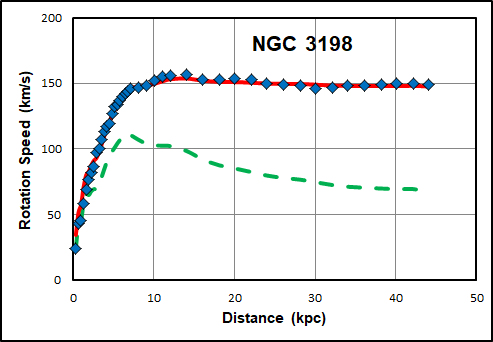
\includegraphics[width=0.8\textwidth]{chapters/c2/figure/ngc3198_sparc}
    \end{center}
    \caption{The figure opposite shows the rotation curve for spiral galaxy NGC 3198. The blue diamonds are the observations and reveal the almost flat-like nature of the curve in the outer regions of the galaxy. The dashed green line is the curve for Newtonian gravity. It shows that the rotational velocity should decrease with distance from the galaxy center. The solid red line through the data points is the curve obtained by assuming a simple Gaussian energy scale variation and a simple Gaussian density distribution for the galaxy. 
 }
    \label{fig:rotation}
  \end{figure}
 	
	
Cosmic Microwave Background(CMB)  in Big Bang cosmology, is electromagnetic radiation as a remnant from an early stage of the universe, also known as ``relic radiation’’. 
On the cosmological scale, not only CMB showed evidence of Dark Matter, it also quantifies the amount of Dark Matter in the Universe.
Experiments measure the fluctuations of the power spectra of the CMB where Lamda-CDM model are used to  fit the data, which gives the value of the density of baryonic matter, Dark Matter, and Dark Energy.
	

\subsection{Brief history of dark matter theory}
The hot dark matter (HDM) theory\cite{Zeldovich:1982zz} was established in 1980 by Zel’dovich’ team.
 The HDM assumes that the light neutrinos made up the majority of the dark matter. 
It is natural to assume that the dark matter is the weakly coupled particle that already existed in the standard model. 
However, the conventional neutrino-dominated picture is ruled out by the early universe simulation study in 1983. \cite{White:1984yj} 
Afterward, scientists realize that only with the slow-paced particle, the so-called ``cold'' dark matter, can prevent the diffusion of small scale fluctuation. 
As a result, the early universe structure can be formed on all scales, which is consistent with the observation result. 
Therefore, the cold dark matter theory(CDM theory)\cite{PhysRevLett.48.223} was established in 1983 to explain the cosmic microwave background observation result.
 Nowadays, as an important part of the standard cosmological model,(LambdaCDM theory), the concept of cold dark matter is widely accepted across the astronomers. 

\section{ Weakly Interacting Massive Particles}
Although the existence of cold dark matter around galaxies and clusters is supported by cosmological observation,
 scientists still have no clue about what exactly the cold dark matter is. Based on the reductionism, the observation of 
cold dark matter indicates the existence of weakly interacting fundamental particles. 
And since the density fluctuation is derived by the cold dark matter candidate mass, and the small scale fluctuation is not supposed to be dissolved, 
the mass of cold dark matter candidate can not be light. 
Therefore, the WIMPs - weakly interacting massive particles becomes one of the best candidate particles that characterize the feature of cold dark matter. 
					

WIMPs have masses at the electroweak scale from a few GeV to $\mathcal{O}$(TeV), which matchs bserved relic density from CMB analysis.  Both in the two popular beyond SM models Supersymmetry (SUSY) and Extra-dimensions, there are WIMP candidates of DM particles.							
The electrically neutral lightest supersymmetric particle (LSP) predicted in an R-parity conserved scenario of minimal supersymmetric extension of the Standard Model (MSSM) is an ideal candidates of Dark Matter.  Among all possible choices, the most promising one is the lightest neutralino,which is the lightest state of mixtures of neutral electroweak gauginos and the neutral higgsinos. \cite{Feng:2010gw}	 						
Similar to the phenomenology of the MSSM, in minimal universal extra dimensions(MUED) model, each SM particle is accompanied by a partner particle at the first Kaluza-Klein (KK)  mode level.

Also, the MUED model possesses a geometric parity (KK
parity). The lightest partner state (which in MUED is the partner of the $U(1)_Y$ gauge boson) represents
Dark Matter candidate which matches the observed dark matter relic density.\cite{SERVANT2003391}

\section{ Search dark matter in collider experiment}
Dark Matter was observed through its gravitational interaction in galaxies. To explore  its further particle properties,
 several complementary detection methods are used as showed in ~\ref{fig:detection}\cite{Undagoitia_2015}: \textbf{direct detection} which aim to observe low-energy recoils (typically a few keVs) 
of nuclei induced by interactions with particles of dark matter, which (in theory) are passing through the Earth,
 \textbf{indirect detection} which search for products of the self-annihilation or decay of dark matter particles in outer space,
 and collider searches looking for WIMPs in Large Hadron Collider (LHC) proton beams. WIMPs particle be detected indirectly as 
(large amounts of) missing energy and momentum that escape the detectors, provided other (non-negligible) collision products are detected as 
it should have negligible interactions with normal visible matter. In the following chapters, we will focus on the last method.			

\begin{figure}[htbp]
  \begin{center}
    \includegraphics[width=0.5\textwidth]{chapters/c2/figure/DM_detection}
  \end{center}
  \caption{ Three types of DM particle($\chi$) detection via an interaction with SM particles(P): from right to left the annihilation of DM particles into SM particles (indirect detection), from bottom to top the scattering of DM particles off a nuclei (direct detection), and from left to right the production of DM particles at high energy colliders like the LHC.}
  \label{fig:detection}
\end{figure}



\section{Simplified model}
Sample text sample text sample text. Sample text sample text sample text.
Sample text sample text sample text. Sample text sample text sample text.
Sample text sample text sample text. \cite{SimplifiedModels-Alves2012}



\part{The LHC and ATLAS experiment}
\label{sec:experiment-part}
\chapter{The LHC}
\label{ch:lhc}
%P1, what is the LHC?
\par The Large Hadron Collider, abbreviated as LHC, is the most powerful proton-proton collider, located at CERN, Geneva, Switzerland. The LHC is installed in a 26.7 km tunnel that was built for last generation lepton collider between 1984 and 1989. The LHC tunnel, which is located from 45m to 170m below the surface, is composed of 8 straight sections and 8 arcs. Therefore, the LHC can be viewed as 8 octants. Each octant has an access point, which includes an elevator from surface to underground. Half of the LHC points are hosting the detector systems currently: ATLAS\cite{Aad:2008zzm} at Point 1, ALICE\cite{Aamodt:2008zz} at Point 2, CMS\cite{Chatrchyan:2008aa} at Point 5 and LHCb\cite{Alves:2008zz} at Point 8. The other 4 points are designed for LHC operation purposes.

%P2, the LHC, history, and future
\par Rome wasn's built in one day, neither was the LHC. The LHC was built on the infrastructure of the previous generation of colliders located at CERN. The LHC is the current frontier of the evolution chain shown in Fig~\ref{fig:c3cernaccs}: from Proton Synchrotron (1954)\cite{Gilardoni:2011za}, Super Proton Synchrotron (1976)\cite{Doble:2017syb}, Large Electron-Positron Collider (1984)\cite{LepInjectorStudy:1983aa}\cite{LepInjectorStudy:1983ab}, to Large Hadron Collider (2008)\cite{Bruning:2004ej}\cite{Buning:2004wk}. Both infrastructure and technology are utilized in an economic manner to support the most powerful collider in the world, the LHC. The proton beam can be accelerated at 7~\TeV~by the current LHC setup. Although the LHC has reached the frontier of the high energy of human experiment, it is not the end of the CERN collider evolution chain. Both the LHC upgrade plan\cite{ApollinariG.:2017ojx} and next generation collider design\cite{Benedikt:2018csr} have been proposed to sustain the prosperity of the CERN collider family.

\begin{figure}[htbp]
    \centering
    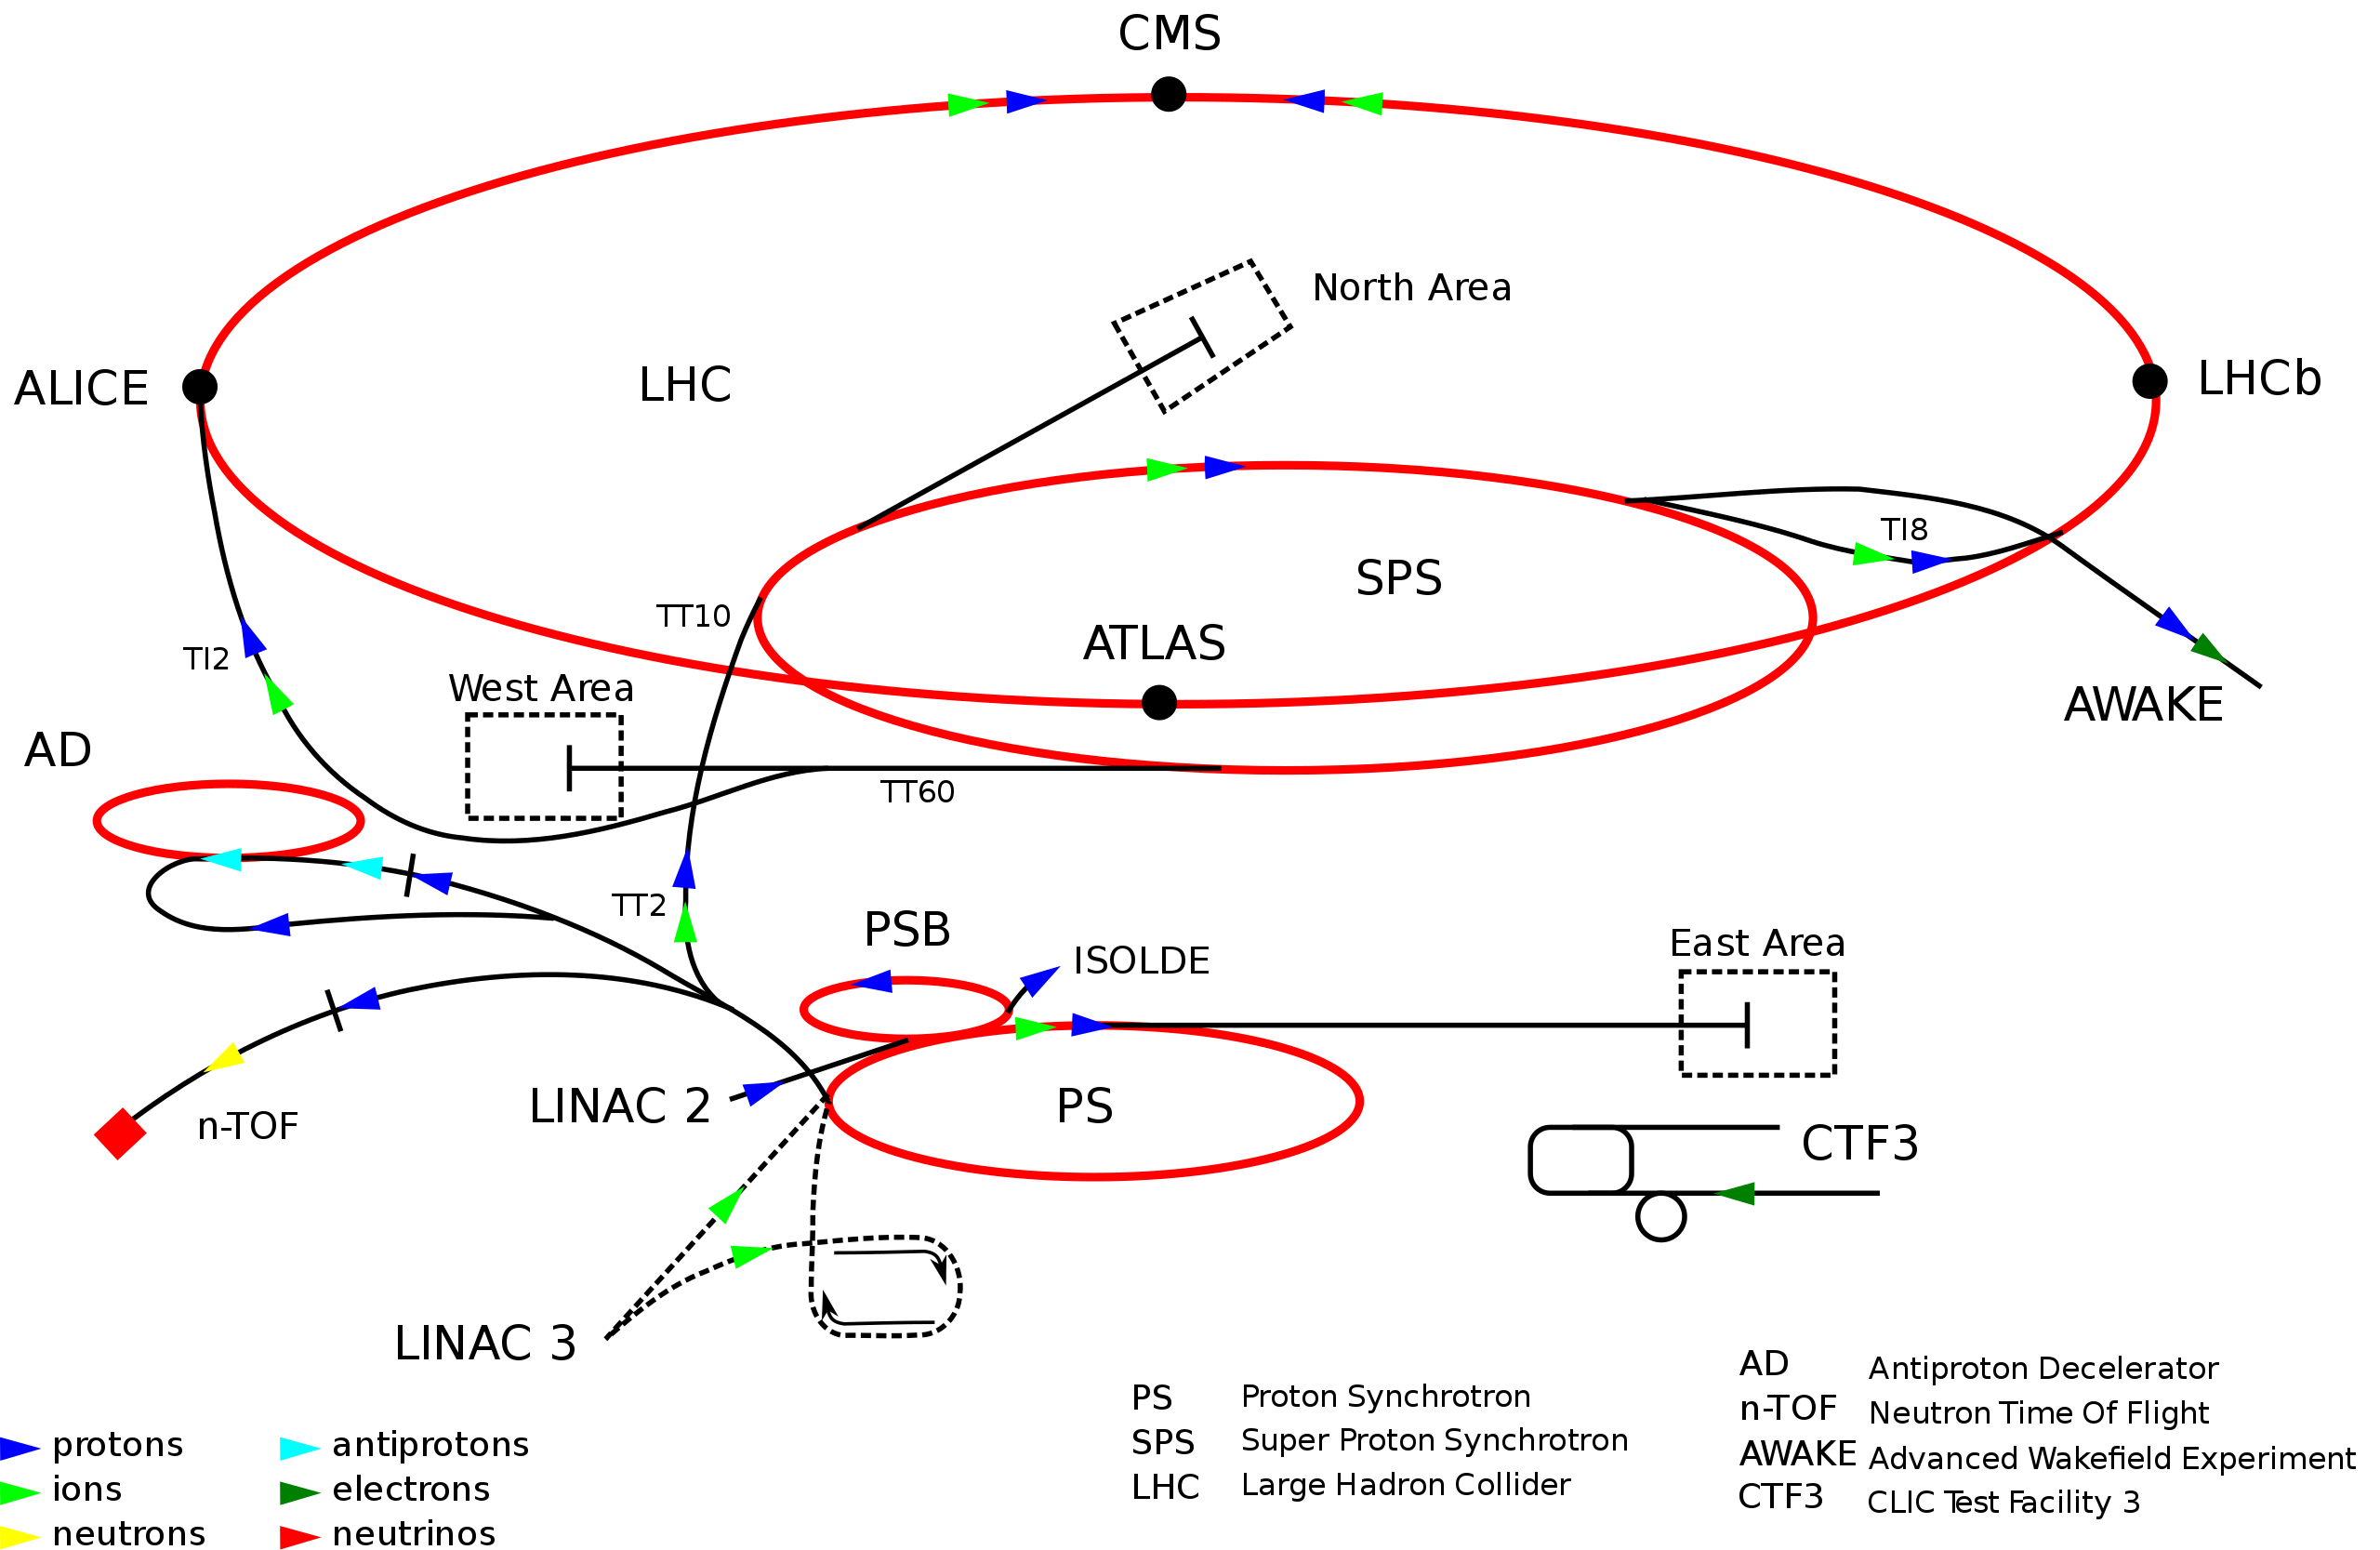
\includegraphics[width=0.8\textwidth]{chapters/c3/figures/cern-accelerator-complex.png}
    \caption{The LHC full injection chain.}
    \label{fig:c3cernaccs}
\end{figure}

\section{The LHC performance}
\label{sec:lhcs1}
%P1, the LHC performance and collision data collection: how many data do we take at what energy?
\par The aim of the LHC is to provide a stable, large amount of proton-proton collision events at the high energy frontier. Therefore, the LHC performance can be viewed as two parameters: the center-of-mass energy and integrated luminosity.

\subsection{Beam energy}
%P1, what energy? how to achieve
\par The center-of-mass energy is defined as the proton pair kinetic energy in the center-of-mass frame. Currently, the LHC is running at 13~\TeV~center-of-mass energy, with 6.5~\TeV~for each beam. Protons are accelerated and bended by electric field strips and 1232 superconducting dipole magnets around the LHC ring. Higher beam energy requires a stronger magnetic field, which requires to a higher electric current flowing in the magnets' superconducting coils.

\subsection{Luminosity}
%P1, how many data, lumi, definition, equation
\par The integrated luminosity, defined as the number of collision events produced by the LHC inside the particle detector, reflects the number of collisions delivered by the LHC. The integrated luminosity is determined by the LHC instantaneous luminosity, the beam cross-section and total LHC collision time.

\par The LHC luminosity can be calculated by Eq~\ref{eq:c3lumi}, where $N_{b}$ is the number of protons per bunch, $n_{b}$ is number of filled bunches per beam, $f_{r}$ is the frequency of the beam circling the ring, $\gamma_{r}$ is the relativistic gamma factor of the protons, $\epsilon_{n}$ is the normalized transverse beam emittance, $\beta^{*}$ is the measure of beam width in the longitudinal direction, $F$ is a geometric factor which accounts for the non-zero crossing angle between two beams:

\begin{equation}
  L = \frac{N_{b}^{2}n_{b}f_{r}\gamma_{r}4\pi\epsilon_{n}\beta^{*}}{F},
  \label{eq:c3lumi}
\end{equation}

\par The LHC can be running on different luminosity modes, while the detector system needs to be tuned to adapt the various LHC luminosity. The last parameter, total LHC collision time, is an operational parameter that depends on the collider and detector operation teams. The LHC delivered around 156~\ifb~data during the Run 2 period as shown in Fig~\ref{fig:lumi}.
\begin{figure}[htbp]
    \centering
    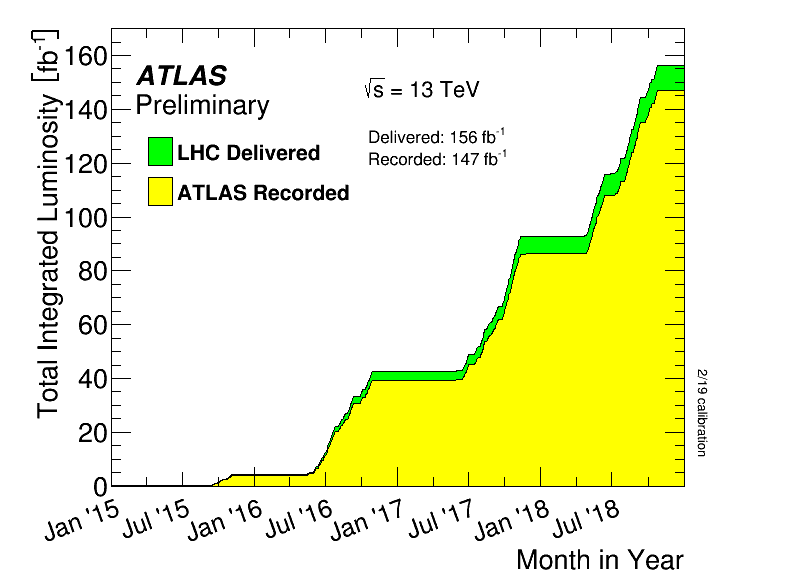
\includegraphics[width=0.8\textwidth]{chapters/c4/figures/intlumivstimeRun2}
    \caption{Cumulative luminosity versus time delivered to ATLAS (green), recorded by ATLAS (yellow) during stable beams for pp collisions at 13~\TeV~centre-of-mass energy in 2015-2018.}
    \label{fig:lumi}
\end{figure}

\section{The LHC operation}
\label{sec:lhcs1}
%P1, the LHC operation and detector operation, why beam mode
%\par The LHC is a collider with extremely complicated hardware and software design. Fortunately, the LHC team provide a concise operational guide to make physicists understand the LHC running status, which is very helpful during the detector operation. The LHC running status is very important for the detector operation, for example, the detector operator needs to monitor the LHC status and prepare detector configuration, like trigger menu, according to the beam injection notification. Normally, detector operators arrange the detector related activities according to the beam mode.

%P2, beam mode, table
\par The LHC beam modes are explained in Table~\ref{tab:c3lhcbeammode}. The beam modes describe the status of the beam related activities in the LHC. A successful beam injection starts with BEAM SETUP mode, which means beam circulating inside the Super Proton Synchrotron and waiting to be injected into the LHC. Then, a probe beam will be injected into the LHC ring as a trial, which is INJECTION PROBE BEAM mode. After that, INJECTION SETUP BEAM comes to measure the beam properties. After all the previous preparation, the physics injection finally comes into the LHC, which is called INJECTION PHYSICS BEAM. Normally, the detector operators need to get the detector system prepared when an injection physics beam happens. Then, the proton beam will be accelerated in the LHC with the PRERAMP and RAMP mode. The LHC system operators work on final machine adjustment at the FLAT TOP mode, and the beam impact parameter is reduced during the SQUEEZE mode. Finally, the beam is aligned in the ADJUST mode and STABLE BEAM mode will happen. Only the data taken during the STABLE BEAM mode will be used in physics analysis.

\begin{table}[htbp]
\fontsize{10 pt}{1.2 em}
\selectfont
\begin{centering}
\caption{\label{tab:c3lhcbeammode} LHC beam modes.}
\hspace*{-4ex}
\begin{tabular}{|c|c|c|}
\hline
 Mode Name &  Description \\
\hline
 SETUP & \specialcell{Beam in transfer line, but not in the ring} \\
\hline
 ABORT & \specialcell{Recovery mode following beam drop} \\
\hline
 INJECTION PROBE BEAM & \specialcell{Ring is injected with test beam for safe circulating} \\
\hline
 INJECTION SETUP BEAM & \specialcell{Beam measurement going on after probe beam\\ but before injection physics beam} \\
\hline
 INJECTION PHYSICS BEAM & \specialcell{Beam for physics is injected in the ring} \\
\hline
 PRERAMP & \specialcell{Injection done, prepare for ramp} \\
\hline
 RAMP & \specialcell{Ramp up the beam energy} \\
\hline
 FLAT TOP & \specialcell{Ramp done, pre-squeeze checks} \\
\hline
 SQUEEZE & \specialcell{Squeezing the beam size} \\
\hline
 ADJUST & \specialcell{Preparing for collision or after collision} \\
\hline
 STABLE BEAMS & \specialcell{Stable collision, detector should taking data} \\
\hline
 UNSTABLE BEAMS & \specialcell{Unstable beam because of sudden beam degradation} \\
\hline
 BEAM DUMP WARNING & \specialcell{Beam dump warning in case of emergency beam dump} \\
\hline
 BEAM DUMP & \specialcell{End of physics collision} \\
\hline
 RAMP DOWN & \specialcell{Ramp down beam energy after programmed dump} \\
\hline
 CYCLING & \specialcell{Pre-cycle before injection\\ following access, recovery, etc} \\
\hline
 NO BEAM  & \specialcell{No beams exist} \\
\hline
\end{tabular}
\par\end{centering}
\end{table}

\chapter{The ATLAS experiment}

Sample text sample text sample text. Sample text sample text sample text.
Sample text sample text sample text. Sample text sample text sample text.
Sample text sample text sample text. Sample text sample text sample text.
Sample text sample text sample text. Sample text sample text sample text.
Sample text sample text sample text. \cite{Grosz_and_Sidner_1986}

\section{ATLAS detector system}
Sample text sample text sample text. Sample text sample text sample text.
Sample text sample text sample text. Sample text sample text sample text.
Sample text sample text sample text. Sample text sample text sample text.

\subsection{Inner detector}
Sample text sample text sample text. Sample text sample text sample text.
Sample text sample text sample text. Sample text sample text sample text.
Sample text sample text sample text. Sample text sample text sample text.

\subsubsection{Pixel detector}
Sample text sample text sample text. Sample text sample text sample text.
Sample text sample text sample text. Sample text sample text sample text.
Sample text sample text sample text. Sample text sample text sample text.

\subsubsection{Semiconductor Tracker}
Sample text sample text sample text. Sample text sample text sample text.
Sample text sample text sample text. Sample text sample text sample text.
Sample text sample text sample text. Sample text sample text sample text.

\subsubsection{Transition Radiation Tracker}
Sample text sample text sample text. Sample text sample text sample text.
Sample text sample text sample text. Sample text sample text sample text.
Sample text sample text sample text. Sample text sample text sample text.

\subsection{Calorimeter}
Sample text sample text sample text. Sample text sample text sample text.
Sample text sample text sample text. Sample text sample text sample text.
Sample text sample text sample text. Sample text sample text sample text.

\subsubsection{Liquid Argon Calorimeter}
Sample text sample text sample text. Sample text sample text sample text.
Sample text sample text sample text. Sample text sample text sample text.
Sample text sample text sample text. Sample text sample text sample text.

\subsubsection{Tile Calorimeter}
Sample text sample text sample text. Sample text sample text sample text.
Sample text sample text sample text. Sample text sample text sample text.
Sample text sample text sample text. Sample text sample text sample text.

\subsection{Muon Spectrometer}
Sample text sample text sample text. Sample text sample text sample text.
Sample text sample text sample text. Sample text sample text sample text.
Sample text sample text sample text. Sample text sample text sample text.

\subsubsection{Thin Gap Chambers}
Sample text sample text sample text. Sample text sample text sample text.
Sample text sample text sample text. Sample text sample text sample text.
Sample text sample text sample text. Sample text sample text sample text.

\subsubsection{Resistive Plate Chambers}
Sample text sample text sample text. Sample text sample text sample text.
Sample text sample text sample text. Sample text sample text sample text.
Sample text sample text sample text. Sample text sample text sample text.

\subsubsection{Monitored Drift Tubes}
Sample text sample text sample text. Sample text sample text sample text.
Sample text sample text sample text. Sample text sample text sample text.
Sample text sample text sample text. Sample text sample text sample text.

\subsubsection{Cathode Strip Chambers}
Sample text sample text sample text. Sample text sample text sample text.
Sample text sample text sample text. Sample text sample text sample text.
Sample text sample text sample text. Sample text sample text sample text.

\section{Event reconstruction}
Sample text sample text sample text. Sample text sample text sample text.
Sample text sample text sample text. Sample text sample text sample text.
Sample text sample text sample text. Sample text sample text sample text.

\subsection{Tracks}
Sample text sample text sample text. Sample text sample text sample text.
Sample text sample text sample text. Sample text sample text sample text.
Sample text sample text sample text. Sample text sample text sample text.

\subsection{Electrons}
Sample text sample text sample text. Sample text sample text sample text.
Sample text sample text sample text. Sample text sample text sample text.
Sample text sample text sample text. Sample text sample text sample text.

\subsection{Jets}
Sample text sample text sample text. Sample text sample text sample text.
Sample text sample text sample text. Sample text sample text sample text.
Sample text sample text sample text. Sample text sample text sample text.

\subsection{Missing transverse momentum}
Sample text sample text sample text. Sample text sample text sample text.
Sample text sample text sample text. Sample text sample text sample text.
Sample text sample text sample text. Sample text sample text sample text.

\subsection{Muons}
Sample text sample text sample text. Sample text sample text sample text.
Sample text sample text sample text. Sample text sample text sample text.
Sample text sample text sample text. Sample text sample text sample text.

\section{Event simulation}
Sample text sample text sample text. Sample text sample text sample text.
Sample text sample text sample text. Sample text sample text sample text.
Sample text sample text sample text. Sample text sample text sample text.

\subsection{Event generator}
Sample text sample text sample text. Sample text sample text sample text.
Sample text sample text sample text. Sample text sample text sample text.
Sample text sample text sample text. Sample text sample text sample text.

\subsection{Detector simulation}
Sample text sample text sample text. Sample text sample text sample text.
Sample text sample text sample text. Sample text sample text sample text.
Sample text sample text sample text. Sample text sample text sample text.



\part{Dark Matter search in the Higgs Boson associated $b\bar{b}$ decay}
\label{sec:analysis-part}
%TODO, how many chapters do we need for this analysis section?
%introduction, object tagging? signal selection, background estimation, statistical interpretation
<<<<<<< HEAD
\chapter{Boosted Xbb tagging}

Sample text sample text sample text. Sample text sample text sample text.
Sample text sample text sample text. Sample text sample text sample text.
Sample text sample text sample text. Sample text sample text sample text.
Sample text sample text sample text. Sample text sample text sample text.
Sample text sample text sample text.

\section{Sample section}
Sample text sample text sample text. Sample text sample text sample text.
Sample text sample text sample text. Sample text sample text sample text.
Sample text sample text sample text. Sample text sample text sample text.

\subsection{Sample subsection}
Sample text sample text sample text. Sample text sample text sample text.
Sample text sample text sample text. Sample text sample text sample text.
Sample text sample text sample text. Sample text sample text sample text.

\subsection{Sample subsubsection}
Sample text sample text sample text. Sample text sample text sample text.
Sample text sample text sample text. Sample text sample text sample text.
Sample text sample text sample text. Sample text sample text sample text.

\section{Sample section}
Sample text sample text sample text. Sample text sample text sample text.
Sample text sample text sample text. Sample text sample text sample text.
Sample text sample text sample text. Sample text sample text sample text.

\subsection{Sample subsection}
Sample text sample text sample text. Sample text sample text sample text.
Sample text sample text sample text. Sample text sample text sample text.
Sample text sample text sample text. Sample text sample text sample text.

=======
\chapter{Physcis Objects}

\label{ch:objects}
This chapter introduced the physics objects used in this thesis in the reconstruction of events. 
 The reconstruction of primary vertices is described in Section~\ref{sec:pv}. 
The reconstruction of electrons, muons and taus are described in Section~\ref{sec:el}, Section~\ref{sec:mu} and Section~\ref{sec:taus}.
%Taus, which are also reconstructed as jets, are described in Section~\ref{sec:tau}. 
Different types of jets that are used by this analysis in different kinematic regions are described in Section~\ref{sec:jets}. 
The reconstruction of missing transverse energy (\met) and missing transverse energy significance, is discussed in Section~\ref{sec:met}. 
Finally Higgs tagging is described in detail in Section~\ref{sec:higgs}. 


\section{Inner Detector Tracks and Primary Vertex}
\label{sec:pv}
\par The tracks in the inner detector are based on fitting a trajectory model to a set of measurements using a sequence of algorithms
~\cite{Cornelissen:1020106}.
\par The inside-out algorithm, which is the baseline algorithm and is designed for efficient reconstruction of primary particles. 
It starts with three-point seeds in the silicon detectors and adds hits moving away from the interaction point using a combinatorial Kalman filter 
and tracks are extended into the TRT.
\par Then reconstruction of secondary particles produced by the interactions of the primary particles is achieved by Back-tracking. 
Back-tracking means a track search starts from segments reconstructed in the TRT and extends inwards by adding silicon hits. 
TRT-standalone tracks refer to tracks from TRT segment without extension into the silicon detectors.					
\par The transverse and longitudinal impact parameters of a track are referred to as $d_0$ and $z_0$ and their resolutions as $\sigma_{d_0}$ 
and $\sigma_{z_0}$. 
\par Each beam generates multiple track vertices, and the vertices are reconstructed from the available inner detector tracks.
\par All vertices with at least two associated tracks are retained as valid primary ver- tex candidates. 
The output of the vertex reconstruction algorithm is a set of three dimensional vertex positions and their covariance matrices. 
The primary vertex is selected as the one with the largest $\sum p_T^2$, where the sum is over all associated tracks. 
The basic track selection criteria are summarized in Table~\ref{tab:pv}.

\begin{table}[tbh]
\centering
\scriptsize
\begin{tabular}{|l|c|c}

\hline
 Aim& Selection \\
\hline
Reject soft fake tracks &$p_T> 0.4~GeV$ \\
\hline
In ID fiducial volume &$|\eta| < 2.5$ \\
\hline 
    Enough hits for track reconstruction & More than 9 hits between the Pixel\&SCT detectors for $|\eta|\le 1.65$\\
\hline 
    Enough hits for track reconstruction & More than 11 hits between the Pixel\&SCT detectors for $|\eta|\ge 1.65$\\
    
\hline 
 Good hit quality& Less than 2 hits in a SCT detector layer shared by multiple tracks\\
\hline 
 Good hit quality& Less than 1 hits in a Pixel detector layer shared by multiple tracks\\
\hline
 Good hit quality&0 missing hit in the Pixel detector when a hit is expected\\
\hline 
Good hit quality&Less than 1 missing hits in the SCT detector when hits are expected\\
 \hline
\end{tabular}
\caption{Selection criteria for track to reconstruct primary and pile-up vertices.}
\label{tab:pv}

\end{table}


\section{Electrons}
\label{sec:el}
\par Electron candidates are clusters of energy associated with ID tracks, 
where the final track-cluster matching is performed after the tracks have been fitted with a Gaussian-sum filter.
\par A few variables are checked to identify electron while suppressing background objects 
such as hadronic jets or converted photons~\cite{ATL-PHYS-PUB-2015-041}. 
They are the hits in the silicon detectors, including a hit on the IBL, and a likelihood discriminator, 
which combines the shower shape information provided by the highly segmented calorimeter, hits in the high-threshold TRT, 
compatibility of the tracking and calorimeter information, track quality information, 
as well as the impact parameter in the transverse plane ($|d_0|$) and its significance ($\frac{|d_0|}{\sigma_{d_0}}$).
\par Electron isolation measures the detector activity around an electron candidate, 
and can be used to further reject backgrounds such as electrons originating from converted photons produced in hadron decays, 
electrons from heavy flavor hadron decays, and light hadrons misidentified as electrons.
\par There are several working points of the likelihood variable which depends on how strict the requirements we require on electrons. 
This analysis uses the LooseLLHBLayer working point. In addition, this analysis applies two categories of electrons on electrons:
VHLoose and ZHSignal. The definitions of VHLoose and ZHSignal electrons are summarized in Table~\ref{tab:el}.
\begin{table}[tbh]
\centering
\begin{tabular}{|l|c|c|c|c|c|c|c}
\hline
Electron Type & $|p_T|$ & $|\eta|$ & $\frac{|d_0|}{\sigma_{d_0}}$ & $z_0\dot sin\theta$ & Likelihood & Isolation \\
\hline 
VHLoose &$>7$&$<2.47$&$<5$&$<0.5$&LooseLLHBLayer&LooseTrackOnly\\
\hline 
ZHSignal&$>7$&$<2.47$&$<5$&$<0.5$&LooseLLHBLayer&LooseTrackOnly\\
\hline

\end{tabular}
\caption{Definitions for the different categories of electron.}
\label{tab:el}
\end{table}
\par The VHLoose definition is used in the Signal Region where ZHSignal definition is used in some Control Regions, since the VHLoose definition is looser.
 
\section{Muons}
\label{sec:mu}
\par Muon reconstruction is performed based on information from the inner detector (ID), Muon S and calorimeters. As instructed in~\cite{Aad:2016jkr}, 
there are five types depending on different reconstruction methods.

\begin{itemize}
\item Combined muons are reconstructed by combining the hits of the ID track and MS track and the energy loss in the calorimeter;
\item Segment-tagged muons are formed from a track in the ID if it is associated with at least one track segment in the MDT or CSC chambers. 
 It capture muons passing only one layer of MS chambers, due to their low \pt~or reduced MS acceptance in the region.
\item Extrapolated muons are reconstructed based only on the MS track and a loose requirement on compatibility with originating from the IP. 
 They are used to extend the acceptance for muon reconstruction into the region $2.5 <\eta< 2.7$. 
 The muon is required to traverse at least two layers of MS chambers to provide a track measurement, but three layers are required in the forward region.

\item Calorimeter-tagged muons. In the region of $|\eta< 0.1$, ID tracks with $15 ~GeV < p_T < 100 ~GeV$ are identified as muons if their energy deposits in the calorimeter 
 match with minimum ionizing particles. They recover muon acceptance in the region where the MS is only partially instrumented.

\end{itemize}
\par Similar to Electron reconstruction, there are different muon identification working point. This analysis chose ``Loose'', defined as muons reconstructed using any reconstruction methods, 
and ``Medium'', reconstructed using either the Combined muon or Extrapolated muon methods.
\par The VHLoose definition is used in the Signal Region where ZHSignal definition is used in some Control Regions, since the VHLoose definition is looser.					
\par As showed in Table~\ref{tab:mu}, this analysis applied additional criteria to muons in different regions. 
A tighter selection is required in Control Regions for a high muon purity and a looser selection when muons are not desired and are vetoed in the Signal Region.
\begin{table}[tbh]
\centering
\begin{tabular}{|l|c|c|c|c|c|c|c}

\hline
  Electron Type & $|p_T|$ &$|\eta|$ & $\frac{|d_0|}{\sigma_{d_0}}$&$z_0 sin\theta$ & Likelihood &Isolation \\
\hline 
VHLoose &$>7$&$<2.7$&$<3$&$<0.5$&Loose&LooseTrackOnly\\
\hline 
WHSignal &$>25$&$<2.5$&$<3$&$<0.5$&Medium&FixedTrackTTTight\\
\hline 
ZHSignal &$>25$&$<2.5$&$<3$&$<0.5$&Loose&LooseTrackOnly\\
\hline
\end{tabular}
\caption{Definitions for the different categories of muons.}
 \label{tab:mu}
\end{table}


\section{Taus}
\label{sec:taus}
% Tau, what and why
\par Tau lepton veto algorithm is needed in the analysis since it is not interested in the signal events. Tau particle, unlike its lighter lepton buddy, electron and muon, 
is the only lepton that can decay into hadrons. The branching ratio of hadronically tau decay is approximately 64.79\%. Therefore, it is important to reject hadronically decayed 
tau events in the hadronic analysis.

% How to reject tau with Loose Tau ID
\par Hadronicallly decayed tau can be reconstructed as small-radius jets and identified with a tree-based machine learning algorithm. A typically hadronically decayed tau jet 
can be characterized with either one or three charged hadrons, which can be applied to the tree-based classifiers to differentiate from QCD jets. With the trade-off of selection 
efficiencies and fake rate, three classifiers, loose, medium, tight, can be determined. More details can be found in \cite{ATL-PHYS-PUB-2015-045}. 
In order to reduce the hadronically decayed tau to a maximum extent, the loose working point is chosen to build the tau veto condition, together with the baseline section of $p_T > 25 GeV$ and $|\eta| < 2.5$.

\section{Jets}
\label{sec:jets}
\par In pp collisions, almost immediately after being produced, a quark or gluon fragments and hadronises, leading to a collimated spray of energetic hadrons -- 
a jet~\cite{Salam:2009jx}. There exist many different jet clustering algorithms to measure the jet properties. 
\par Among all jet finding algorithms, the anti-$k_T$ algorithm~\cite{Cacciari:2008gp} is most commonly used. This algorithm flavors clusterings that involve hard particles, 
and the jets then grow outwards around hard ``seeds''. R is in the denominator of the clustering distance metric. It determines the radial size of the jet in $\eta-\phi$ plane.
\par Calorimeter jets are reconstructed by combining topological clusters of energy deposits in the calorimeter~\cite{Aad:2011he}, while the inputs to track jet clustering are inner detector (ID) tracks. 
The small R = 0.4 calorimeter jets are used for b-quark reconstruction in the resolved topology. For jets that are from collimated decay products of heavy particles or low \pt~gluons, 
a large cone size are used to contain all of the decay products. Large-R jets are defined in ATLAS collaboration as jets reconstructed with the anti-$k_T$ algorithm with R = 1.0 using calibrated 
calorimeter clusters.The large R calorimeter jets are used for Higgs boson reconstruction in the boosted topology in this analysis.
\par In this iteration of the analysis, the variable radius track jet replaced the small fixed R = 0.2 track jets to be used for b-quark identification inside the large-R jets.

\subsection{Calorimeter jets}
\label{sec:calo}
 \par Topological clusters (topo-cluster) are cells are clustered together to reconstruct such particle shower, due to fine granularity in calorimeters. 
 The topo-cluster reconstruction is based on cell signal significance S/N, defined as the ratio of cell energy at electromagnetic energy scale over average expected noise. 
 The reconstruction starts from a seed cell with signal significance above the threshold of S/N = 4. Then the neighbouring cells with signal significance over S/N = 2 are included iteratively.
 Finally, all calorimeter cells neighbouring the formed topo-cluster are added. After the iteration, one outer layer of all surrounding cells are added, 
 so the resulting topological cluster is at the electromagnetic scale.
\par For large R jets, a local hadronic calibration (LCW) is then applied at cluster-by-cluster level to correct for non-compensation effect which underestimating the energy of hadronic particles.
For small R jets, EM scale becomes the default for ATLAS in Run 2.
\begin{figure}[htbp]
 \begin{center}
 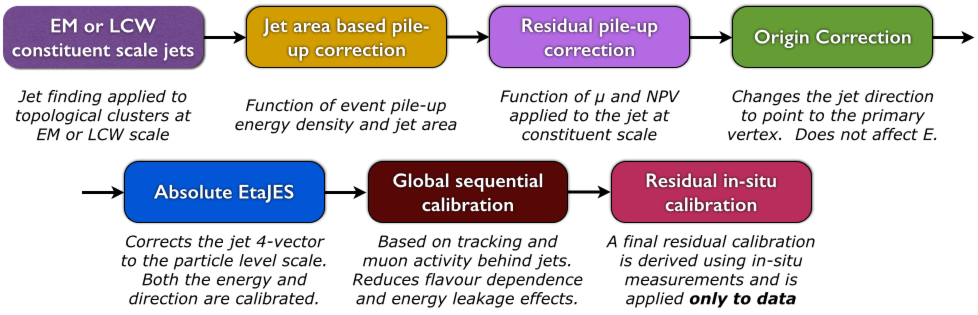
\includegraphics[width=1\textwidth]{chapters/c5/figures/jet_calib}
 \end{center}
 \caption{Calibration stages for reconstructed jets.}
 \label{fig:jet-calib}
\end{figure}
\par After jets are reconstructed, calibration needs to be applied on the four momentum of reconstructed jet to restore it back to particle-level energy scale.
A series of calibrations are applied after jet clustering as shown in Fig~\ref{fig:jet-calib}.

\begin{itemize}
\item \textbf{Origin correction} The kinematic observables of each topo-cluster are recalculated using the vector from the primary hard-scattering vertex to the topo-cluster centroid as its direction. The resolution of $\eta$ can be improved in this step. The jet energy is unaffected.
\item \textbf{Jet area-based pile-up correction} This step are designed to remove the excess energy from pile-ups. The area-based \pt~density subtraction is applied event-by-event~\cite{Cacciari:2007fd}. The \pt~density is estimated using the medium of \pt~density of all jets in the event calculated by \pt/A, where A is the jet area.
\item \textbf{Residual pile-up correction} A residual \pt~dependency on in-time pile-up $N_{PV}$ and out-of-time pile-up $\mu$ is roughly linear. So the linear correction is applied with coefficients derived from MC simulation. 
\item \textbf{Absolute MC-based calibration} An absolute jet energy and $\eta$ correction is derived from MC simulation. The average energy response is defined as the mean of $E_{reco}/E_{truth}$ binned in $E_{truth}$ and $\eta_{jet}$. Similar correction is done for $\eta$. 
\item \textbf{Global sequential calibration} The global sequential calibration (GSC) method~\cite{Aad:2011he} is applied to improve resolution of JES. In this step, JES depends on five features which accounts for different aspects and the calibration factor is derived from MC. The procedure is similar to the absolute JES.
\item \textbf{Residual in situ calibration} This steps aims at correcting difference between data and MC. For jets up to 950 GeV and with $|\eta| < 0.8$, Z+jest and $\eta$+jet balance is used, while, for high-\pt~jet up to 2 TeV, multijet balance is used.
\end{itemize}
\par The larger the jet size, the more chances there are particles from underlying events, 
pile-up interactions and soft component of the radiation to contaminate the jet. Thus for large R jets, three techniques of jet grooming are developed:
split-filtering~\cite{Butterworth:2008iy}, pruning~\cite{Ellis:2009me} and trimming~\cite{Krohn:2009th}. 

\begin{itemize}
\item \textbf{Split-filtering} Large-R jets are first built with C/A algorithm. This algorithm includes splitting and filtering. 
 Splitting is to find the hard two-prong splitting substructure from massive parent particle. C/A jets are de-clustered by splitting jet into two pieces. De-clustering continues with the highest mass piece 
 until the requirements on mass-drop $\mu_{12} < \mu_{max}$ and momentum balance $\sqrt{y_{12}} > \sqrt{y_{min}}$ are met. 
 The momentum balance $y_{12} = \frac{min(p_{T1},p_{T2})}{m_{12}}\Delta R_{12} $ and mass-drop is defined as $\mu_{12} = max(m_1,m_2) m_{12}$, where $m_{12}$ 
 is the invariant mass of two pieces. If the requirements are not satisfied, the jet is discarded. Filtering aims at removing soft radiations that is irrelevant to the hard splitting process. 
 In filtering stage, constituents of surviving jet are reclsutered with subjet size of $R_{sub} = min(0.3,\Delta R_{12})$, where $\Delta R_{12}$ is taken from splitting stage.
\item \textbf{Pruning} Pruning is similar to trimming as it removes constituents with relative small $p_T$, while it has an additional wide-angle radiation veto. Large-R jets are first built with C/A or anti-$k_t$
 algorithm. Constituents of ungroomed large-R jet are then re-clustered with C/A algorithm based on $R_{cut}$ and $Z_{cut}$. In each pairwise clustering step, secondary constituents with wide-angle 
 $\Delta R_{12} > R_{cut} \times \frac{2M}{p_T}$ or soft property are discarded. Definition of being soft is that $f_2 < Z_{cut}$ where $f_2$ is the fraction of softer constituent \pt~with respect to the pair.
\item \textbf{Trimming} Large-R jets are first built with C/A or anti-$k_t$ algorithm. This requires reclustering all of the jet’s constituents using the $k_T$ algorithm, 
 which flavors clustering low \pt~constituents first. This creates a set of subjets with radius parameter $R_{sub}$. 
 Subjets with an energy below some threshold fraction of the energy of the large-R jet are removed from the large R jet. 
 The trimmed large-R jet will be used to reconstruct Higgs candidates in boosted region.
\end{itemize}
\par The resulting jet is trimmed large-R jets, and is used to reconstruct Higgs candidates when the b-quark decay products of the Higgs are too collimated to resolve by two small-R jets.

\par Small-R jets used in the analysis could be divided into two categories: central jets and forward Jets. Forward jets are small-R jets with $2.5 < |\eta| < 4.5$ and $p_T > 30 GeV$, and can be used by event selections to reduce backgrounds.
 Small-R jets with $|\eta| < 2.5$ and \pt~$> 20 GeV$ are called central jets and they are used to reconstruct Higgs candidates with low \pt~.
For central jets with $|\eta| < 2.4$ and $20 GeV < p_T < 60 GeV$, an additional requirement on jet vertex tagger value $JVT > 0.59$ are required. Details on the jet vertex tagger (JVT) is could be found here~\cite{Aad:2015ina}.



\subsection{Track jets}
\label{sec:track}


\par Track jets are jets built entirely from tracks reconstructed in inner detector via the same anti-$k_T$ algorithm as calorimeter jets. In Run 2, track jet b-tagging became the standard approach to resolve heavy flavor components from boosted decay of heavy resonances~\cite{ATL-PHYS-PUB-2015-035,ATLAS-CONF-2016-039}. Studies of track jet calibration can be found in~\cite{VanDenWollenberg:1981533}. 
\par In this thesis, two types of track jets are discussed. R = 0.2 track jets will be referred to as FR track jets, for fixed radius track jets, in contrast to the variable radius (VR) track jets which will be discussed later.

\par A track selection of input ID tracks is applied in order to suppress fake tracks and tracks from pile-up vertex. The selection criteria is summarized in Table~\ref{tab:trk}. With a relatively looser requirement on hits in the ID detectors compared to the track selection criteria for primary vertex reconstruction, it requires a small longitudinal impact parameter of the tracks with respect to the primary vertex to reject pile-up vertex.
\begin{table}	
\centering

    \scriptsize
\begin{tabular}{|l|c|c}
\hline
Aim & Selection \\					
\hline
Reject soft fake tracks &$p_T> 0.4 GeV$ \\
\hline
In ID fiducial volume &$|\eta| < 2.5$\\
\hline 
enough hits for track reconstruction & More than 7 hits between the Pixel and SCT detectors \\
\hline 
 good hit quality& Less than 1 hit in a Pixel shared by multiple tracks\\
\hline
 good hit quality&Less than 1 missing hit in the Pixel detector when a hit is expected\\
\hline 
good hit quality&Less than 2 missing hits in the SCT detector when hits are expected\\
 \hline
reject tracks from pile-up & $z_0 \dot sin(\theta) < 3 mm$\\
 \hline
\end{tabular}
\caption{Selection criteria for tracks to cluster track jets. }
\label{tab:trk}
\end{table}	
\par FR track jets are then built by applying anti-$k_T$ algorithm with R = {0.4, 0.3, 0.2} on selected tracks. Track jets in fiducial region with $p_T > 7 GeV$ and $|\eta| < 2.5$ are accepted as track jets with $p_T < 7 GeV$ are rejected as they are dominated by light jets~\cite{ATL-PHYS-PUB-2014-013}. 				
\par VR track jets are clustered using the anti-$k_t$ algorithm from tracks with the same selection criteria used for R = 0.2 track jets. The main feature of the VR track jet reconstruction~\cite{Krohn:2009zg}, compared to the FR jets is the \pt~dependence of the jet radius:
\begin{equation}
R \rightarrow R_{eff}(p_T) \approx \frac{\rho}{p_T}
\end{equation}
where the parameter $\rho$ shows how the effective jet radius scales with the \pt~of the pseudo-jet during the jet finding procedure, $R_{min}$ and $R_{max}$ are a lower and an upper cut on the jet radius.
To optimize the efficiency of double b-tagging over a wide mass, $ \rho = 30 GeV$, $R_{min} = 0.02$ and $R_{max} = 0.4$~\cite{ATL-PHYS-PUB-2017-010}.

\subsection{Ghost Association}
\label{sec:ga}

\par In practice, track jets are seldom used alone for object reconstruction and instead used along with the large calorimeter jets. Calorimeter jets are in charge of providing jet reconstruction while track jets are in charge of providing flavor tagging information. To match track jets to calorimeter jets is the first step for flavor tagging. 
\par Ghost association~\cite{Cacciari:2007fd,Cacciari:2008gn} is a method to associate the ``ghost'' (particles, jets or tracks) to jets by giving them negligible momentum and clustering them within the jets. This is to make sure that the hard-particle content of the jet is unaltered by the addition of the soft ghost particles during jet reclustering. The jet substructure after reclustering is unchanged compared to the previous jet, but with the addition of ``ghost'' as constituents.
\par An object (track, jet, truth particle) is ghost-associated to a jet if its ``ghost'' is clustered as a constituent of the jet.
\par Compared to $\Delta R$ association which matches objects based on angular distance, ghost association is more robust when dealing with overlapping jets or jets that are not cone-shaped.



\subsection{Flavor tagging}
\label{sec:track}
\par The identification of b jets is referred to as b-tagging or flavor tagging. After the fragmentation of b-quarks, about 70\% of the b-quark energy goes into the weakly decaying b-hadrons (~5 GeV). With an intrinsic life-time of $1.5 \times 10^{−12}$ s, the average decay lengths for b-hadrons of 30 GeV is about 3 mm, which could be measued with the high-precision tracking system in ATLAS.
The c-hadrons from b-hadrons decay also have similar average lifetimes, and thus leads to an additional decay. 
Several b-tagging algorithms are developed by studying the decay patterns. 				
\par ID tracks are used for these b-tagging algorithms, and tracks need to pass the basic quality cuts. 		
\par These three b-tagging algorithms below are used to provide complementary information and combined using boosted decision tree (BDT) to provide a score to distinguish between different flavors (c, b, light). 	
\begin{itemize}				
\item \textbf{Impact Parameter Based Algorithm (IP2D and IP3D)} 	
As shown in Fig.2 from the reference~\cite{ATL-PHYS-PUB-2015-022}, tracks from a displaced vertex have larger impact parameter than those coming from primary vertex. The probability density functions (PDFs) for the signed impact parameter significance of these tracks $\frac{d_0}{\sigma_{d_0}}$ and $\frac{z_0}{\sigma_{z_0}}$ are used to define ratios of the jet hypotheses of different flavors, and these are then combined in a single log likelihood ratio discriminant (LLR). While IP2D only uses transverse impact parameter, IP3D uses the 2D template with correlation between transverse and longitudinal direction.				
\par Both IP2D and IP3D assume that all tracks are independent and they are naive Bayesian models which ignore correlations between tracks. Besides, while it is easy to build 2D or 3D template histograms, it is technically hard to encode too many variables at the same time. To improve the results, new algorithm which makes use of the recurrent neural network with the same input tracks as IP2D/IP3D are developed in ATLAS b-tagging~\cite{ATL-PHYS-PUB-2017-003}. 
\item \textbf{Inclusive secondary vertex reconstruction algorithm (SV)} 	
The secondary vertex based algorithm explicitly reconstructs an inclusive displaced secondary vertex within the jet. Tracks passing quality cuts are first paired to form two-track vertex. And these two-track vertex would then be filtered to reject if coming from decay of long-lived particles such as $K_s$, $\Lambda$, photon conversion or hadronic interaction with detector materials. An inclusive secondary vertex would be fit using survived tracks using Kalman filter in an iterative way and certain quality cuts will be applied. 				
\item \textbf{Decay chain multi-vertex reconstruction algorithm (JetFitter)} 		 	 	 		The decay chain multi-vertex reconstruction algorithm is called JetFitter and studys the cascade decay structure of b-hadron and c-hadron coming out of it to reconstruct the hadron decay chain $Primary\ Vertex \rightarrow b \rightarrow c$ using a Kalman filter.		 	 	 		
\par Because unlike the SV algorithm, the vertex in JetFitter refers to the intersection between tracks and estimated decay chain direction and thus a vertex could have even only one track associated to it. Thus JetFitter typically has a much higher reconstruction efficiency, as well as a higher fake rate. To reduce the fake rate, a set of topological variables are built in JetFitter for discrimination purpose. 
\end{itemize}		

\par After running each b-tagging algorithms independently, output discriminative variables of each algorithm, as well as the kinematic properties of jets \pt~and $\eta$ are combined using BDT. The \pt~and $\eta$ joint distribution between signal and backgrounds re-weighted to match each other before training so that these kinematic variables are not treated as discriminative variables.
\par The training is performed on high purity ttbar and zprime MC samples with at least millions of events. While b-jets are used as signal jets, 
the background is a mixture of c-jets and light-jets. Three versions of mixture are available at ATLAS: MV2c00, MV2c10 and MV2c20. The number after character ``MV2c''
shows the percentage of c-jets in background mixture. 
Depending on the physics processes, users can choose the any of these three version.
The higher the number, the better the discrimination power against c-jets at the cost of less light-jet rejection. 
The performance of MV2c10 tagger~\cite{Varni:2655785} for discrimination against light-jet and c-jets can be found in Fig~\ref{fig:mv2c10}.

\begin{figure}[htbp]
 \begin{center}
 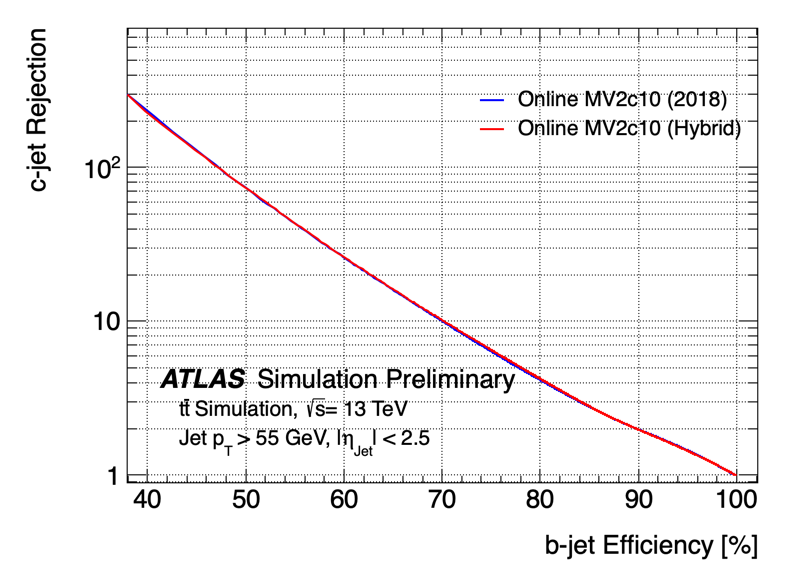
\includegraphics[width=0.4\textwidth]{chapters/c5/figures/ROC_cb}
 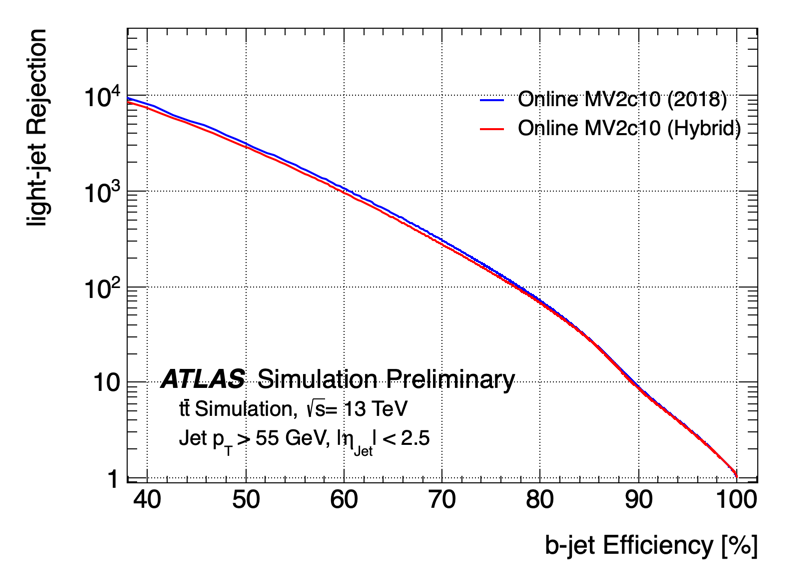
\includegraphics[width=0.4\textwidth]{chapters/c5/figures/ROC_lb}
 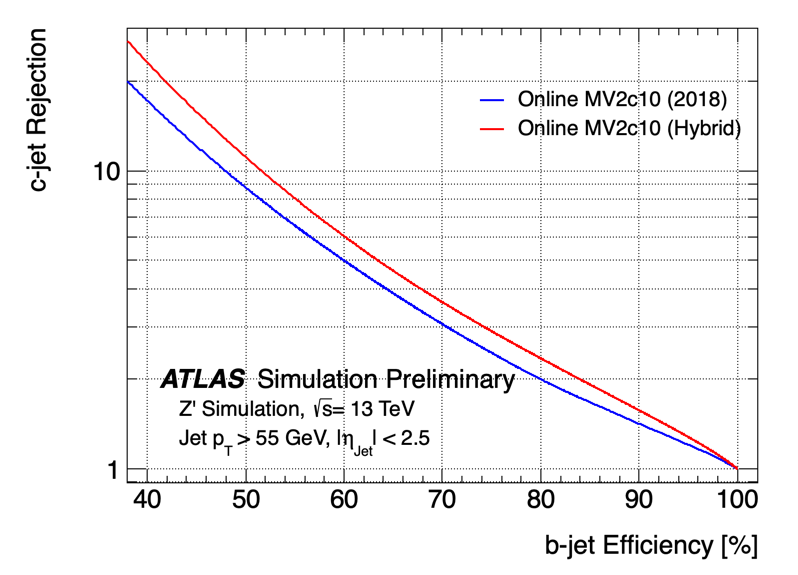
\includegraphics[width=0.4\textwidth]{chapters/c5/figures/ROC_cb_Zprime}
 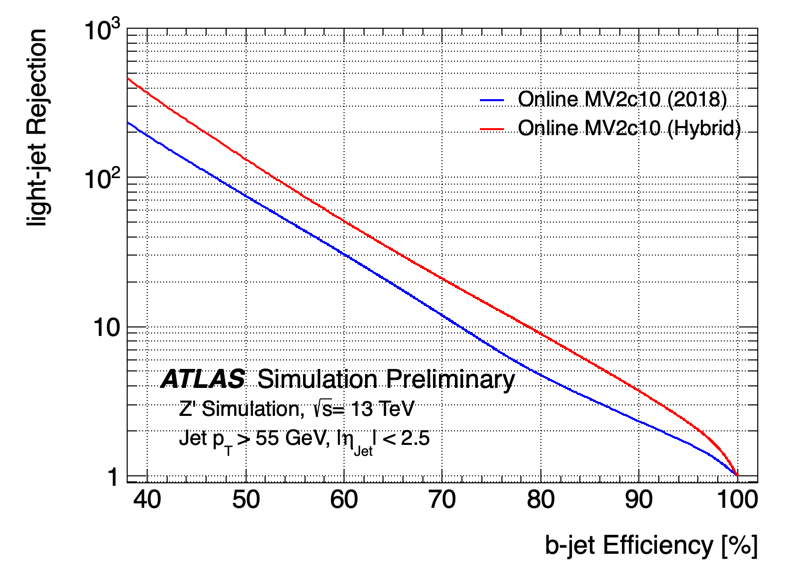
\includegraphics[width=0.4\textwidth]{chapters/c5/figures/ROC_lb_Zprime}
 \end{center}
 \caption{Expected performance of \textit{b}-tagging algorithm (MV2c10) for \textit{b}-jet triggers in 2018 data-taking (blue solid line) is compared to the same \textit{b}-tagging algorithm trained on the Hybrid training sample (red solid line).}
 \label{fig:mv2c10}
\end{figure}

\section{Messing Transverse Energy/Momentum (MET) and Missing Transverse Energy Sigificance}

\label{sec:met}
% What is MET
\par According to the conservation of momentum, the sum of the transverse memento of all particles produced in collisions is zero. Considering the existence of the non-detectable object, the transverse energies from detected objects are not balanced. The unbalanced part of transverse momentum is called ''missing transverse energy''(\met), or MET for short.

% How to calculate MET with/without Tracker fully involved.
\par As mentioned in the last paragraph, the \met~is derived by all other detectable objects. The \met~calculation is the most difficult object not only because it needs a full calculation of all detectable objects from various detectors, but also from the small fraction of energy deposits from unclustered parts of detectors. As a result, the \met~scale and \met~resolution are affected by many factors, such as missing Muons, mismeasured Jets, beam pile-up, etc. In the ATLAS experiment, the \met~reconstruction uses energy deposits in the calorimeters and muons tracks reconstructed in the muon detectors. Trackers' information is also used to recover the low Pt fraction that missed in the calorimeters \cite{ATLAS-CONF-2013-082}. Therefore, both hard objects (high \pt~), like electrons, jets, muons, etc, and soft objects, like track soft terms, are considered in the \met~reconstruction.

% MET significance
\par The uncertainty of \met~calculation result can be remarkably large due to the complexity of the reconstruction algorithm. Therefore, a significance variable can be introduced to describe the reliability of the derived \met. The \met~significance is defined as
$$ S=\frac{\met}{\sqrt{\sum_{i}E_{Ti}}}, $$
where the numerator is the amplitude of derived \met, and the denominator is the scalar sum of the detected objects that used when to reconstruct the \met. A high value of \met~significance suggests the event is more likely to container invisible object rather than resolution smearing.

\section{Higgs tagging}
\label{sec:higgs}
\par For Higgs particle with sufficiently low \pt, two outcoming b-quarks can be reconstructed individually as Small-R = 0.4 calorimeter jets. However, for Higgs particle with high \pt, 
the two outcoming b-quarks are too collimated be reconstructed using small-R jets.
``Higgs tagging'' in the thesis refers to the techniques used to identify boosted Higgs decays to b-quarks. The Higgs candidate is reconstructed as a trimmed large-R jet 
with two ghost-associated b-tagged subjets, reconstructing the b-hadrons.
\subsection{Higgs tagging with advanced subjets}

\par Three techniques, variable radius track jet Higgs tagging technique, Exclusive-kT (ExKt) and Center-of- Mass (CoM), for tagging a very boosted Higgs 
particle~\cite{ATL-PHYS-PUB-2017-010}, 
whose b-hadron decay products will become too collimated to resolve even with R = 0.2 track jets.
\par The definition of VR track jets could be found in Section~\ref{sec:jets}, as showed in~\ref{fig:vr}. And the parameters $\rho = 30 GeV$, $R_{min} = 0.02$ and $R_{max} = 0.4$ 
are chosen after scanning different $\rho$ and radius as showd in Fig.~\ref{fig:vr-scan}.


ExKt subjet refers to exclusive regions of interest using exclusive-kT declustering of large-R jet. 
And CoM jets are constructed via exclusive-kT declusting in center of mass frame instead of in the lab frame.
\begin{figure}[htbp]
 \begin{center}
  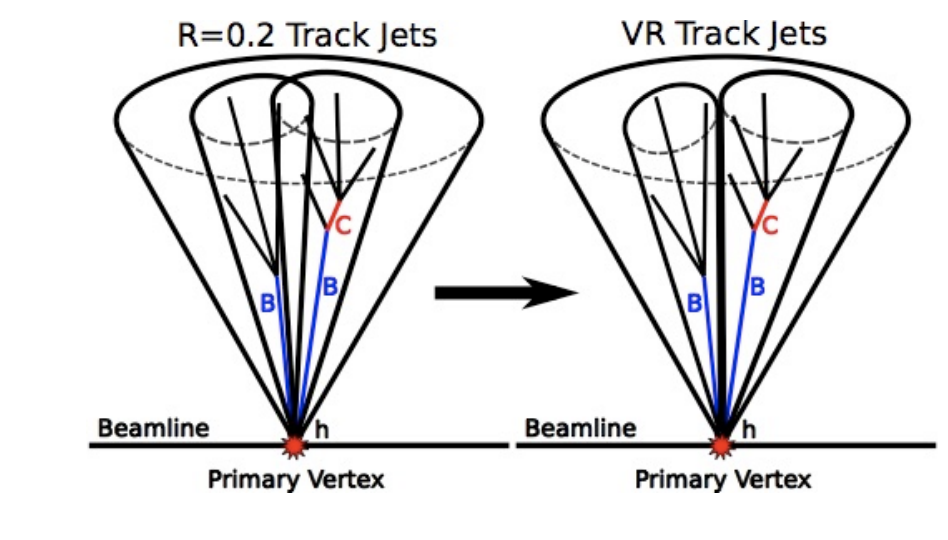
\includegraphics[width=0.6\textwidth]{chapters/c5/figures/VR}

 \end{center}
 \caption{A cartoon depicting how using VR track jets instead of R = 0.2 track jets.}
 \label{fig:vr}
\end{figure}
\begin{figure}[htbp]
 \begin{center}
  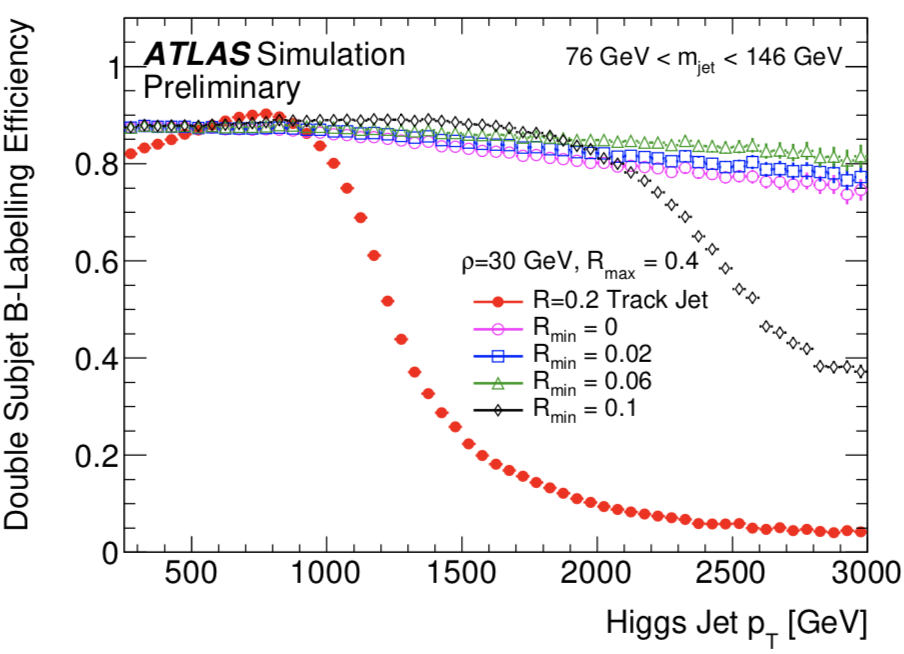
\includegraphics[width=0.4\textwidth]{chapters/c5/figures/r-vr}
  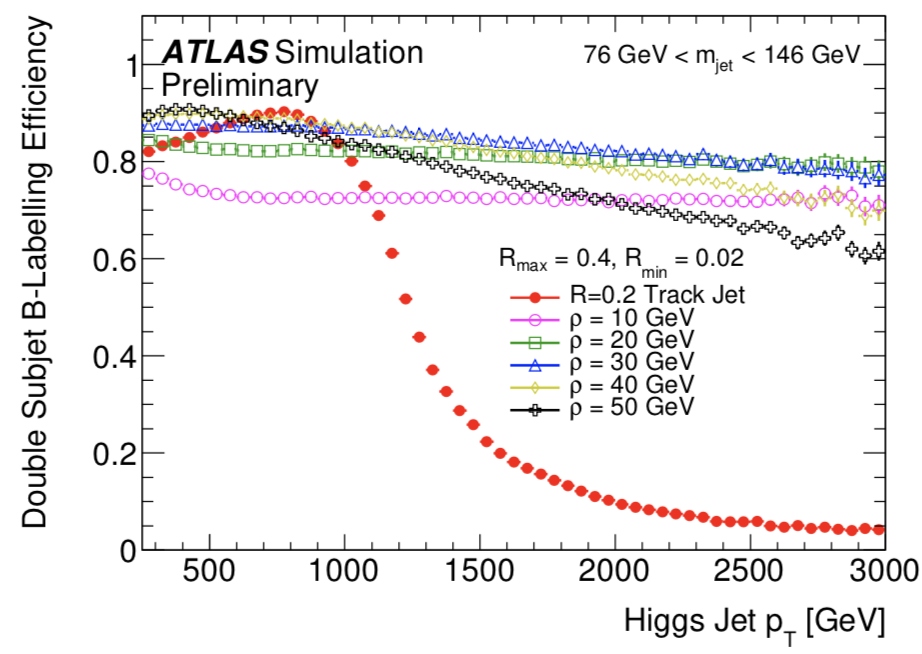
\includegraphics[width=0.4\textwidth]{chapters/c5/figures/rho-vr}

 \end{center}
    \caption{Higgs effiency using two VR track jets with different R parameter (Left) and $\rho$ parameter (Right)} 
 \label{fig:vr-scan}
\end{figure}
\par The double subjets b-labelling performance for the FR track jet, VR track jet, ExKt and CoM techniques could be found in Fig.~\ref{fig:higgs_pt}.
The plot shows a dramatic decrease for the R = 0.2 track jet technique as the Higgs jet \pt~becomes larger than 1.2 TeV where this is precisely the region where the 
R = 0.2 track jets are expected to merge. 
New techniques, however, could reconstruct Higgs jets with a \pt~of 3 TeV. And receiver operating characteristic (ROC) curves showing the Higgs jet tagging performance versus 
QCD jet rejection are shown 
in Fig.~\ref{fig:higgs_ROC}.


\begin{figure}[htbp]
 \begin{center}
  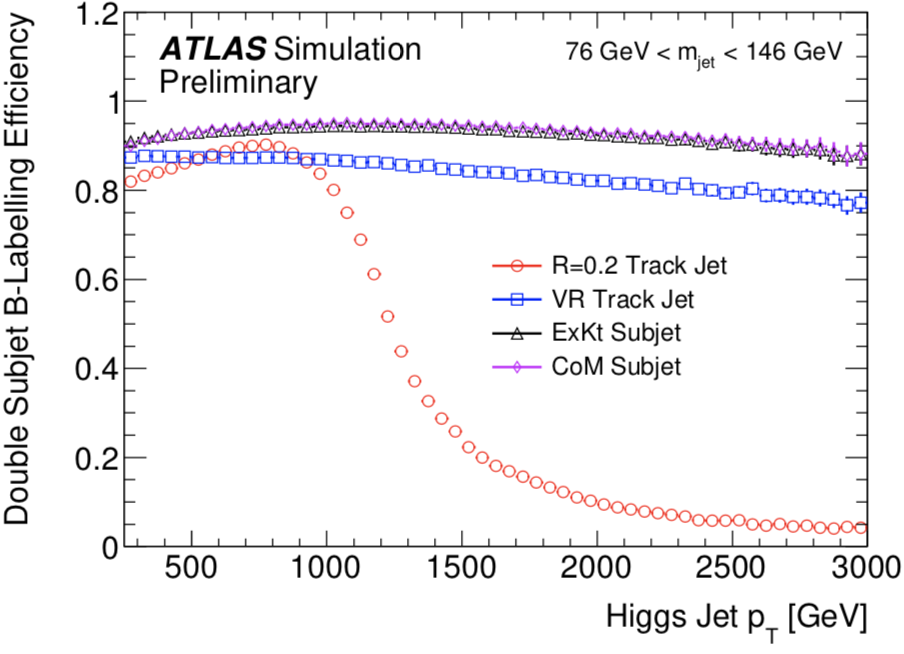
\includegraphics[width=0.6\textwidth]{chapters/c5/figures/higgs_pt}

 \end{center}
 \caption{Higgs efficiency using four different subjet techniques: R = 0.2 track jets, VR track jets, ExKt calorimeter jets, and CoM calorimeter jets.}
 \label{fig:higgs_pt}
\end{figure}

\begin{figure}[htbp]
 \begin{center}
  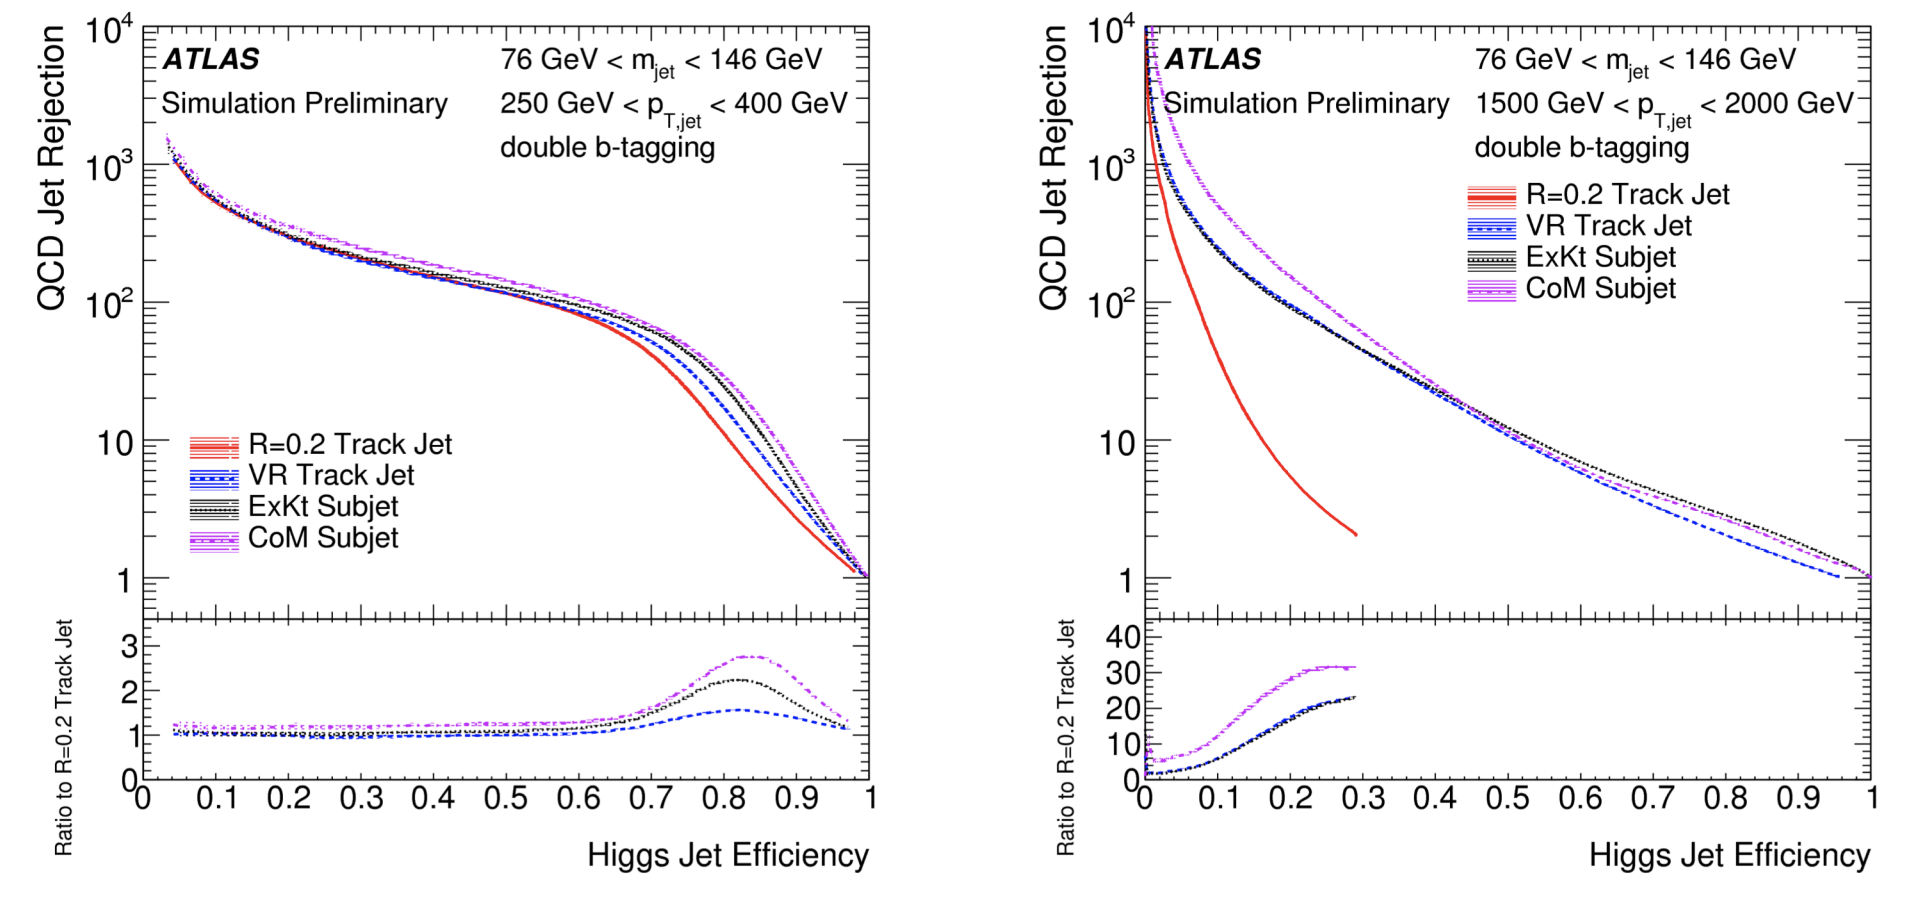
\includegraphics[width=1\textwidth]{chapters/c5/figures/higgs_ROC}

 \end{center}
 \caption{ROC curves using four different subjet techniques: R = 0.2 track jets, VR track jets, ExKt calorimeter jets, and CoM calorimeter jets.}
 \label{fig:higgs_ROC}
\end{figure}
\par The VR track jet technique was chosen to use as subjets in the mono-Higgs analysis as an existing framework to calibrate track jets was readily available in ATLAS.













%\chapter{Boosted Xbb tagging}

Sample text sample text sample text. Sample text sample text sample text.
Sample text sample text sample text. Sample text sample text sample text.
Sample text sample text sample text. Sample text sample text sample text.
Sample text sample text sample text. Sample text sample text sample text.
Sample text sample text sample text.

\section{Sample section}
Sample text sample text sample text. Sample text sample text sample text.
Sample text sample text sample text. Sample text sample text sample text.
Sample text sample text sample text. Sample text sample text sample text.

\subsection{Sample subsection}
Sample text sample text sample text. Sample text sample text sample text.
Sample text sample text sample text. Sample text sample text sample text.
Sample text sample text sample text. Sample text sample text sample text.

\subsection{Sample subsubsection}
Sample text sample text sample text. Sample text sample text sample text.
Sample text sample text sample text. Sample text sample text sample text.
Sample text sample text sample text. Sample text sample text sample text.

\section{Sample section}
Sample text sample text sample text. Sample text sample text sample text.
Sample text sample text sample text. Sample text sample text sample text.
Sample text sample text sample text. Sample text sample text sample text.

\subsection{Sample subsection}
Sample text sample text sample text. Sample text sample text sample text.
Sample text sample text sample text. Sample text sample text sample text.
Sample text sample text sample text. Sample text sample text sample text.

>>>>>>> 794ba0b85cc1ec9527420dfc0c1d19358b25de27
\chapter{Signal selection}

\label{ch:ana-sig}

\par In this analysis, in order to obtain a high signal over background efficiencies, the physics object level selection is applied first, then, signal regions are designed. 
Moreover, control regions are defined to constrain the background contribution.

\section{Physics object definition}
\label{sec:ana-sig:physobj}

\subsection{Leptons}

\begin{itemize}
    \item \textbf{Electrons}: As described in Section~\ref{sec:el}, electrons can be identified using various likelihood-based criteria, for example, shower profile selections, track quality, and high threshold TRT hits. The electron identification criteria that are used in this analysis are listed In Table~\ref{tab:c7:physobj:ele}.
    \item \textbf{Muons}: Muons are reconstructed with combined information from the inner tracker and muon spectrometer. Moreover, two different working points are applied in this analysis for muon identification. A loose criterion is applied as baseline muon selection to obtain larger acceptance, while the medium working point is used in signal selection for higher purity. More details are listed in Table~\ref{tab:c7:physobj:muo}.
    \item \textbf{$\tau$-Leptons}: As decribed in Section~\ref{sec:taus}, $\tau$-lepton is reconstructed using the inner tracker and calorimeter. Since events with $\tau$-leptons are vetoed in both signal and control regions, a loose $\tau$-lepton working point is enough for this analysis. More information can be found in Table~\ref{tab:c7:physobj:tau}.
\end{itemize}

\begin{table}[ht]
    \caption{Electron selection criteria.}
    \label{tab:c7:physobj:ele}
    \centering
    \begin{tabular}{|c|c|}
        \hline
        Feature & Criterion \\
        \hline
        \hline
        Pseudorapidity range & \(|\eta| < 2.47\) \\
        \hline
        Transverse momentum & \pt~$>$ 7~\GeV~\\
        \hline
        Track to vertex association & \(|d_{0}^{\text{BL}}(\sigma)| < 5\)\\ & \(|\Delta z_{0}^{\text{BL}} \sin{\theta}| < 0.5mm\) \\
        \hline
        Identification & \texttt{FCLoose} \\
        \hline
        Isolation & \texttt{LooseTrackOnly / FCHighPtCaloOnly} \\
        \hline
    \end{tabular}
\end{table}

\begin{table}[ht]
    \caption{Muon selection criteria.}
    \label{tab:c7:physobj:muo}
    \centering
    \begin{tabular}[ht]{|c|c|c|}
        \hline
        Feature & Baseline criterion & Signal criterion \\
        \hline
        \hline
        Selection working point & \texttt{Loose} & \texttt{Medium} \\
        \hline
        Isolation working point & \texttt{FCLoose} &  \texttt{FCTightTrackOnly} \\
        \hline
        Momentum calibration & Sagitta correction & Sagitta correction \\
        \hline
        \pt~cut & 7~\GeV~& 7~\GeV~\\ 
        \(|\eta|\) cut & \(< 2.7\) & \(< 2.5\) \\
        \hline
        \(d_{0}\) significance cut & 3 & 3 \\
        \hline
        \(z_{0}\) cut & 0.5mm & 0.5mm \\
        \hline
    \end{tabular}
\end{table}

\begin{table}[ht]
    \caption{Tau selection criteria.}
    \label{tab:c7:physobj:tau}
    \centering
    \begin{tabular}{|c|c|}
        \hline
        Feature & Criterion \\
        \hline
        \hline
        Pseudorapidity range & \(|\eta| < 2.5\) \\
        \hline
        Track selection & 1 or 3 tracks \\
        \hline
        Charge & \(|Q| = 1\) \\
        \hline
        Tau energy scale & \texttt{MVA TES} \\
        \hline
        Transverse momentum & \pt~$>$ 20~\GeV~\\
        \hline
        Jet rejection & BDT-based (\texttt{Loose}) \\
        \hline
        Electron rejection & BDT-based \\
        \hline
        Muon rejection & \specialcell{Via overlap removal in \(\Delta R < 0.2\) and \pt~$>$ 2~\GeV.\\ Muons must not be Calo-tagged} \\
        \hline
    \end{tabular}
\end{table}

\subsection{Jets}

\begin{itemize}
    \item \textbf{Small-radius jets}: As mentioned in Section~\ref{sec:jets}, small-radius jets can be divided into two categories: central jets and forward jets. In this analysis, only the central jets are used to reconstruct the Higgs boson, while both central and forward jets are involved in the \met~calculation. More details about small-radius jet identification can be found in Table~\ref{tab:c7:physobj:srjets}.
    \item \textbf{Large-radius jets}: The large-radius jets are recontructed with large cone size (R=1.0). These large cone size jets are used to reconstruct the boosted Higgs boson. More details are listed in Table~\ref{tab:c7:physobj:lrjets}.
    \item \textbf{Variable-radius track jets}: The variable-radius track jets are reconstructed from the inner tracker data using the anti-$k_{t}$ algorithm. The jet radius is dependent on the jet \pt: $R=\frac{30~\GeV}{p_{T}}$. The variable-radius track jets provide a better acceptance when reconstructing boosted Higgs bosons in this analysis.
    \item \textbf{b-jets}: $b$-tagging is a technology to identify the b-jets, which is applied on central jets to reconstruct the resolved Higgs boson. More detailed information can be found in Table~\ref{tab:c7:physobj:bjets}.
\end{itemize}

\begin{table}[ht]
    \caption{Small-\(R\) jet reconstruction criteria.}
    \label{tab:c7:physobj:srjets}
    \centering
    \begin{tabular}{|c|c|}
        \hline
        Feature & Criterion \\
        \hline
        \hline
        Algorithm & Anti-$k_{t}$ \\
        \hline
        \(R\)-parameter & 0.4 \\
        \hline
        Input constituent & PFlow \\
        \hline
        \texttt{CalibArea} tag & 00-04-82 \\
        \hline
        Calibration configuration & \specialcell{\texttt{JES\_MC16Recommendation\_}\\\texttt{Consolidated\_EMTopo\_Apr2019\_Rel21.config}} \\
        \hline
        Calibration sequence (Data) & \texttt{JetArea\_Residual\_EtaJES\_GSC\_Insitu} \\
        \hline
        Calibration sequence (MC) & \texttt{JetArea\_Residual\_EtaJES\_GSC} \\
        \hline
        Jet cleaning & \texttt{TightBad} \\
        \hline
        \pt~& \(> 20~\GeV\) (central) / \(> 30~\GeV\) (forward) \\
        \hline
        \(|\eta|\) & \(< 2.5\) (central) /  \(2.5 < |\eta| < 4.5 \) (forward) \\
        \hline
        JVT & \specialcell{\texttt{Medium} working point,\\applied only to central jets with \pt~$<$ 120~\GeV} \\
        \hline
    \end{tabular}
\end{table}
    
\begin{table}[ht]
    \caption{Large-\(R\) jet reconstruction criteria.}
    \label{tab:c7:physobj:lrjets}
    \centering
    \begin{tabular}{|c|c|}
        \hline
        Feature & Criterion \\
        \hline
        \hline
        Algorithm & Anti-$k_{t}$ \\
        \hline
        R-parameter & 1.0 \\
        \hline
        Input constituent & \texttt{LCTopo} \\
        \hline
        Grooming algorithm & Trimming \\
        \hline
        Subjet \pt~fraction for trimming & 0.05 \\
        \hline
        \(R_{\text{trim}}\) & 0.2 \\
        \hline
        \texttt{CalibArea} tag & 00-04-82 \\
        \hline
        Calibration configuration (Data) & \specialcell{\texttt{JES\_MC16recommendation\_FatJet}\\\texttt{\_Trimmed\_JMS\_comb\_3April2019.config}} \\
        \hline
        Calibration configuration (MC) & \specialcell{\texttt{JES\_MC16recommendation\_FatJet}\_\\\texttt{Trimmed\_JMS\_comb\_17Oct2018.config}} \\
        \hline
        Calibration sequence (Data) & \texttt{EtaJES\_JMS\_Insitu} \\
        \hline
        Calibration sequence (MC) & \texttt{EtaJES\_JMS} \\
        \hline
        \pt~& \(> 200~\GeV\) \\
        \hline
        \(|\eta|\) & \(< 2\) \\
        \hline
    \end{tabular}
\end{table}

\begin{table}[ht]
    \caption{b-jets selection criteria.}
    \label{tab:c7:physobj:bjets}
    \centering
    \begin{tabular}{|c|c|}
        \hline
        Feature & Criterion \\
        \hline
        \hline
        Jet collection & \texttt{AntiKt4EMPFlow / AntiKtVR30Rmax4Rmin02} \\
        \hline
        Algorithm & \texttt{DL1} \\
        \hline
        Operating point & Eff = 77 \\
        \hline
        CDI & \texttt{2017-21-13TeV-MC16-CDI-2019-07-30\_v1} \\
        \hline
    \end{tabular}
\end{table}
  
\subsection{Missing transverse momentum}

\par As described in Section~\ref{sec:met}, the missing transverse momentum (\met) is defined as the magnitude of the missing transverse momentum vector, which is calculated using all well-reconstructed physics object, like electron, muon and jets. 
More information about the \met~selection for this analysis is listed in Table~\ref{tab:c7:physobj:met}.

\begin{table}[ht]
    \caption{\met~reconstruction criteria.}
    \label{tab:c7:physobj:met}
    \centering
    \begin{tabular}{|c|c|}
        \hline
        Parameter & Value \\
        \hline
        \hline
        Algorithm & Calo-based \\
        \hline
        Soft term & Track-based (TST) \\
        \hline
        \met~operating point & \texttt{Tight} \\
        \hline
    \end{tabular}
\end{table}

\section{Signal regions}
\label{sec:ana-sig:sigreg}
\par Signal regions are a set of phase spaces defined by a combination of selection conditions for signal selection. 
In this analysis, the most important signature is the Higgs boson, which has different signatures at different energy scales. 
Therefore, resolved and merged regions are designed as sub-signal regions to probe signals effectively at different Higgs boson momenta.

\subsection{Common event selection}
\par Several common event selection criteria are applied for both resolved and merged regions as a baseline selection.
\begin{itemize}
    \item \textbf{Event cleaning}: Event cleaning applies a set of filters to veto corrupted or noisy events. In this analysis, LAr noise burst, tile corruption, SCT recovery procedure and incomplete events are applied as the event cleaning filters. More information can be found in Ref~\cite{c8-evt-cleaning}.
    \item \textbf{Loose jet Veto}: In analysis, reconstructed jets can due to noise, collision background, etc.. The TightBadJet criterion, provided by the Jet/\met~group, is applied in this analysis to veto events that contain fake jets.
    \item \textbf{\met~selection}: In signal regions, a constraint \met~$>$150~\GeV~is applied. In control regions, the lepton momentum is treated as part of the missing transverse momentum and the same \met~cut is applied.
    \item \textbf{Light lepton and $\tau$-lepton veto}: Events that contain a electron, muon or $\tau$-lepton, as defined in Section~\ref{sec:ana-sig:physobj}, are rejected.
    \item \textbf{Extended $\tau$-lepton veto}: An extended $\tau$ veto is applied in case a $\tau$-lepton failed to be identified. A hadronically decayed $\tau$ can be viewed as a jet. Therefore, a jet is considered as a $\tau$ candidate if it fullfills two conditions: (1) The track multiplicity in the jet cone is between 1 and 4. (2) The azimuthal separation between the jet and \met~is $\Delta \phi \leq 22.5^\circ$. The cut on the track multiplicity in the jet cone makes sure that the hadronic decay products in the jet are compatible with $\tau$-lepton decay products, namely with charged pions. The tracks considered are required to be associated with the primary vertex and have \pt~greater than 1 ~\GeV. The cut on the angular separation between the jet and \met~selects $\tau$-candidates that come from W bosons.
    \item \textbf{$\min_{j \in \{1,2,3\}}\Delta\phi(E_{\mathrm{T}}^{\mathrm{miss}},j)$ selection}: QCD multijet events can pass the \met~requirement because of jet energy mis-measurement. In case of fake \met, the \met~will generally point in the direction of leading jets. Therefore, an angular cut between \met~and leading jets is applied to veto these events.
\end{itemize}

\par After this baseline selection, the signal regions need to be analyzed different sub-regions based on the Higgs boson signature. 
In the target model, the sum of the \met~vector and Higgs boson transverse momentum vector should be zero based on momentum conservation. 
Therefore, one can apply a single cut on \met~to separate events with resolved or merged Higgs bosons. In this analysis, the cut \met~$<$500~\GeV~selects the resolved region while \met$>$500~\GeV~defines the merged region. Higgs boson identification, which will be detailed in the rest of this section, is different in these two signal regions.
\par Moreover, there is one additional condition to select events with at least one b-jet. $b$-tagging is applied on all small-radius central jets in the resolved region, but only on the two leading track jets that are associated to large-radius jets in the merged region.

\subsection{Resolved region}

\par In the resolved region, the Higgs boson momentum is relatively low. Therefore, the Higgs boson decay products, two $b$-jets, can be resolved into two separate jets. To reconstruct the Higgs boson, a set of jet candidates needs to be selected first. There are two categories in the Higgs boson jet candidate set: (1) $b$-tagged jets, (2) central non $b$-tagged jets. The jets are ordered in decreasing transverse momentum within each category. The first two from each set of jets (referred as j1 and j2 below) are used to reconstruct the Higgs boson candidate, which is referred as $H_{reco}$.

\par There are several criteria to select the Higgs boson in the resolved channel:

\begin{itemize}
    \item \textbf{\pt~of $H_{reco}$}: This is expected to increase with \met. Therefore, a selection \pt$(H_{reco})>$100~\GeV~is applied when \met~$<$~350~\GeV, while \pt$(H_{reco}) >$~300~\GeV~is required when 
        350~\GeV~$<$~\met~$<$ 500~\GeV.
    \item \textbf{$m_{jj}$}: A window around the mass of the reconstructed Higgs boson is helpful to identify the Higgs boson. The mass of the reconstructed Higgs boson can be calculated from the invariant mass of the jet pair ($m_{jj}$) that forms $H_{reco}$. A window 50~\GeV~$< m_{jj} <$ 280~\GeV~is applied in this analysis. 
    \item \textbf{$m_{T}^{b}$}: In the resolved region, the major background is top quark pair production. $m_{T}^{b}$ is introduced to reject these background events. $m_{T}^{b}$ is defined as: $m_{T}^{b}=\sqrt{2p_{T}^{b}E_{T}^{miss}(1-cos\Delta\phi(\vec{p}_{T}, \vec{E}_{T}^{miss}))}$. $m_{T}^{b}$ is calculated using the $b$-jets that are closest to and furthest from \met. The closest $b$-jet $m_{T}^b$ is required to be greater than 170~\GeV, while the furthest must be greater than 200~\GeV.
\end{itemize}

\par In addition, it is possible that the measured \met~of an event is due to a resolution fluctuation. Therefore, a \met~significance cut $S > 12$ is introduced to reject fake \met~events.

\subsection{Merged region}

\par In the merged region, the momentum of the Higgs boson is relatively high, and therefore, the decay products are close to each other in the lab frame and can be merged into a single cone, which is reconstructed as a large-radius jet in detector.
\par Several criteria are applied on the large-radius jet to identify the Higgs boson in the merged region:
\begin{itemize}
    \item \textbf{$m_{J}$}: The invariant mass of the large-radius jet is an expression of Higgs boson mass. A window 50~\GeV $< m_{J} <$ 270~\GeV~is applied.
    \item \textbf{Variable-radius track jets association}: At least two variable-radius track jets need to be associated to the large-radius jet.
\end{itemize}

\par As a summary of Section~\ref{sec:ana-sig:sigreg}, both resolved and merged signal region selections are listed in Table~\ref{tab:c7:sigreg:summary}.

\begin{table}[h]
    \centering
	\begin{center}
        \begin{tabular}{cc}
            \hline
            \textbf{Resolved} & \textbf{Merged} \\
            \hline
            \hline
            \multicolumn{2}{c}{lowest unprescaled \met~trigger} \\
            \hline
            \multicolumn{2}{c}{veto on baseline light leptons and $\tau$-leptons} \\
            \hline
            \multicolumn{2}{c}{extended $\tau$-veto} \\
            \hline
            \multicolumn{2}{c}{\met~$>$ 150~\GeV} \\
            \hline
            \multicolumn{2}{c}{$\mindphi > 20^\circ$} \\
            \hline
            \met~$<$ 500~\GeV~& \met~$>$ 500~\GeV~\\
            \hline
            N(central small-R jets) $\geq$ 2 & N(central large-R jets) $\geq$ 1 \\
            \hline
            N($b$-tagged small-R jets) $\geq 1$ & N($b$-tagged associated track jets) $\geq 1$ \\
            \hline
            S $>$ 12 & --- \\
            \hline
            \pt$(jj) >$ 100~\GeV~if \met~$<$ 350~\GeV~& --- \\
            \hline
            \pt$(jj) >$ 300~\GeV~if \met~$\geq$ 350~\GeV~& --- \\
            \hline
            $\mtb{\min} >$ 170~\GeV& --- \\
            \hline
            $\mtb{\max} >$ 200~\GeV& --- \\
            \hline
            50~\GeV~$< m_{jj} <$ 280~\GeV~& 50~\GeV~$< m_{J} <$ 270~\GeV~\\
            \hline
            $b$-tagging on small-radius jets & $b$-tagging on variable-radius track jets \\
            \hline
		\end{tabular}
	\end{center}
	\caption{Summary of the resolved and merged event selections applied in the 0-lepton channel. $\mathcal{S}$ denotes the object based \met~significance.}
	\label{tab:c7:sigreg:summary}
\end{table}

\section{Control regions}
\label{sec:ana-sig:ctlreg}
\par Control regions are a set of phase spaces that are orthogonal to the signal regions. 
Control regions are designed to validate the backgrounds estimate in the signal regions.

\subsection{1-lepton control region}
\par In the signal region the W + jets background is mostly composed of events in which the $W$-boson decays leptonically. 
The $t\bar{t}$ background in the signal region originates almost completely from semileptonic $t\bar{t}$ decays. 
Events with leptons can enter the signal region if the leptons fail to be identified or if they are outside the detector acceptance. 
The largest contribution comes from decays involving $\tau$-leptons, as shown in Figure~\ref{fig:ttbarDecayCat}. 
Figure~\ref{fig:ttbarDecayCatKinematic} shows the distributions of different kinematic variables for the dominant decay modes. 
From these it can be seen that shapes of the event variables agree well within the statistical uncertainties. 
Therefore the W+jets and $t\bar{t}$ backgrounds can be estimated using a 1-lepton control region, in which the lepton could have any flavor in principle.

\begin{figure}[h]
    \centering
    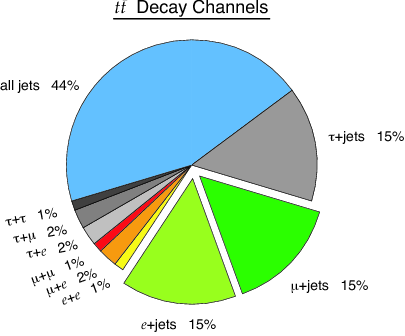
\includegraphics[width=0.9\textwidth]{chapters/c7/figures/ttbar-decay-modes.png}
    \caption{Decay categories for $t\bar{t}$ events. The classification of the decay processes was performed by examining the truth particle information within the reconstructed signal region events. The three dominant decay modes are the semileptonic decays with either a light lepton, a leptonically or a hadronically decaying $\tau$-lepton.}
    \label{fig:ttbarDecayCat}
\end{figure}

\begin{figure}[h]
    \centering
	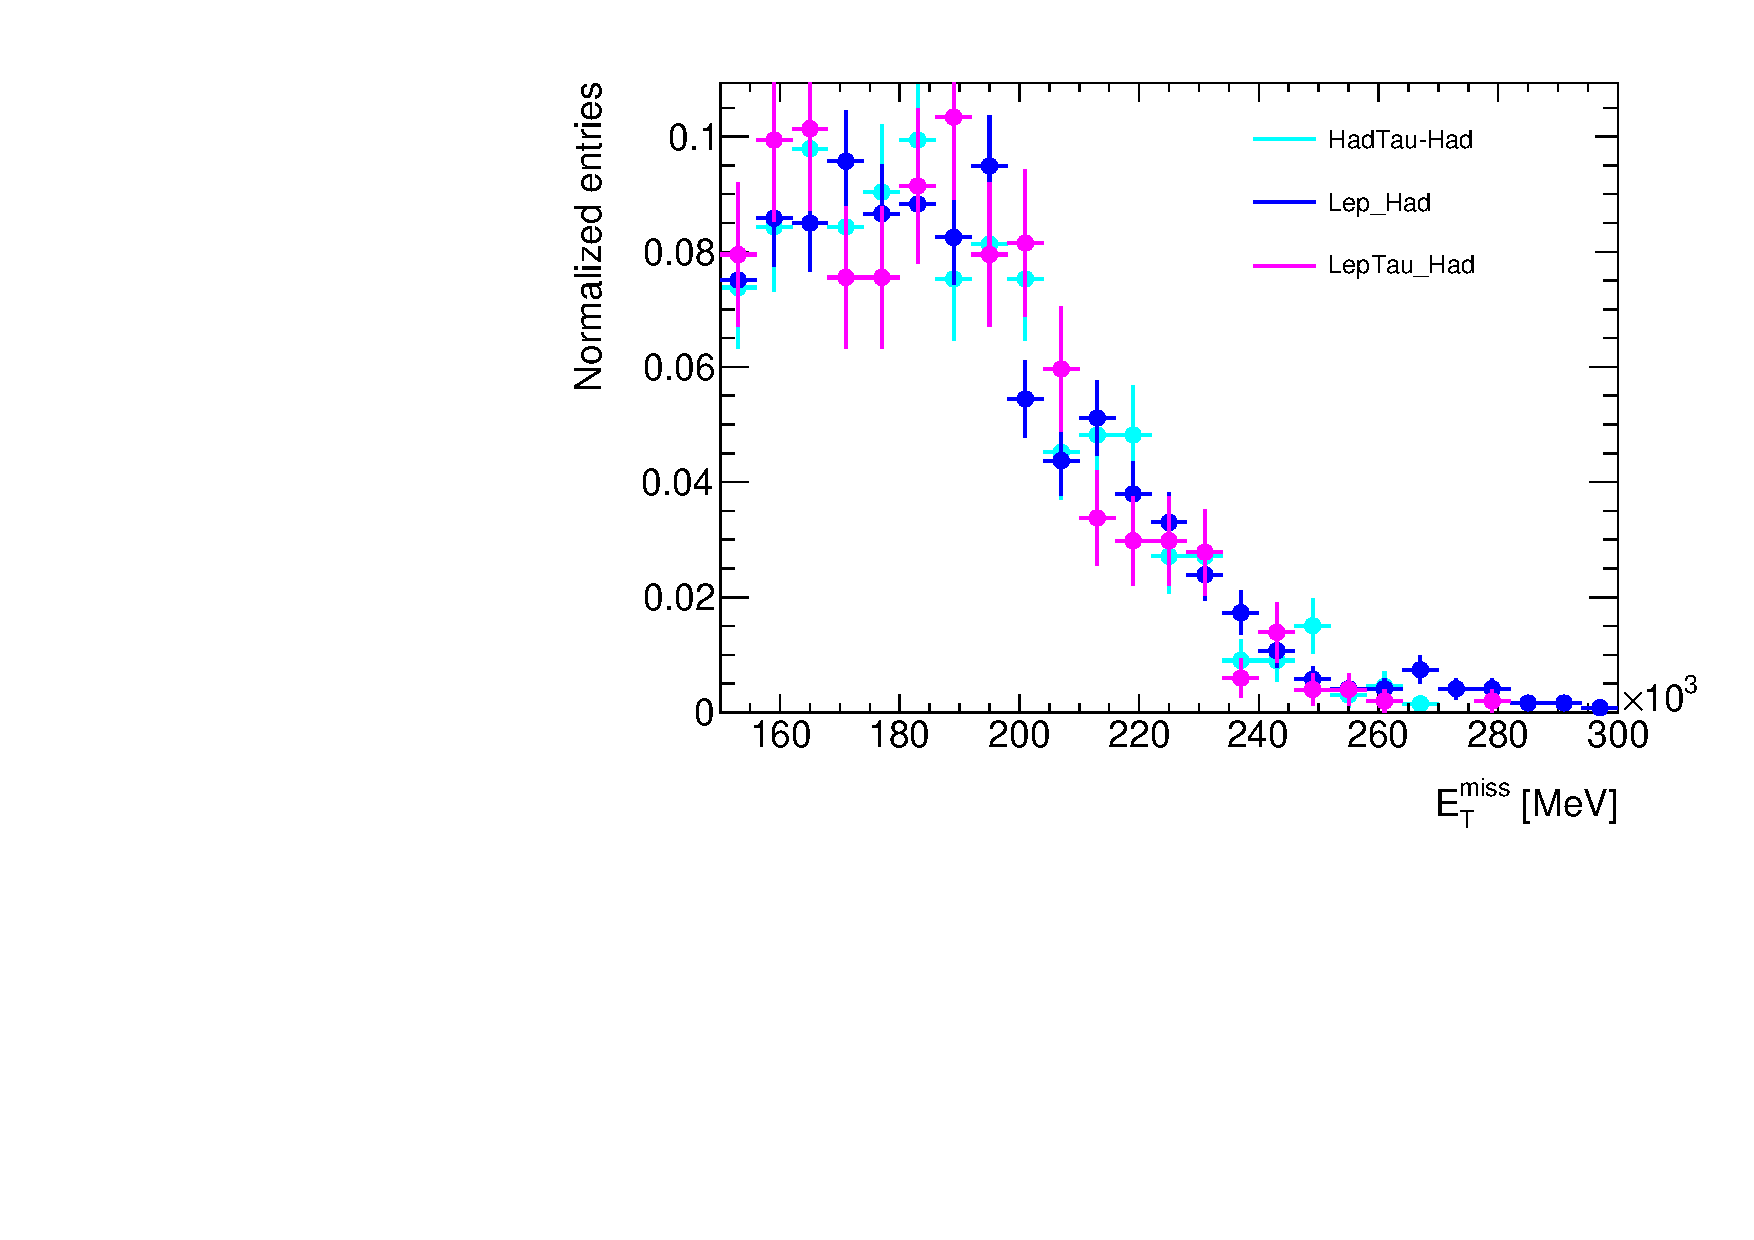
\includegraphics[width=0.45\textwidth]{chapters/c7/figures/ttbar_MetTST_met.pdf}
	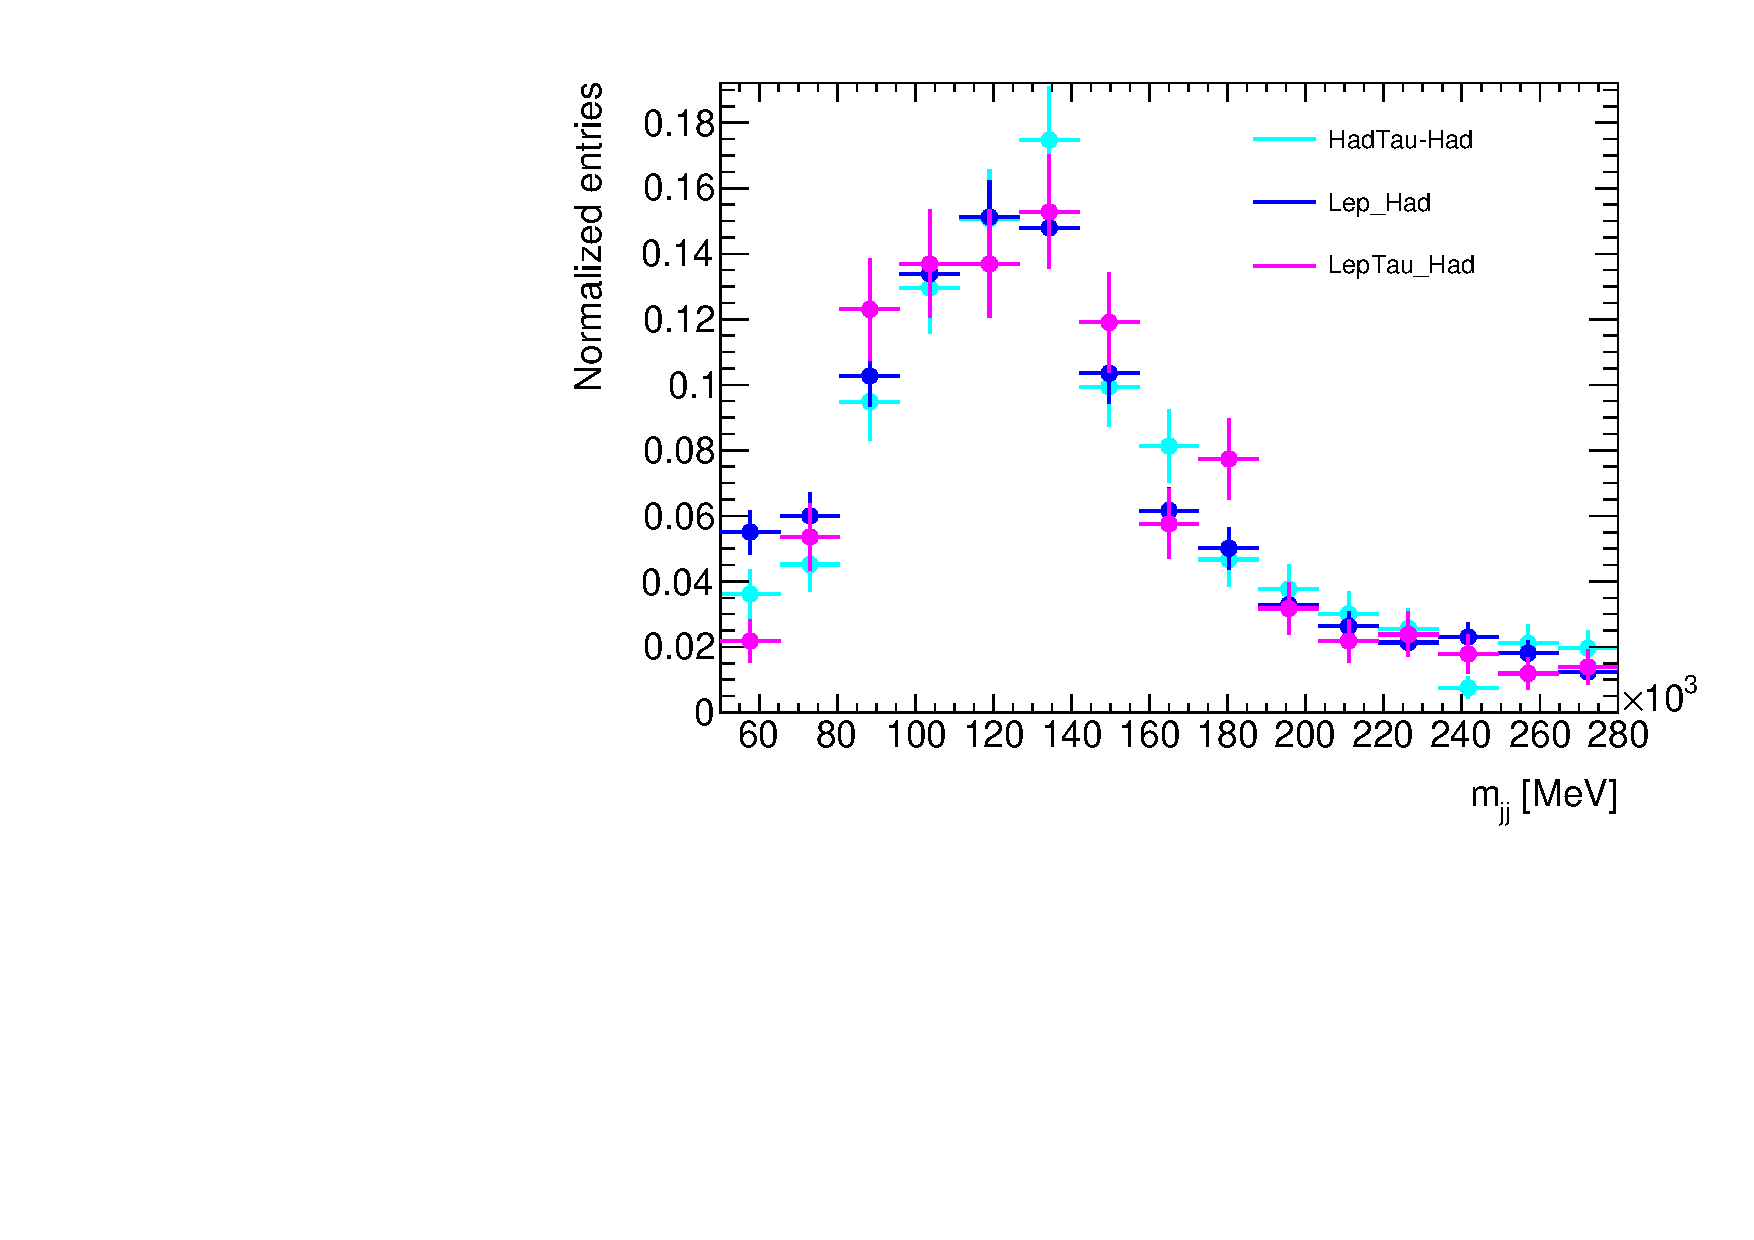
\includegraphics[width=0.45\textwidth]{chapters/c7/figures/ttbar_m_jj.pdf}
	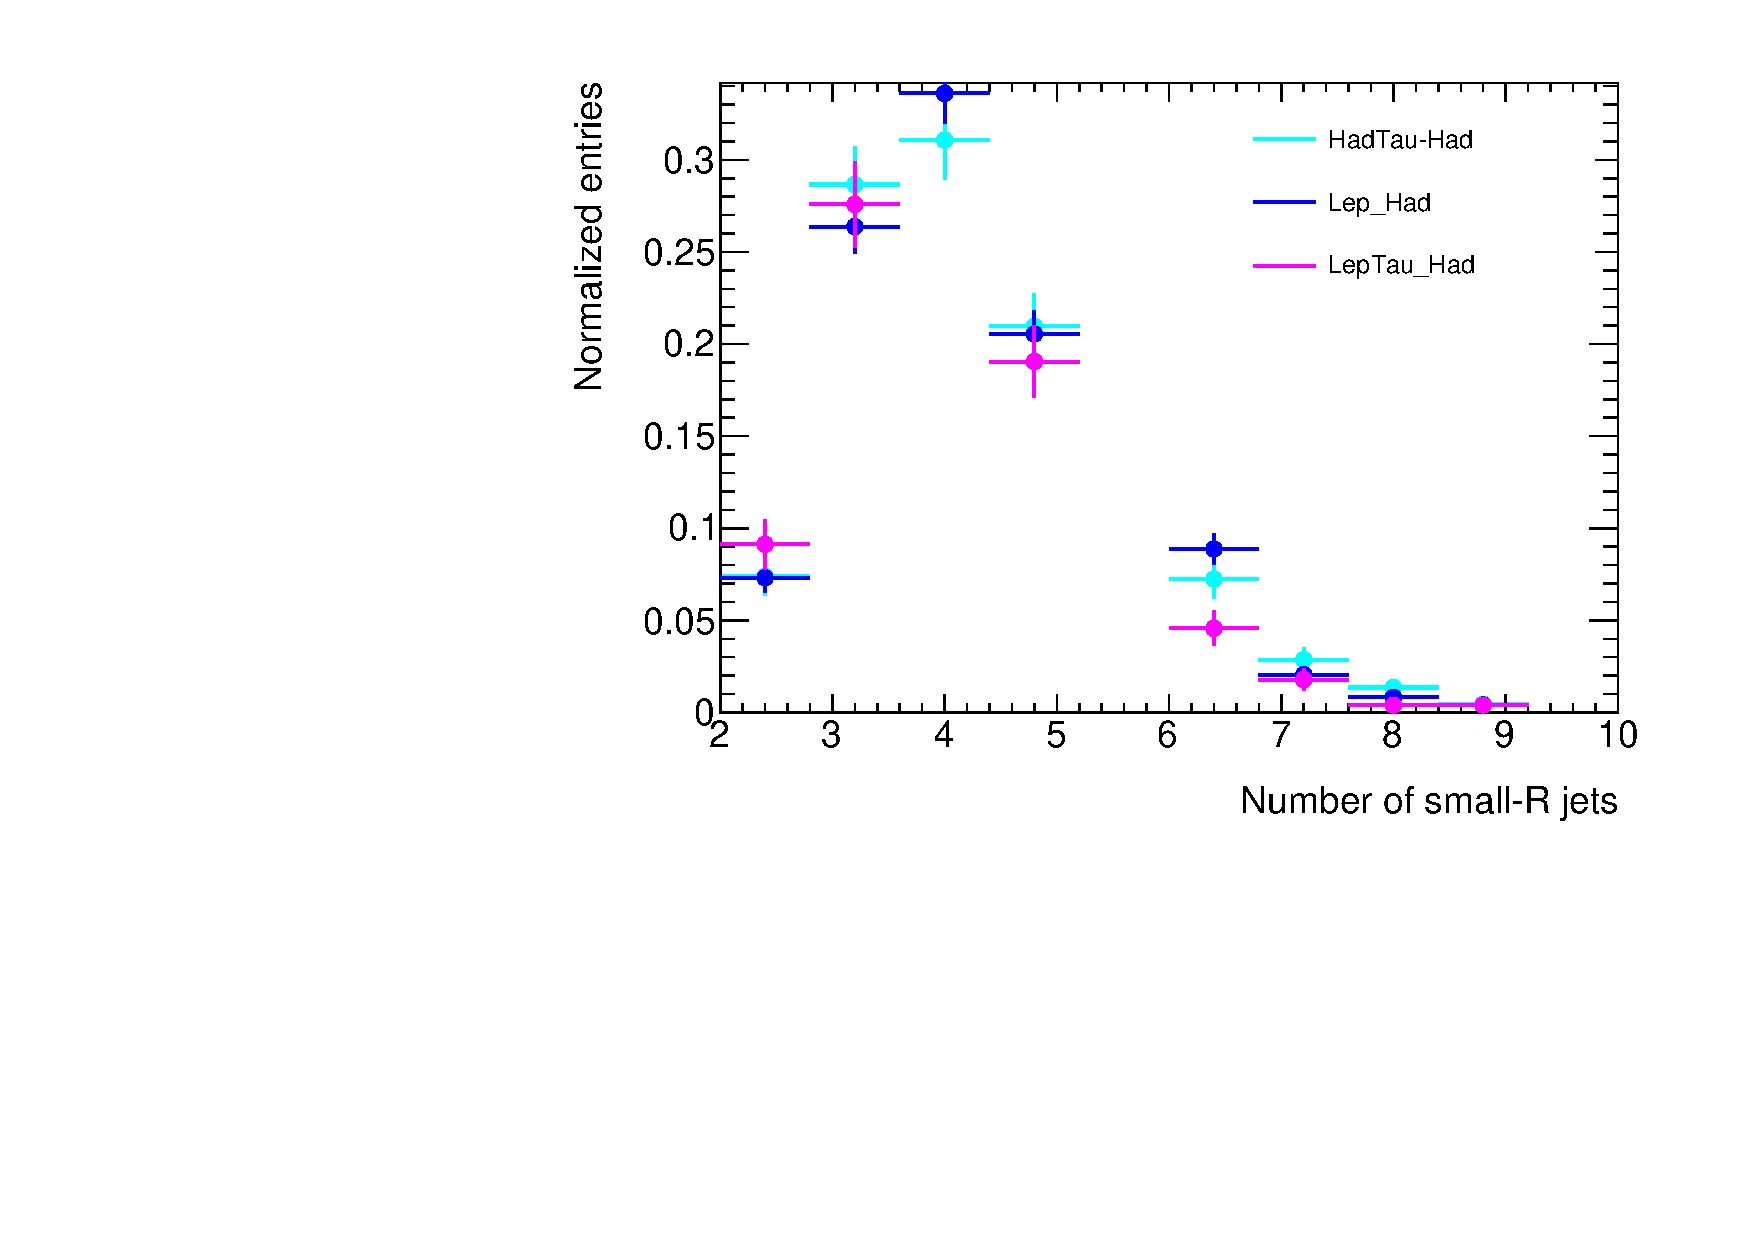
\includegraphics[width=0.45\textwidth]{chapters/c7/figures/ttbar_N_Jets04.pdf}		
	\caption{Normalised distributions of \met, the Higgs boson candidate mass and the number of small-radius jets for $t\bar{t}$ events. The distributions are shown separately for the three semileptonic decay modes, which are the dominant decays modes in the signal region.}
	\label{fig:ttbarDecayCatKinematic}
\end{figure}

\par The 1-muon control region is chosen to constrain W + jets related background. Events in this control region is required to have exactly one muon and no other baseline leptons.

\subsection{2-lepton control region}
\par A 2-lepton control region is used to estimate the Z +jets background. 
In the signal region the $Z(\to\nu\nu)+jets$ production leads to a significant amount of background, which has the topology as $Z(\to\ell\ell)+jets$, because the momentum of the $Z$ boson does not depend on its decay products. 
Hence the normalisation of $Z(\to\nu\nu)+jets$ events can be estimated with the help of a $Z(\to\ell\ell)+jets$ control region.

\par The 2-lepton control region is defined by selecting exactly two muons or two electrons. 
At least one of the leptons needs to saitisfy the signal lepton criteria with sufficiently high \pt~to pass the trigger. 
The leading muon is required to have \pt~$>$ 25~\GeV, while the leading electron is \pt~$>$ 27~\GeV. 
The other lepton is not required to pass the signal lepton selection to increase the acceptance. 
Moreover, since the two leptons originate from a $Z$ boson, a mass window requirement is implemented to identify the $Z$ mass peak: $|m_{Z}-m_{ll}|$ $<$ 10~\GeV.

\chapter{Systematic uncertainties}
\label{ch:sys-unc}

\par Once signal regions are determined, one can use the data observations and their systematic uncertainties to perform statistical analysis. 
In this analysis, both experimental and theoretical uncertainties are considered.

\section{Experimental systematic uncertainties}

\par Experimental uncertainties arise from the reconstruction of physics objects, reflecting uncertainties related to detectors or reconstruction algorithms performance. 
Multiple physical objects, like muons, electrons, jets, \met, etc., are used in this analysis. 
Therefore, the systematic uncertainties of the reconstruction of these objects need to be considered carefully when interpreting the analysis result. A summary of these experimental uncertainties can be viewed in Tables~\ref{tab:c8:expsyst1}, ~\ref{tab:c8:expsyst2} and ~\ref{tab:c8:expsyst3}.

\begin{table}[h]
    \scriptsize
    \begin{center}
        \begin{tabular}{ll}
            \hline
            \hline
            Systematic uncertainty & Short description \\
            \hline
            \multicolumn{2}{c}{\textbf{Event}} \\
            \hline
            Luminosity & Uncertainty on the total integrated luminosity \\
            \hline
            \multicolumn{2}{c}{\textbf{Electrons}} \\
            \hline
            EL\_EFF\_Trigger\_TOTAL\_1NPCOR\_PLUS\_UNCOR & Trigger efficiency uncertainty \\
            EL\_EFF\_Reco\_TOTAL\_1NPCOR\_PLUS\_UNCOR & Reconstruction efficiency uncertainty \\
            EL\_EFF\_ID\_TOTAL\_1NPCOR\_PLUS\_UNCOR & ID efficiency uncertainty \\
            EL\_EFF\_Iso\_TOTAL\_1NPCOR\_PLUS\_UNCOR & Isolation efficiency uncertainty \\
            EG\_SCALE\_ALL & Energy scale uncertainty \\
            EG\_RESOLUTION\_ALL & Energy resolution uncertainty \\
            \hline
            \multicolumn{2}{c}{\textbf{Muons}} \\
            \hline
            mu20\_iloose\_L1MU15\_OR\_HLT\_mu40\_MUON\_EFF\_Trig & Trigger efficiency uncertainties \\ 
			mu24\_ivarmed\_OR\_HLT\_mu40\_MU\_EFF\_TrigStat & None \\ 
			mu24\_ivarmed\_OR\_HLT\_mu50\_MU\_EFF\_TrigStat & None \\ 
			mu26\_ivarmed\_OR\_HLT\_mu50\_MU\_EFF\_TrigStat & None \\ 
            MUON\_EFF\_RECO\_STAT & Reconstruction uncertainty for \pt~$>15GeV$ \\
            MUON\_EFF\_RECO\_SYS & None \\ 
			MUON\_EFF\_RECO\_STAT\_LOWPT & \speciallcell{Reconstruction and \\ID efficiency uncertainty for \pt~$<15GeV$} \\ 
			MUON\_EFF\_RECO\_SYS\_LOWPT & None \\ 
			MUON\_ISO\_STAT & Isolation efficiency uncertainty \\ 
			MUON\_ISO\_SYS & None \\ 
			MUON\_TTVA\_STAT & Track-to-vertex association efficiency uncertainty \\ 
			MUON\_TTVA\_SYS & None \\ 
            MUONS\_SCALE & Energy scale uncertainty \\
            MUONS\_SAGITTA\_RHO & Variations in the scale of the momentum \\
            MUONS\_SAGITTA\_RESBIAS & Variations in the scale of the momentum \\
            MUONS\_ID & Energy resolution uncertainty from inner detector \\
            MUONS\_MS & Energy resolution uncertainty from muon system \\
            \hline
            \multicolumn{2}{c}{\textbf{\met~related}} \\
            \hline
            METTrigStat & Trigger efficiency uncertainty \\
            METTrigSyst & None \\
            MET\_SoftTrk\_ResoPerp & \speciallcell{Track-based soft term related to \\transversal resolution uncertainty} \\ 
			MET\_SoftTrk\_ResoPara & \speciallcell{Track-based soft term related to \\longitudinal resolution uncertainty} \\
			MET\_SoftTrk\_Scale & \speciallcell{Track-based soft term related to \\longitudinal scale uncertainty} \\
			MET\_JetTrk\_Scale  & \speciallcell{Track \met~scale uncertainty \\due to tracks in jets} \\
            PRW\_DATASF & \speciallcell{Uncertainty on data scale factor used \\for the computation of pileup reweighting} \\
            \hline
            \hline
		\end{tabular}
	\end{center}
	\caption{A summary of the experimental systematic uncertainties.}
	\label{tab:c8:expsyst1}
\end{table}

\begin{table}[h]
    \scriptsize
    \begin{center}
        \begin{tabular}{ll}
            \hline
            \hline
            Systematic uncertainty & Short description \\
            \hline
            \multicolumn{2}{c}{\textbf{Small-radius jets}} \\
            \hline
            JET\_EtaIntercalibration\_Modelling & $\eta$-intercalibration: MC generator modelling uncertainty \\
            JET\_EtaIntercalibration\_TotalStat & $\eta$-intercalibration: statistical uncertainty \\
            JET\_EtaIntercalibration\_NonClosure\_highE & \speciallcell{$\eta$-intercalibration: non-closure uncertainty \\of jet response, high energy component} \\
            JET\_EtaIntercalibration\_NonClosure\_negEta & \speciallcell{$\eta$-intercalibration: non-closure uncertainty \\of jet response, negative $\eta$ component} \\
            JET\_EtaIntercalibration\_NonClosure\_posEta & \speciallcell{$\eta$-intercalibration: non-closure uncertainty \\of jet response, positive $\eta$ component} \\
            JET\_Pileup\_OffsetMu & Pileup: Offset, term for number of interactions per crossing $\mu$ \\
            JET\_Pileup\_OffsetNPV & Pileup: Offset, term for number of primary vertices \\
            JET\_Pileup\_PtTerm & Pileup: Offset, \pt~term \\
            JET\_Pileup\_RhoTopology & Pileup: Offset, $\rho$ topology uncertainty on jet areas \\
            JET\_Flavor\_Composition & Flavor composition uncertainty \\
            JET\_Flavor\_Response &  Flavor response uncertainty (dominated by gluon response) \\
            JET\_PunchThrough\_MC16 & Punch-through correction uncertainty \\
            JET\_EffectiveNP\_Statistical & \speciallcell{Statistical components of effective jet energy scale uncertainties, \\split into 6 components} \\
            JET\_EffectiveNP\_Modelling & \speciallcell{Modelling components of effective jet energy scale uncertainties, \\split into 4 components} \\
            JET\_EffectiveNP\_Detector & \speciallcell{Detector components of effective jet energy scale uncertainties, \\split into 2 components} \\
            JET\_EffectiveNP\_Mixed & \speciallcell{Effective jet energy scale uncertainties coming from various sources, \\split into 3 components} \\
            JET\_SingleParticle\_HighPt & Uncertainty related to high \pt~jets \\
            JET\_RelativeNonClosure\_MC16 & Closure of the calibration, relative to MC12a \\
            JET\_BJES\_Response & Jet energy scale uncertainty for $b$-jets \\
            JET\_JER\_DataVsMC\_MC16 & \speciallcell{Nuisance parameter covering when jet energy resolution \\in data smaller than resolution in MC} \\
            JET\_JER\_EffectiveNP & Effective jet energy resolution uncertainty; split into 6 components \\
            FT\_EFF\_EIGEN\_B & $b$-tagging efficiency uncertainties ("BTAG\_MEDIUM) \\
            FT\_EFF\_EIGEN\_C & None \\
            FT\_EFF\_EIGEN\_L & None \\
            FT\_EFF\_EIGEN\_extrapolation & $b$-tagging efficiency uncertainty on the extrapolation on high \pt-jets \\
            FT\_EFF\_EIGEN\_extrapolation\_from\_charm & $b$-tagging efficiency uncertainty on $\tau$-jets \\
            \hline
            \hline
        \end{tabular}
	\end{center}
	\caption{A summary of the experimental systematic uncertainties.}
	\label{tab:c8:expsyst2}
\end{table}

\begin{table}[h]
    \scriptsize
    \begin{center}
        \begin{tabular}{ll}
            \hline
            \hline
            Systematic uncertainty & Short description \\
            \hline
            \multicolumn{2}{c}{\textbf{Large-radius jets}} \\
            \hline
            JET\_EtaIntercalibration\_Modelling & $\eta$-intercalibration: MC generator modelling and method uncertainty \\
            JET\_EtaIntercalibration\_R10\_TotalStat & $\eta$-intercalibration: statistical uncertainty \\
            JET\_Flavor\_Composition & Flavor composition uncertainty \\
            JET\_Flavor\_Response & Flavor response uncertainty (dominated by gluon response) \\
            JET\_EffectiveNP\_R10\_Statistical & \speciallcell{Statistical components of effective jet energy scale uncertainties, \\split into 6 components} \\
            JET\_EffectiveNP\_R10\_Modelling & \speciallcell{Modelling components of effective jet energy scale uncertainties, \\split into 4 components} \\
            JET\_EffectiveNP\_R10\_Detector & \speciallcell{Detector components of effective jet energy scale uncertainties, \\split into 2 components} \\
            JET\_EffectiveNP\_R10\_Mixed & \speciallcell{Effective jet energy scale uncertainties coming from various sources, \\split into 3 components} \\
            JET\_SingleParticle\_HighPt & Uncertainty related to high \pt~jets (for R=0.4) \\
            JET\_CombMass\_Baseline	& \speciallcell{Baseline uncertainty of the jet mass scale \\accounting for data-MC differences} \\
            JET\_CombMass\_Modelline & \speciallcell{Modelling uncertainty of the jet mass scale \\accounting for different MC generators} \\
            JET\_CombMass\_Tracking	& \speciallcell{Uncertainty of the jet mass scale accounting \\for tracking variations; 3 variations in total} \\
            \hline
            \multicolumn{2}{c}{\textbf{Variable-radius track jets}} \\
            \hline
            FT\_EFF\_EIGEN\_B & $b$-tagging efficiency uncertainties \\
            FT\_EFF\_EIGEN\_C & None \\
            FT\_EFF\_EIGEN\_L & None \\
            FT\_EFF\_EIGEN\_extrapolation & $b$-tagging efficiency uncertainty on the extrapolation on high \pt-jets \\
            FT\_EFF\_EIGEN\_extrapolation\_from\_charm & $b$-tagging efficiency uncertainty on $\tau$-jets \\
            \hline
            \hline
        \end{tabular}
	\end{center}
	\caption{A summary of the experimental systematic uncertainties.}
	\label{tab:c8:expsyst3}
\end{table}

\section{Theoretical systematic uncertainties}

\par Theoretical uncertainties are due to Monte-Carlo simulation of background and signal processes. 
In this analysis, both the signal and background yields come from Monte-Carlo simulated samples rather than data driven estimation from control regions. 
Therefore, a careful estimation of theoretical uncertainties is needed.

\par The sources of theoretical uncertainty are listed below:

\begin{itemize}
    \item \textbf{Missing higher orders in the calculation of the inclusive matrix elements}: For all processes the calculation of the cross-section relies on a perturbative expansion of the scattering matrix, which is truncated at a certain order. The effect of the missing higher orders is estimated by varying the renormalisation and factorisation scales ($\mu_R$ and $\mu_F$) independently by a factor of 2, excluding the $(\mu_R,\mu_F)=(\frac{1}{2},2),(2,\frac{1}{2})\times \mu_{\text{central}}$ variations, which may lead to large logarithms. 
    \item \textbf{Uncertainties from the choice of PDFs and $\alpha_s$}: This kind of uncertainty arises from uncertainties in the experimental measurements that are used to determine the PDF sets used in each calculation, uncertainties from the choice of the functional form used in the PDF fits, and uncertainties associated to the experimental determination of $\alpha_s$. These are estimated using the PDF4LHC prescription\cite{Butterworth_2016}.
    \item \textbf{Merging scale uncertainties}: For samples generated by merging matrix elements (ME) corresponding to different multiplicities, e.g. $V+jets$, an uncertainty related to the choice of the merging scale, i.e. the scale that separates soft from hard jets, is evaluated by varying the merging scale by a factor of 2 up and down.
    \item \textbf{Resummation scale uncertainties}: For \textsc{Sherpa}\cite{Gleisberg_2009} samples an additional uncertainty is related to the energy cut-off for the integration of MC counterterms in the parton shower (PS).
    \item \textbf{Matching uncertainties}: For samples generated using a NLO matrix element and matched to a parton shower, a comparison between \textsc{Powheg} and \textsc{MG5aMC} is used to probe uncertainties related to the ME/PS matching procedure.
    \item \textbf{Parton shower/Hadronisation uncertainties}: Uncertainties related to algorithmic or parametric differences in the modelling of the PS and hadronisation can be assessed by comparing samples generated with different showering/hadronisation (SHG) generators, typically \textsc{Pythia~8} and \textsc{Herwig~7}.  
    \item \textbf{Eigentune uncertainties}: These are due to uncertainties in the choice of the free parameters that are used in the SHG (shower and hadronisation event generator) program, derived so as to encompass the data used in the ATLAS tuning program\cite{ATL-PHYS-PUB-2014-021}.
    \item \textbf{Other implementation-specific uncertainties}: The variation of the $h_{\text{damp}}$ scale in the \text{Powheg} samples, etc..
\end{itemize}

\par The sources mentioned above are considered and grouped into Monte-carlo templates, which are used as an input of the likelihood fit. There are four types of uncertainties considered in the statistical interpretation:

\begin{enumerate}
    \item \textbf{Inclusive cross-section uncertainties}: Inclusive cross-section uncertainties are implemented in the fit using Gaussian priors that affect the normalisation of a given sample in all regions in a correlated manner (\texttt{OverallSys} in the \textsc{HistFactory} terminology \cite{Cranmer:1456844}). These uncertainties are applied only on the samples whose normalisation is not freely floating in the fit.
    \item \textbf{Shape uncertainties}: Shape uncertainties are uncertainties on the shape of the fitted discriminant ($m(b\bar{b})$). These uncertainties are estimated by comparing the shape of the fitted variables for the nominal MC samples and the alternative samples that probe the uncertainties mentioned as sources of theoretical uncertainties. A comparison of the $m(b\bar{b})$ distribution between the nominal and the alternative MCs provides additional templates (histograms) that define the $\pm1\sigma$ variations (\texttt{HistoSys} in the \textsc{HistFactory} terminology)
    \item \textbf{Relative acceptance uncertainties}: The theory uncertainties can also alter the shape of the observables used to separate the different fit regions. These shape differences induce normalisation/acceptance differences between the regions that are used in the fit. For example, differences in the \met~shape can induce relative acceptance differences between the adjacent \met~bins and differences in the lepton \pt~spectrum can induce relative acceptance differences between the 0 and 1-lepton channels. These are included in the fit as Gaussian priors (\texttt{OverallSys}) whose magnitude is estimated by
    \begin{equation}
    \sigma_{\text{accept}}=\sqrt{\sum_i \left( 1 - \left. \frac{N_A^{\text{alt},i}}{N_B^{\text{alt},i}} \middle/ \frac{N_A^{\text{nom}}}{N_B^{\text{nom}}} \right. \right)^2},
    \end{equation}
    where $i$ runs over all alternative MC generators considered for a given process and $(A,B)=$(SR,CR1), (CR1,CR2), (\met~bin1, \met~bin2), (\met~bin2, \met~bin3), (resolved, merged). Since the uncertainty is relative between region $A$ and region $B$ it is only applied on region $B$ in the fit.
    \item \textbf{Flavour composition uncertainties}: An additional uncertainty on the flavour composition is assigned to the $W$ and $Z$+heavy flavour components ($Zhf, Whf$), which consist of $bb,cc,bc,bl$, in order to allow the $cc,bc,bl$ components to vary separately from the total $Zhf, Whf$ normalisation which is freely floating in the fit.
\end{enumerate}

%\subsection{Signal processes}

%\subsection{Top related processes}

%\subsection{V+jets processes}

%\subsection{Diboson processes}

\section{Data-MC comparison}

\par After obtaining the data and Monte-Carlo simulation yields and evaluating the systematic uncertainties, data and simulation are compared as an important validation of the analysis. 
The data-MC comparison performed in the control regions and the signal region outside the Higgs mass window. 
The results are shown for several physics variables, which are used in this analysis, in both signal regions and control regions. 
One can view the signal regions comparison in $m_{jj}$ or $m_{J}$ in Figure~\ref{fig:data-mc-0l-mjj-2b} and Figure~\ref{fig:data-mc-0l-mjj-3+b}, 1-lepton control region comparison for muon charge in Figure~\ref{fig:data-mc-1l-mu-charge-2b} and Figure~\ref{fig:data-mc-1l-mu-charge-3+b}, and 2-lepton control region comparison for the number of b-jets in Figure~\ref{fig:data-mc-2l-ll-nb-2b} and Figure~\ref{fig:data-mc-2l-ll-nb-3+b}.

\begin{figure}[!htb]
    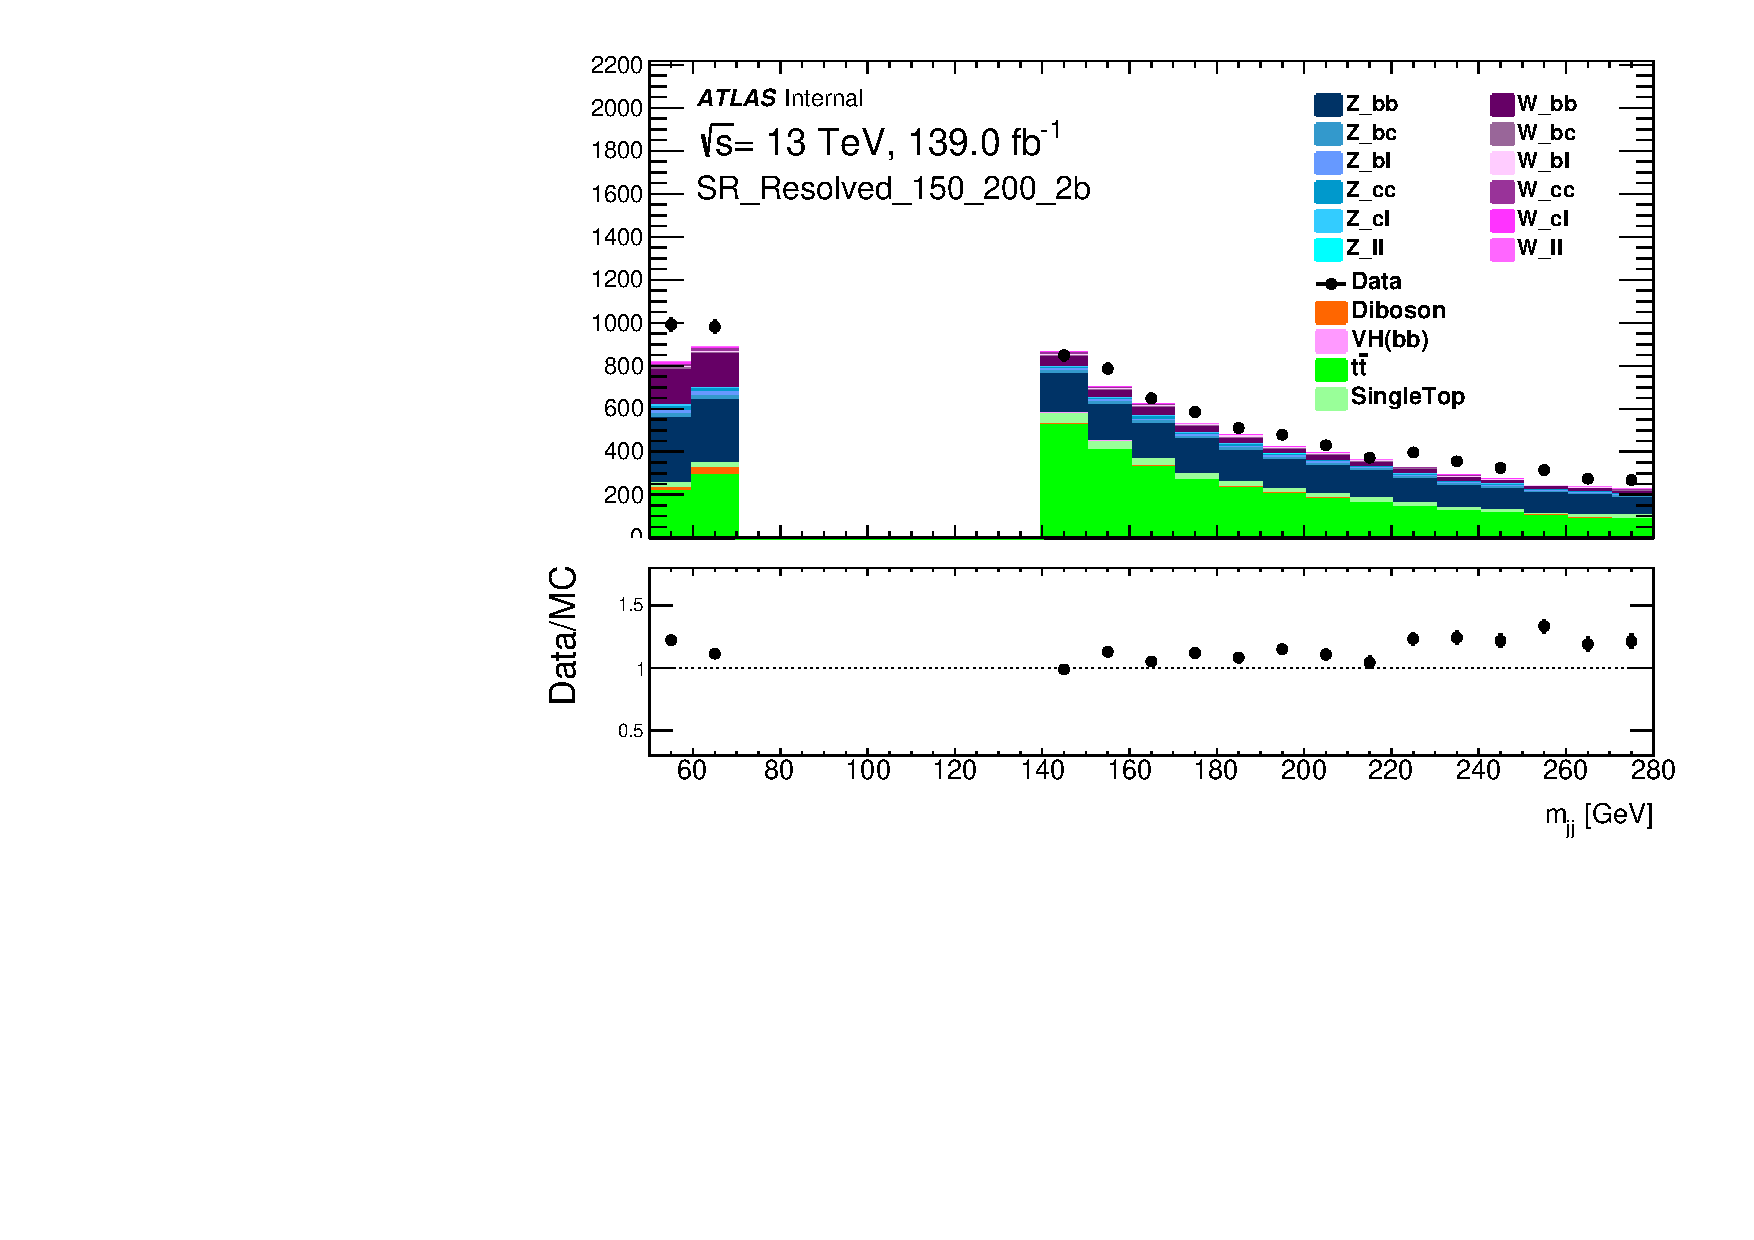
\includegraphics[width=0.46\linewidth]{chapters/c8/figures/0L/DataMC_MonoH_Nominal_SR_Resolved_150_200_2b_m_jj_10GeV.pdf}
    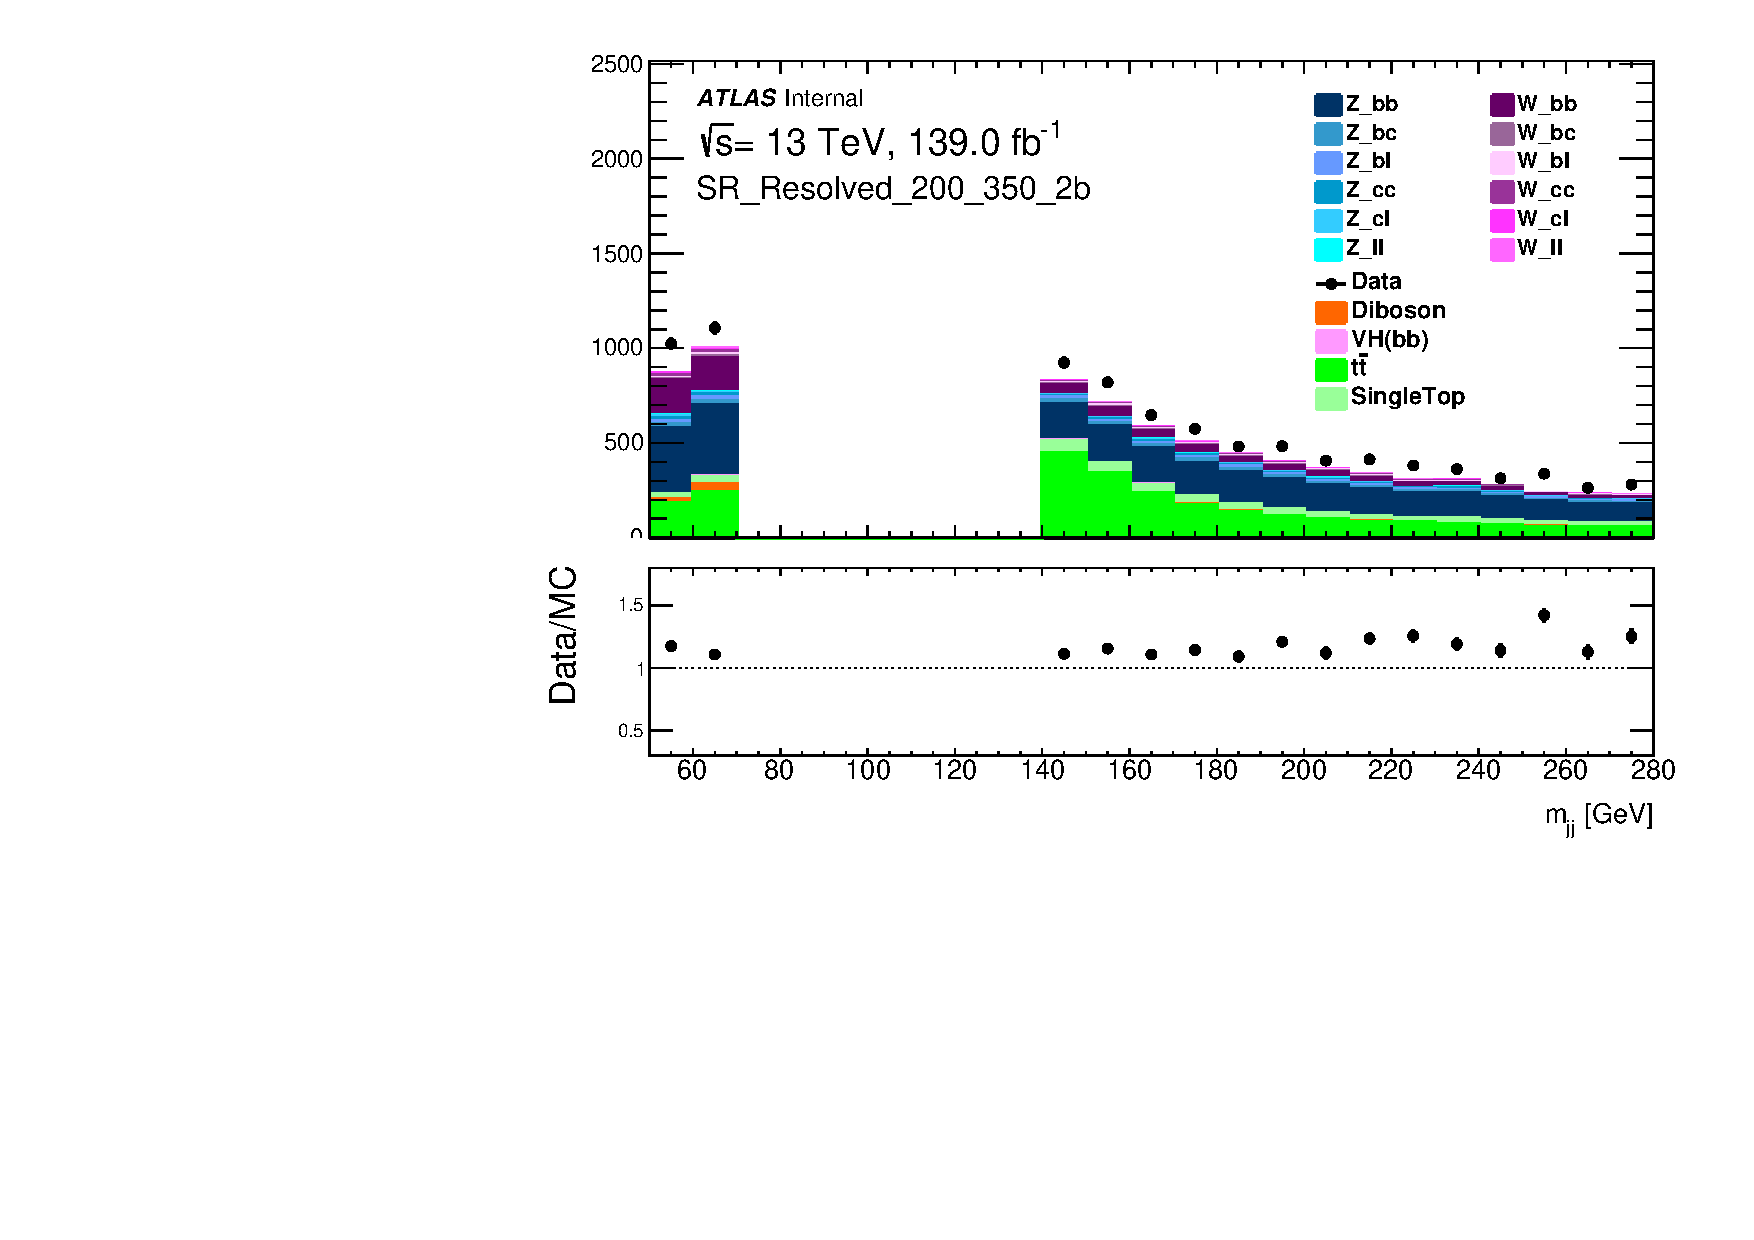
\includegraphics[width=0.46\linewidth]{chapters/c8/figures/0L/DataMC_MonoH_Nominal_SR_Resolved_200_350_2b_m_jj_10GeV.pdf}\\
    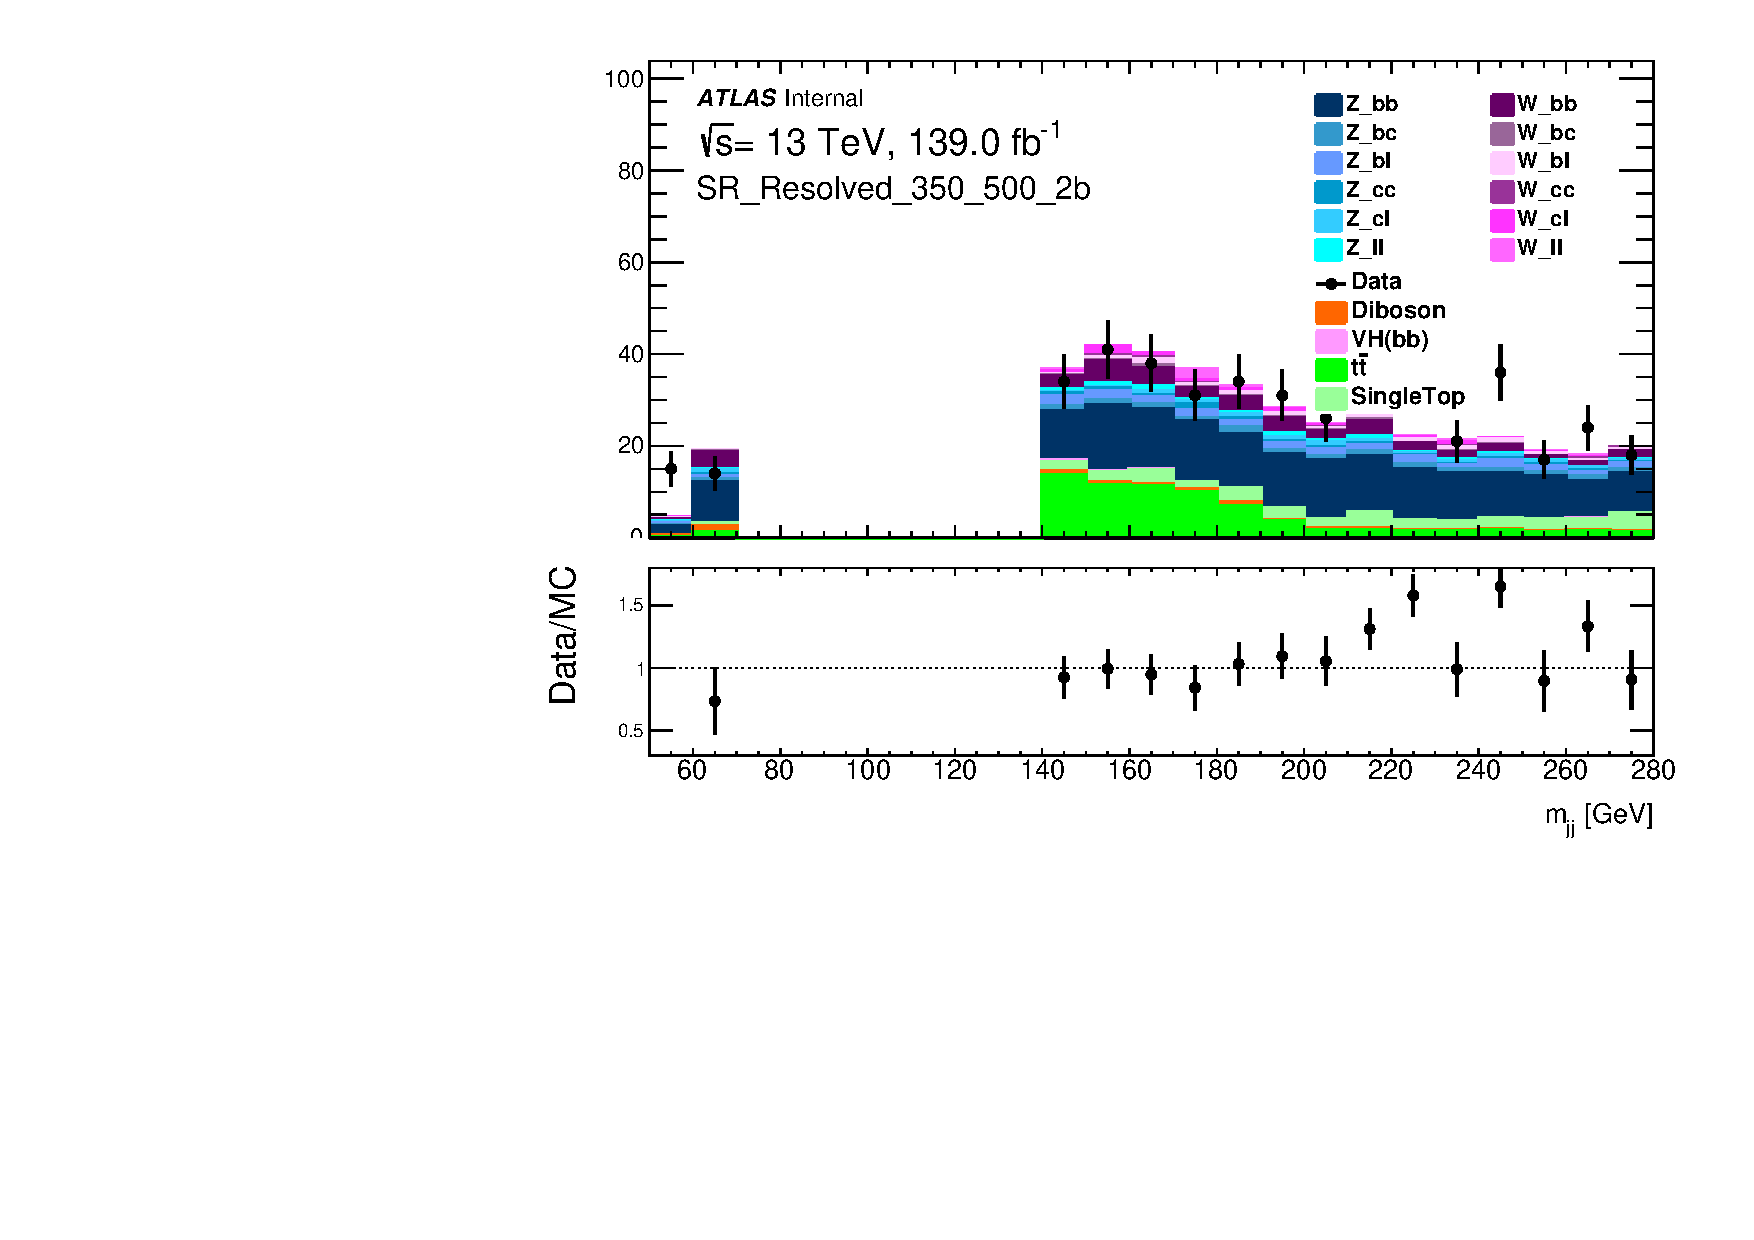
\includegraphics[width=0.46\linewidth]{chapters/c8/figures/0L/DataMC_MonoH_Nominal_SR_Resolved_350_500_2b_m_jj_10GeV.pdf}
    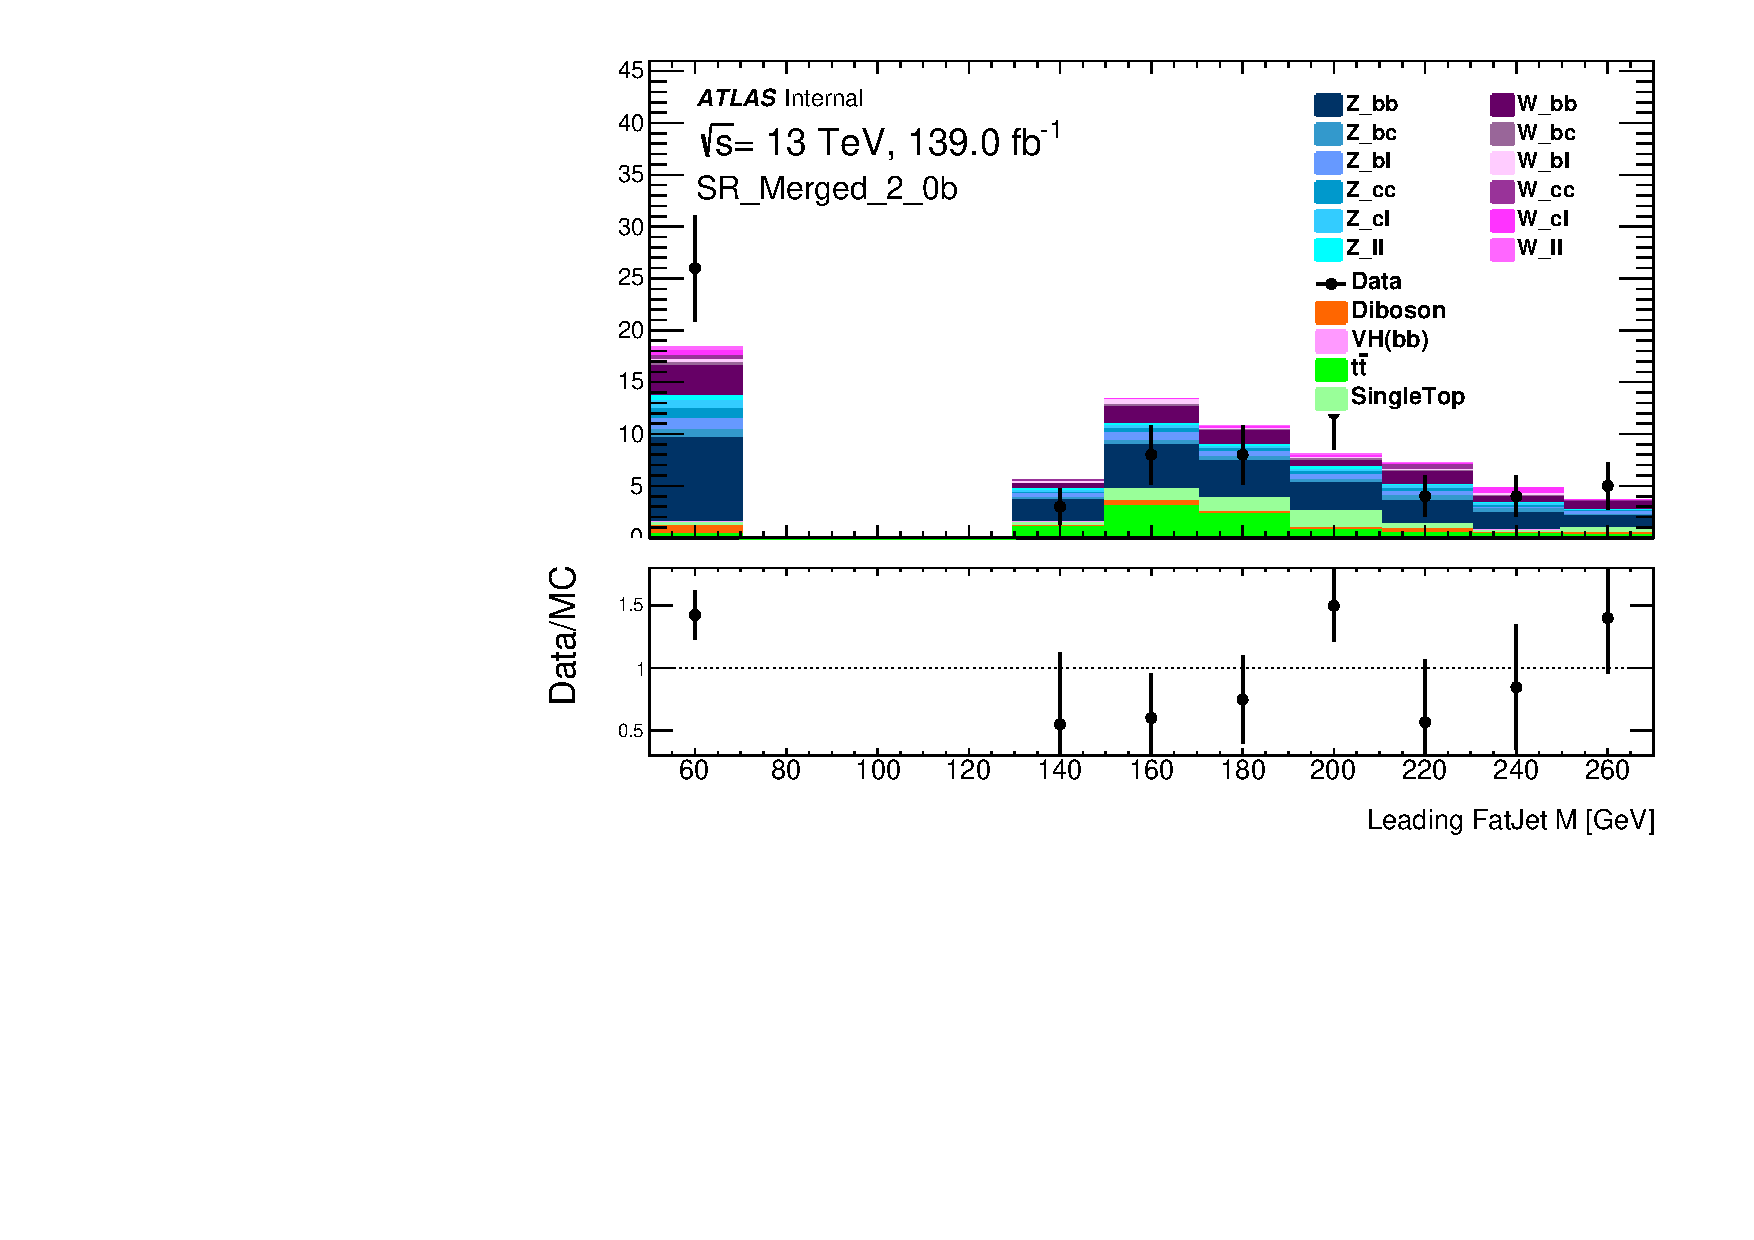
\includegraphics[width=0.46\linewidth]{chapters/c8/figures/0L/DataMC_MonoH_Nominal_SR_Merged_2_0b_fatjets_m1_20GeV.pdf}
    \caption{Higgs candidate mass spectra in the different \met~regions with 2 $b$-tagged jets in the 0-lepton channel.}
    \label{fig:data-mc-0l-mjj-2b}
\end{figure}

\begin{figure}[!htb]
    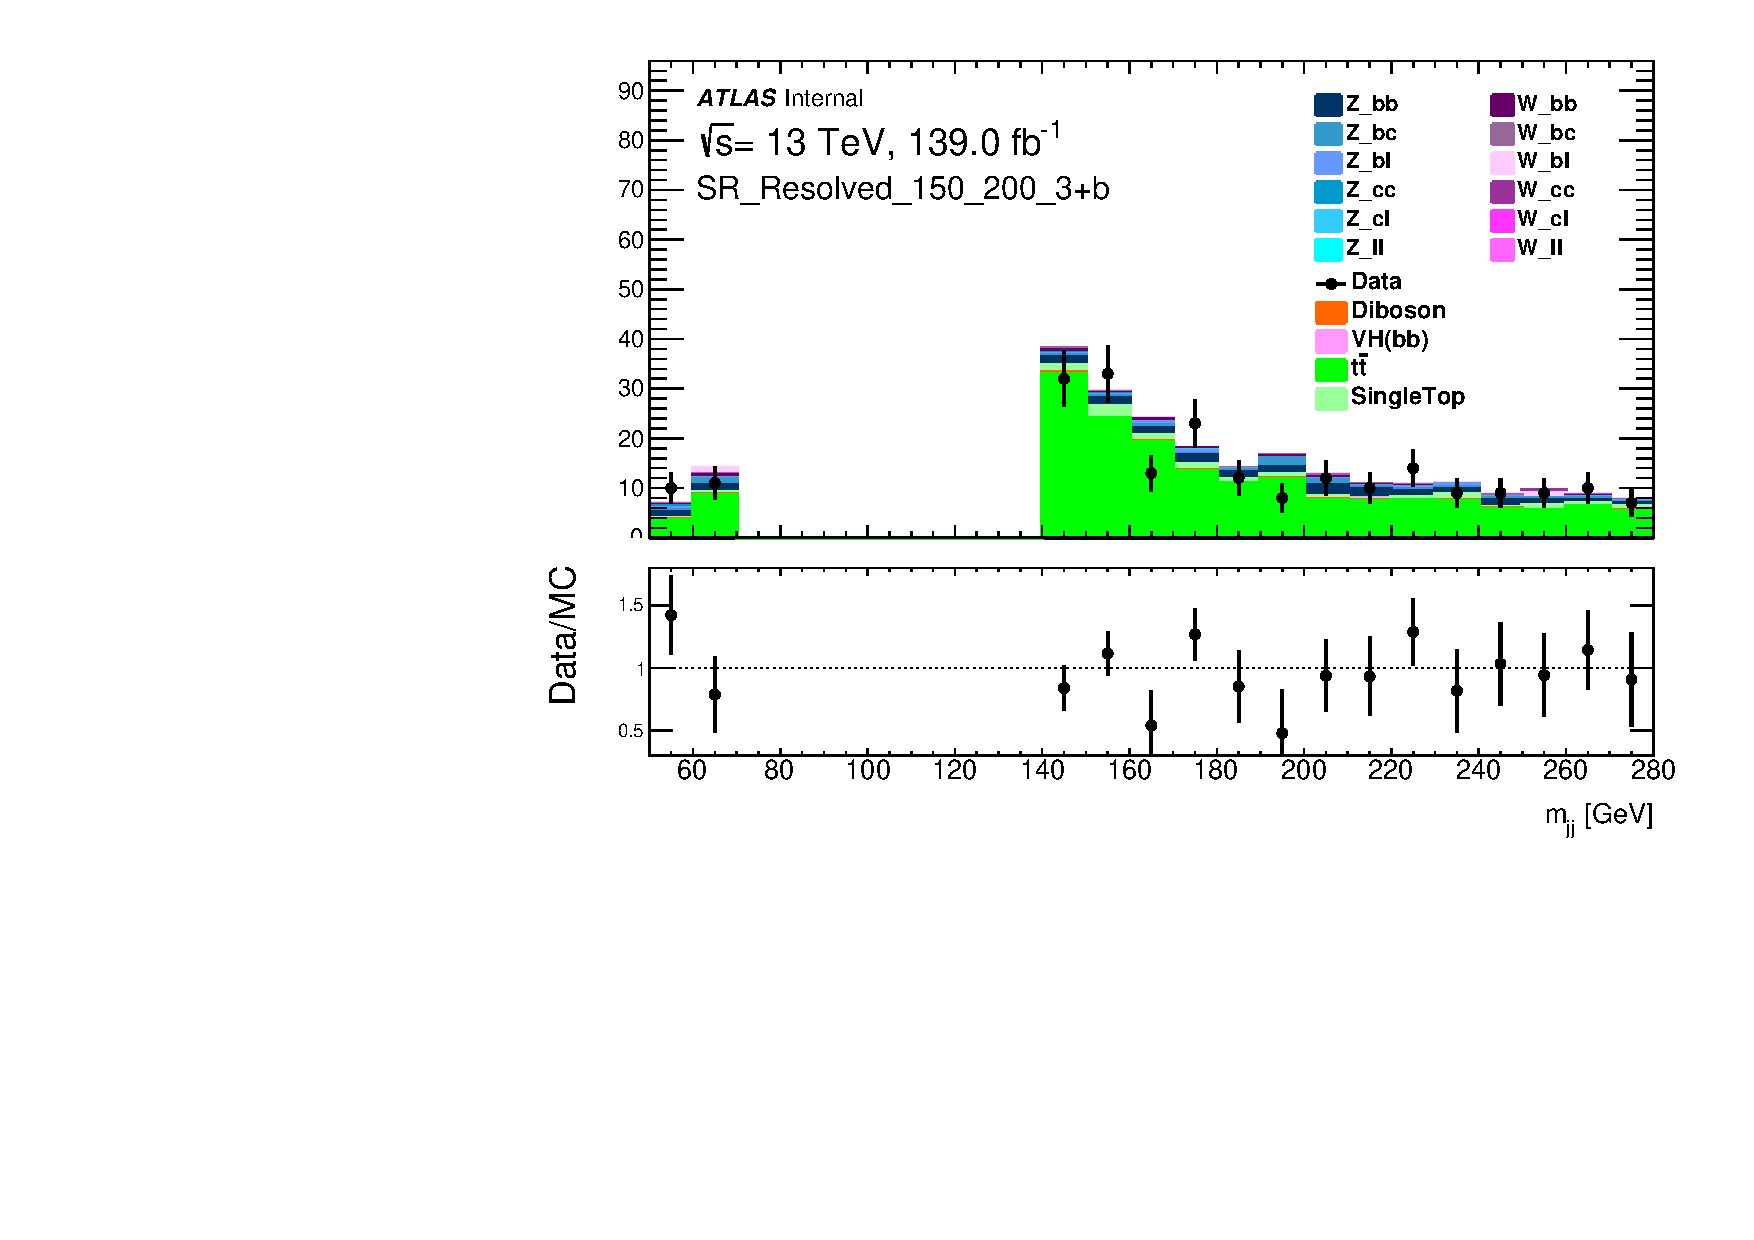
\includegraphics[width=0.46\linewidth]{chapters/c8/figures/0L/DataMC_MonoH_Nominal_SR_Resolved_150_200_3+b_m_jj_10GeV.pdf}
    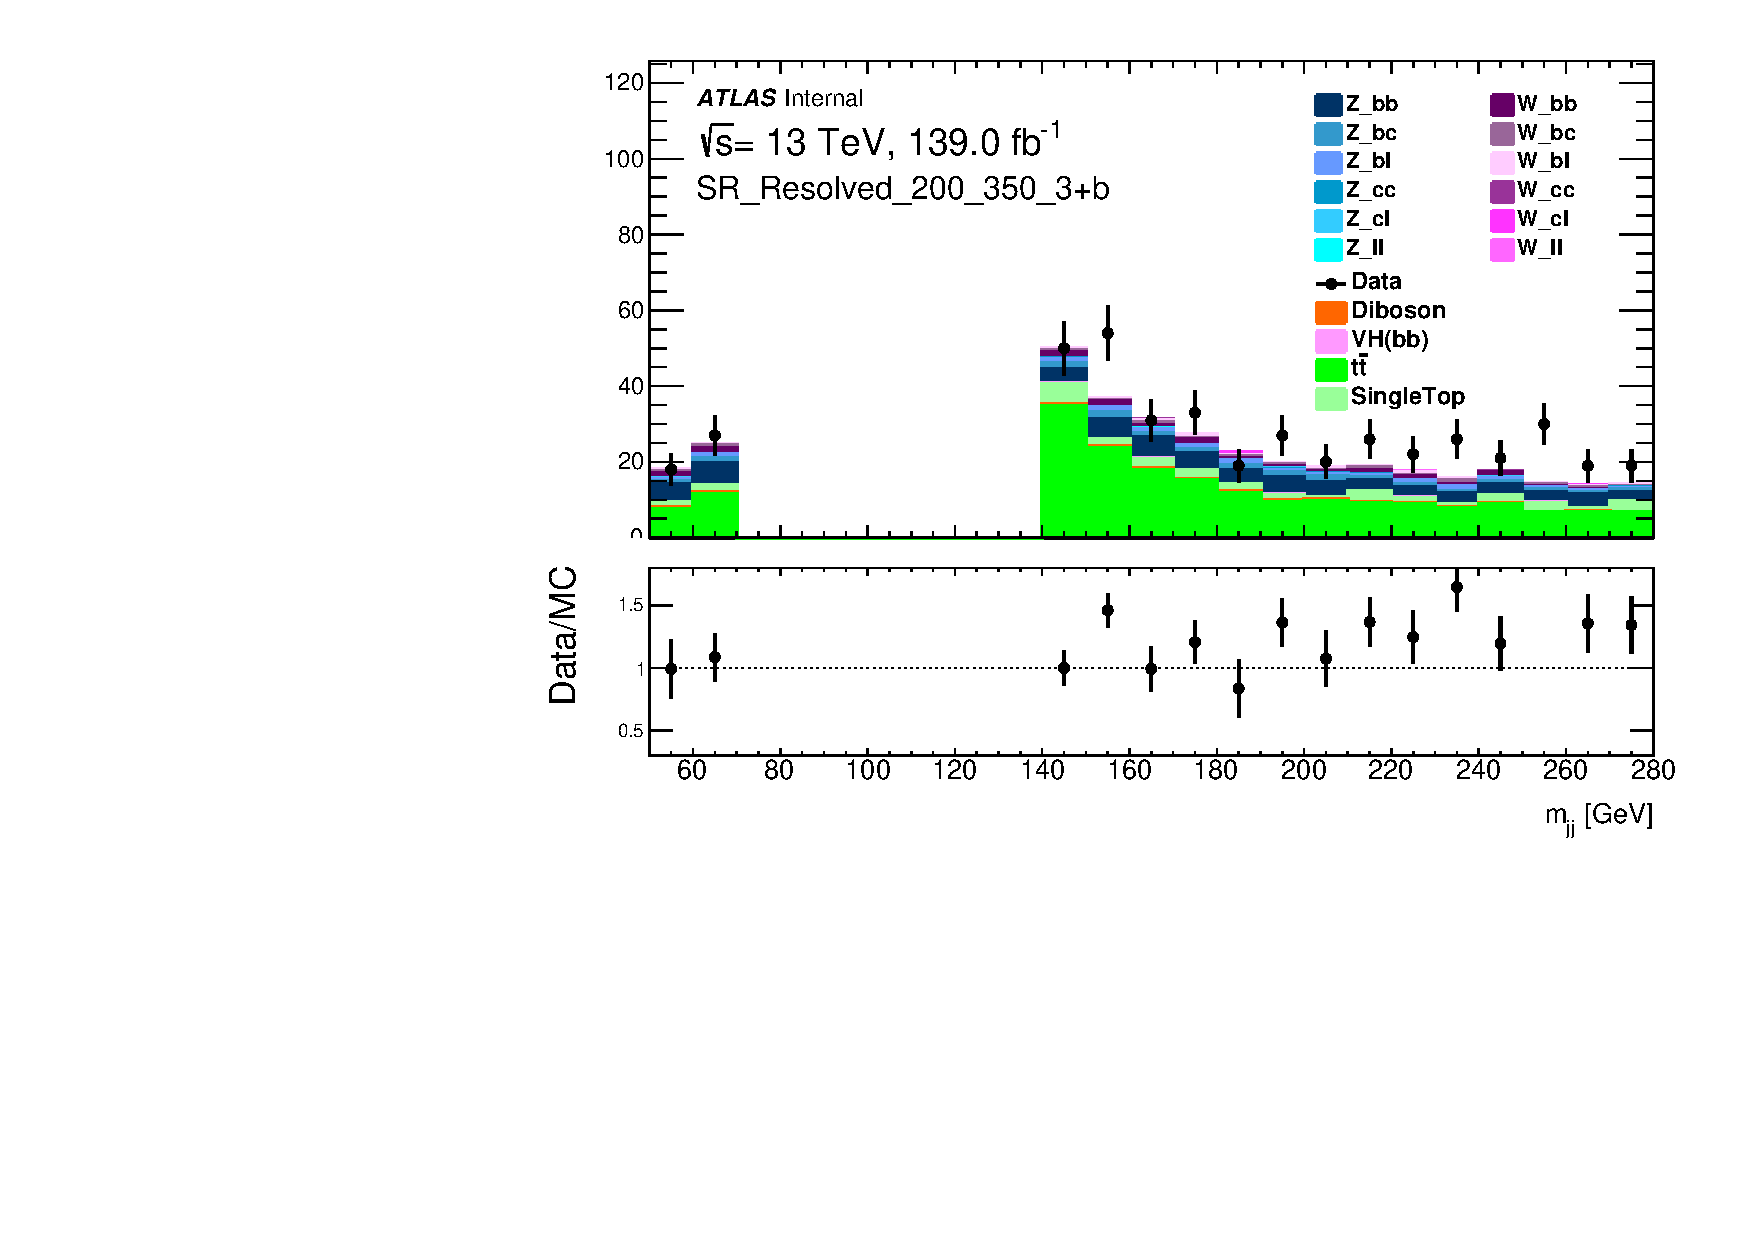
\includegraphics[width=0.46\linewidth]{chapters/c8/figures/0L/DataMC_MonoH_Nominal_SR_Resolved_200_350_3+b_m_jj_10GeV.pdf}\\
    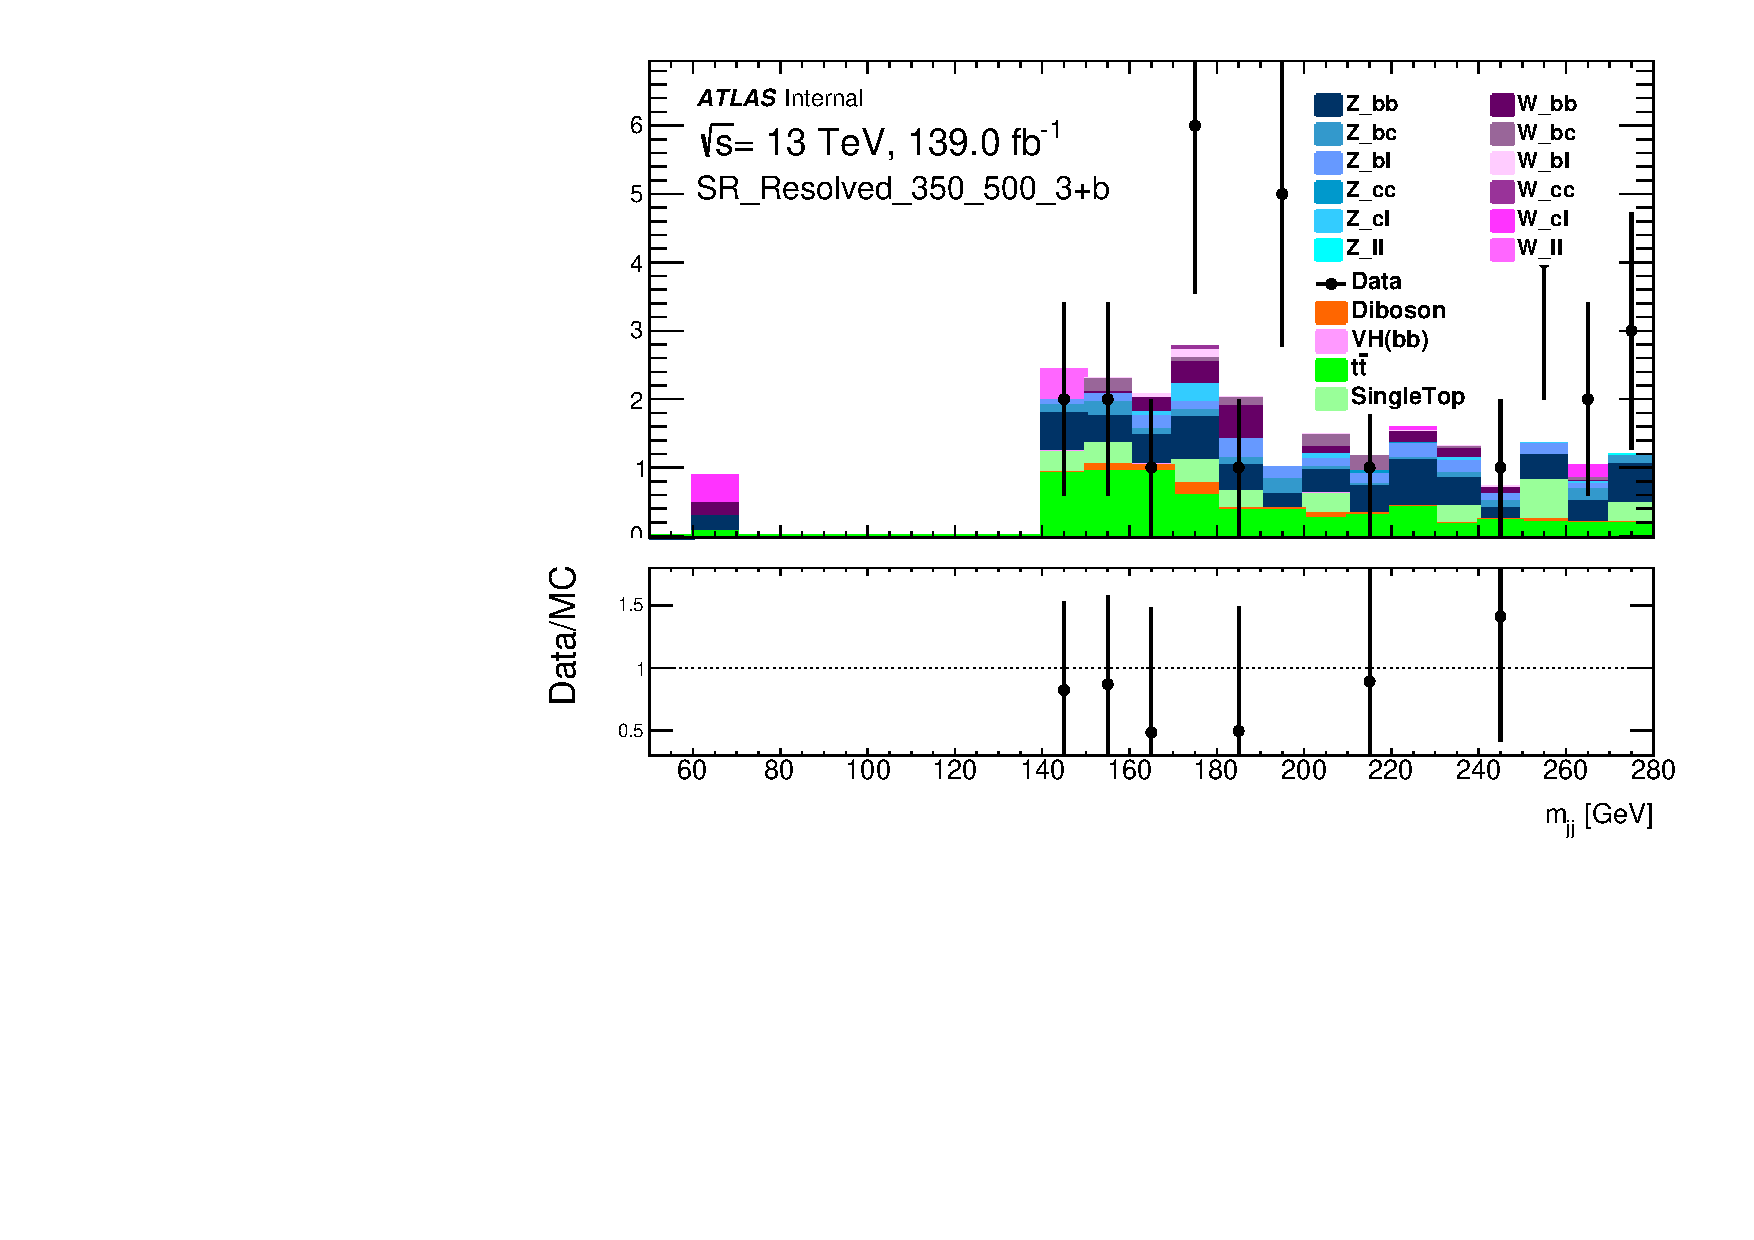
\includegraphics[width=0.46\linewidth]{chapters/c8/figures/0L/DataMC_MonoH_Nominal_SR_Resolved_350_500_3+b_m_jj_10GeV.pdf}
    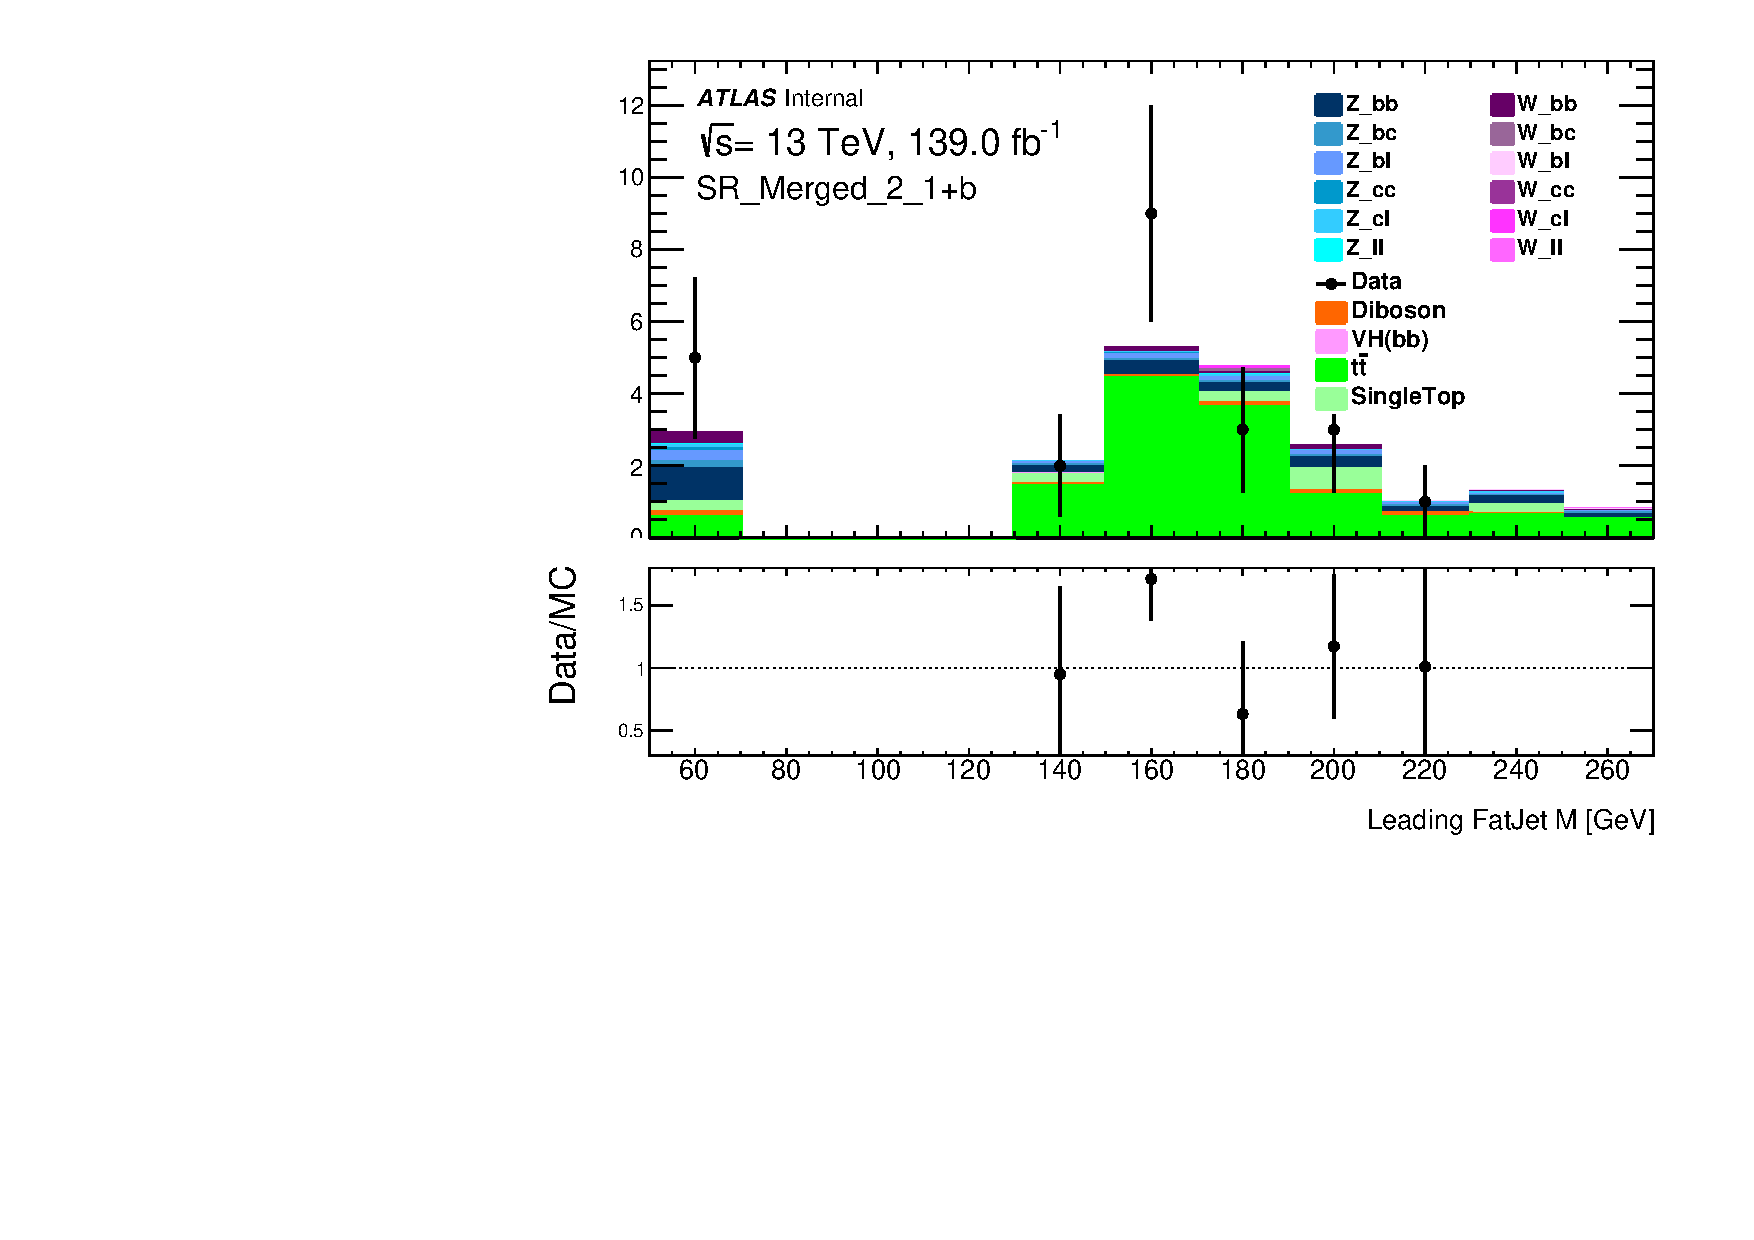
\includegraphics[width=0.46\linewidth]{chapters/c8/figures/0L/DataMC_MonoH_Nominal_SR_Merged_2_1+b_fatjets_m1_20GeV.pdf}
    \caption{Higgs candidate mass spectra in the different \met~regions with at least 3 $b$-tagged jets in the 0-lepton channel.}
    \label{fig:data-mc-0l-mjj-3+b}
\end{figure}

\begin{figure}[!htb]
    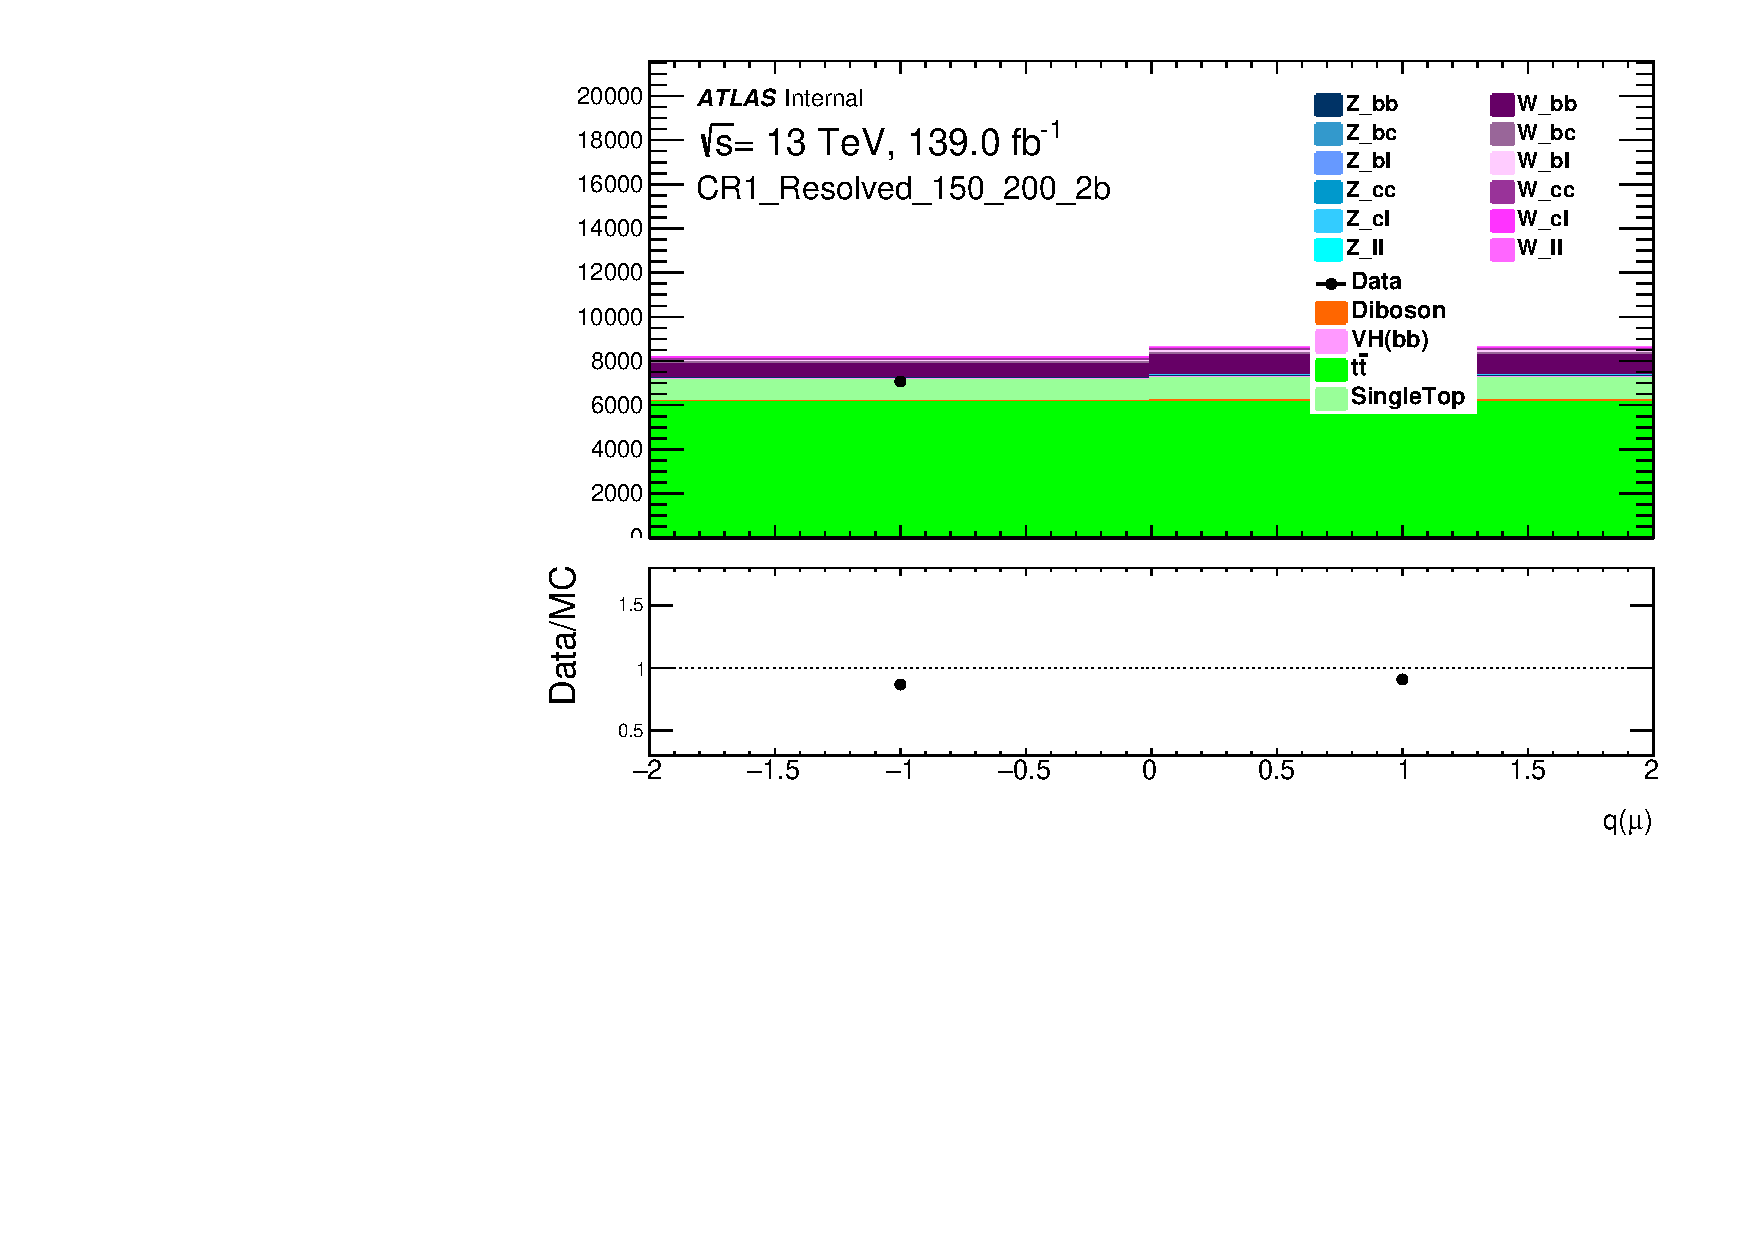
\includegraphics[width=0.46\linewidth]{chapters/c8/figures/1L/DataMC_MonoH_Nominal_CR1_Resolved_150_200_2b_mu_charge.pdf}
    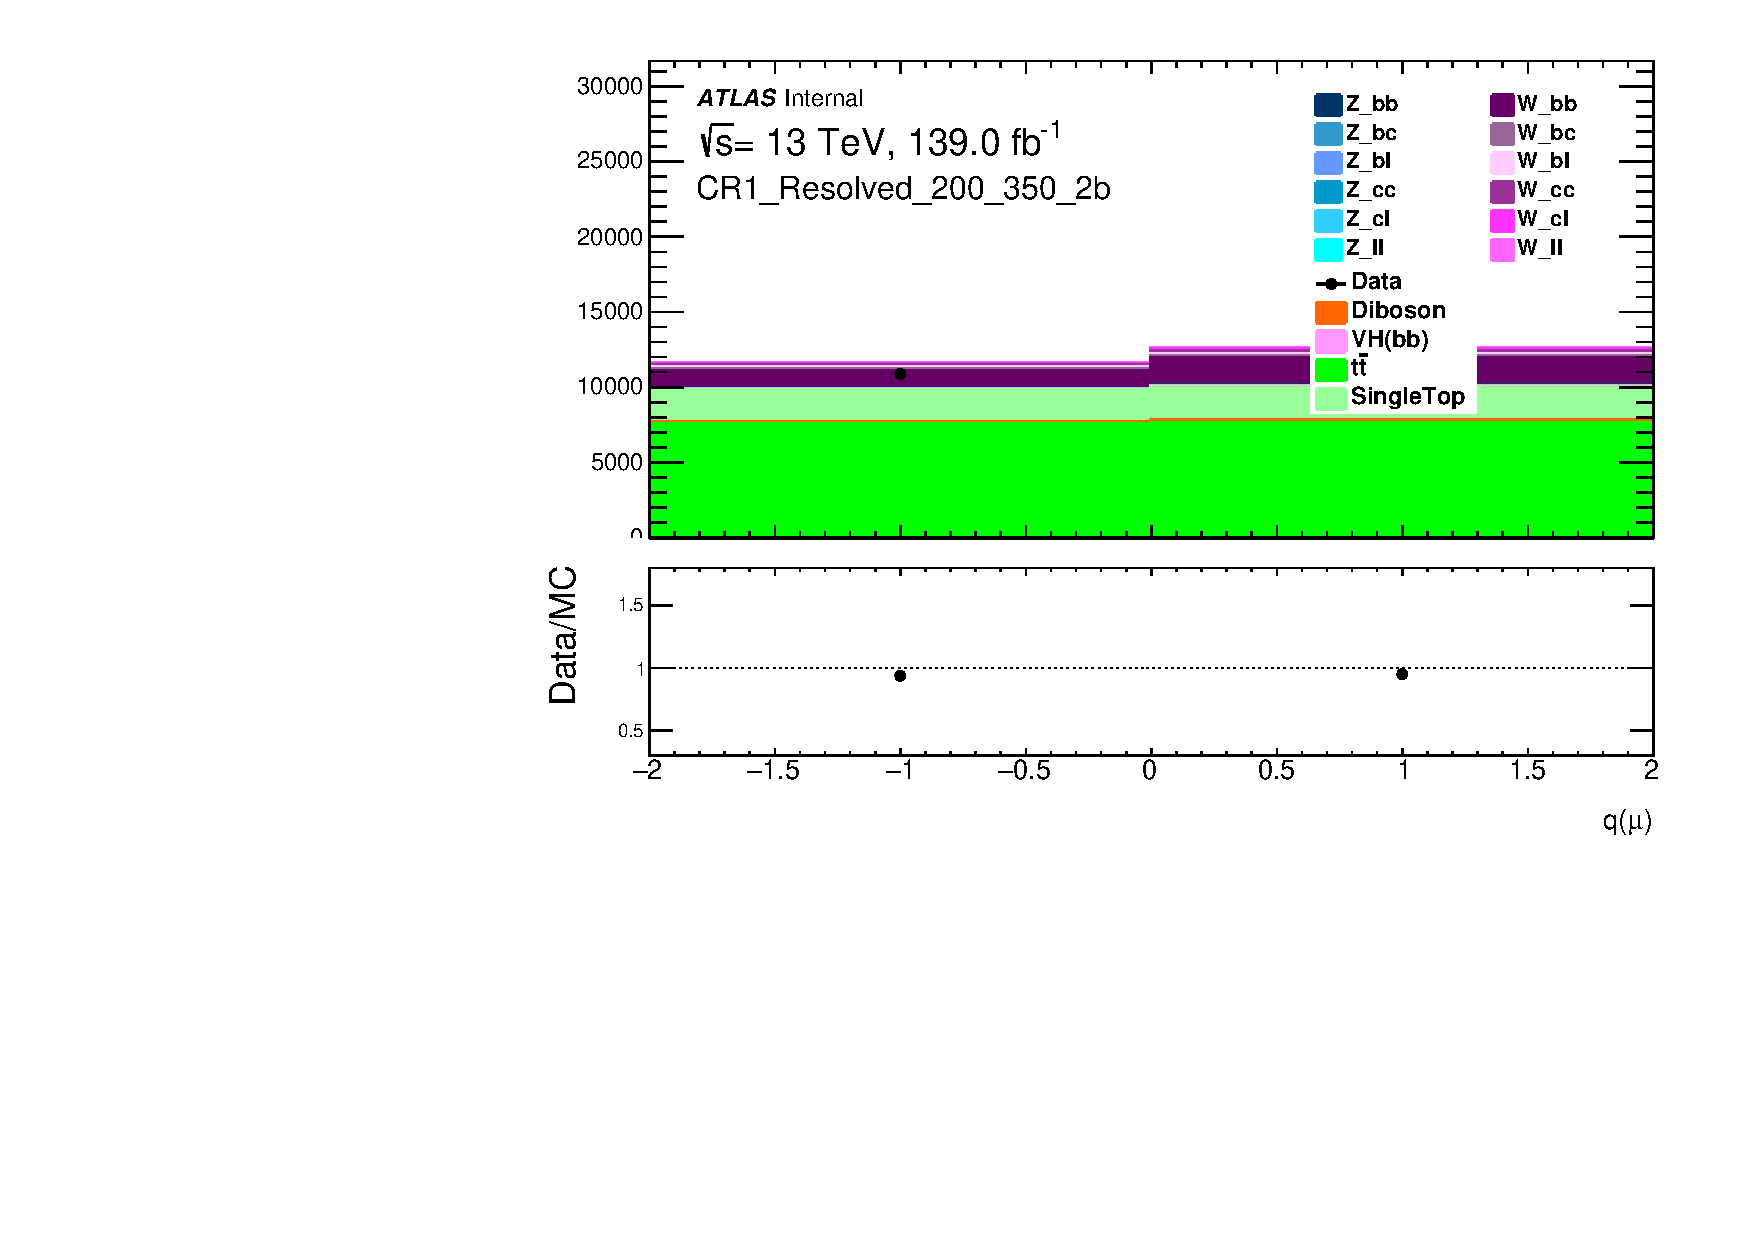
\includegraphics[width=0.46\linewidth]{chapters/c8/figures/1L/DataMC_MonoH_Nominal_CR1_Resolved_200_350_2b_mu_charge.pdf}\\
    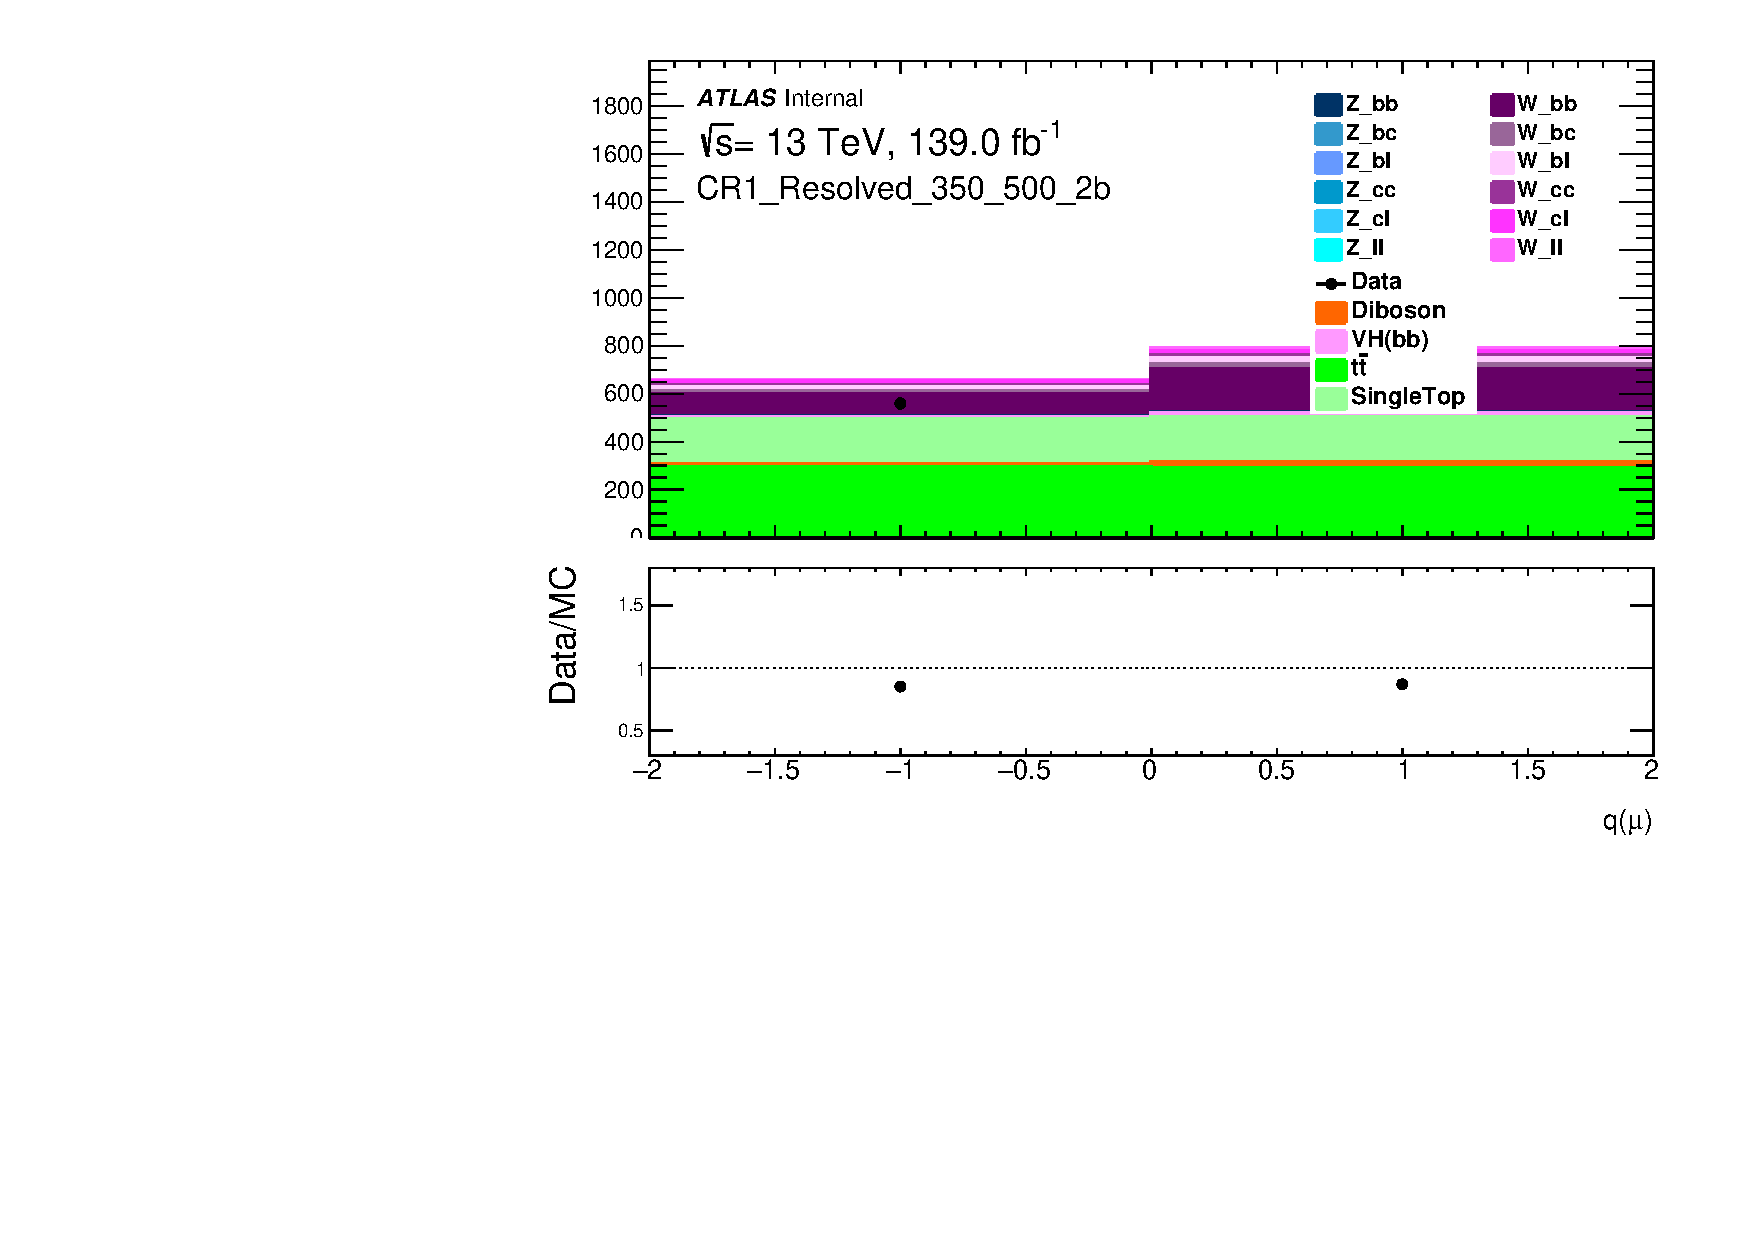
\includegraphics[width=0.46\linewidth]{chapters/c8/figures/1L/DataMC_MonoH_Nominal_CR1_Resolved_350_500_2b_mu_charge.pdf}
    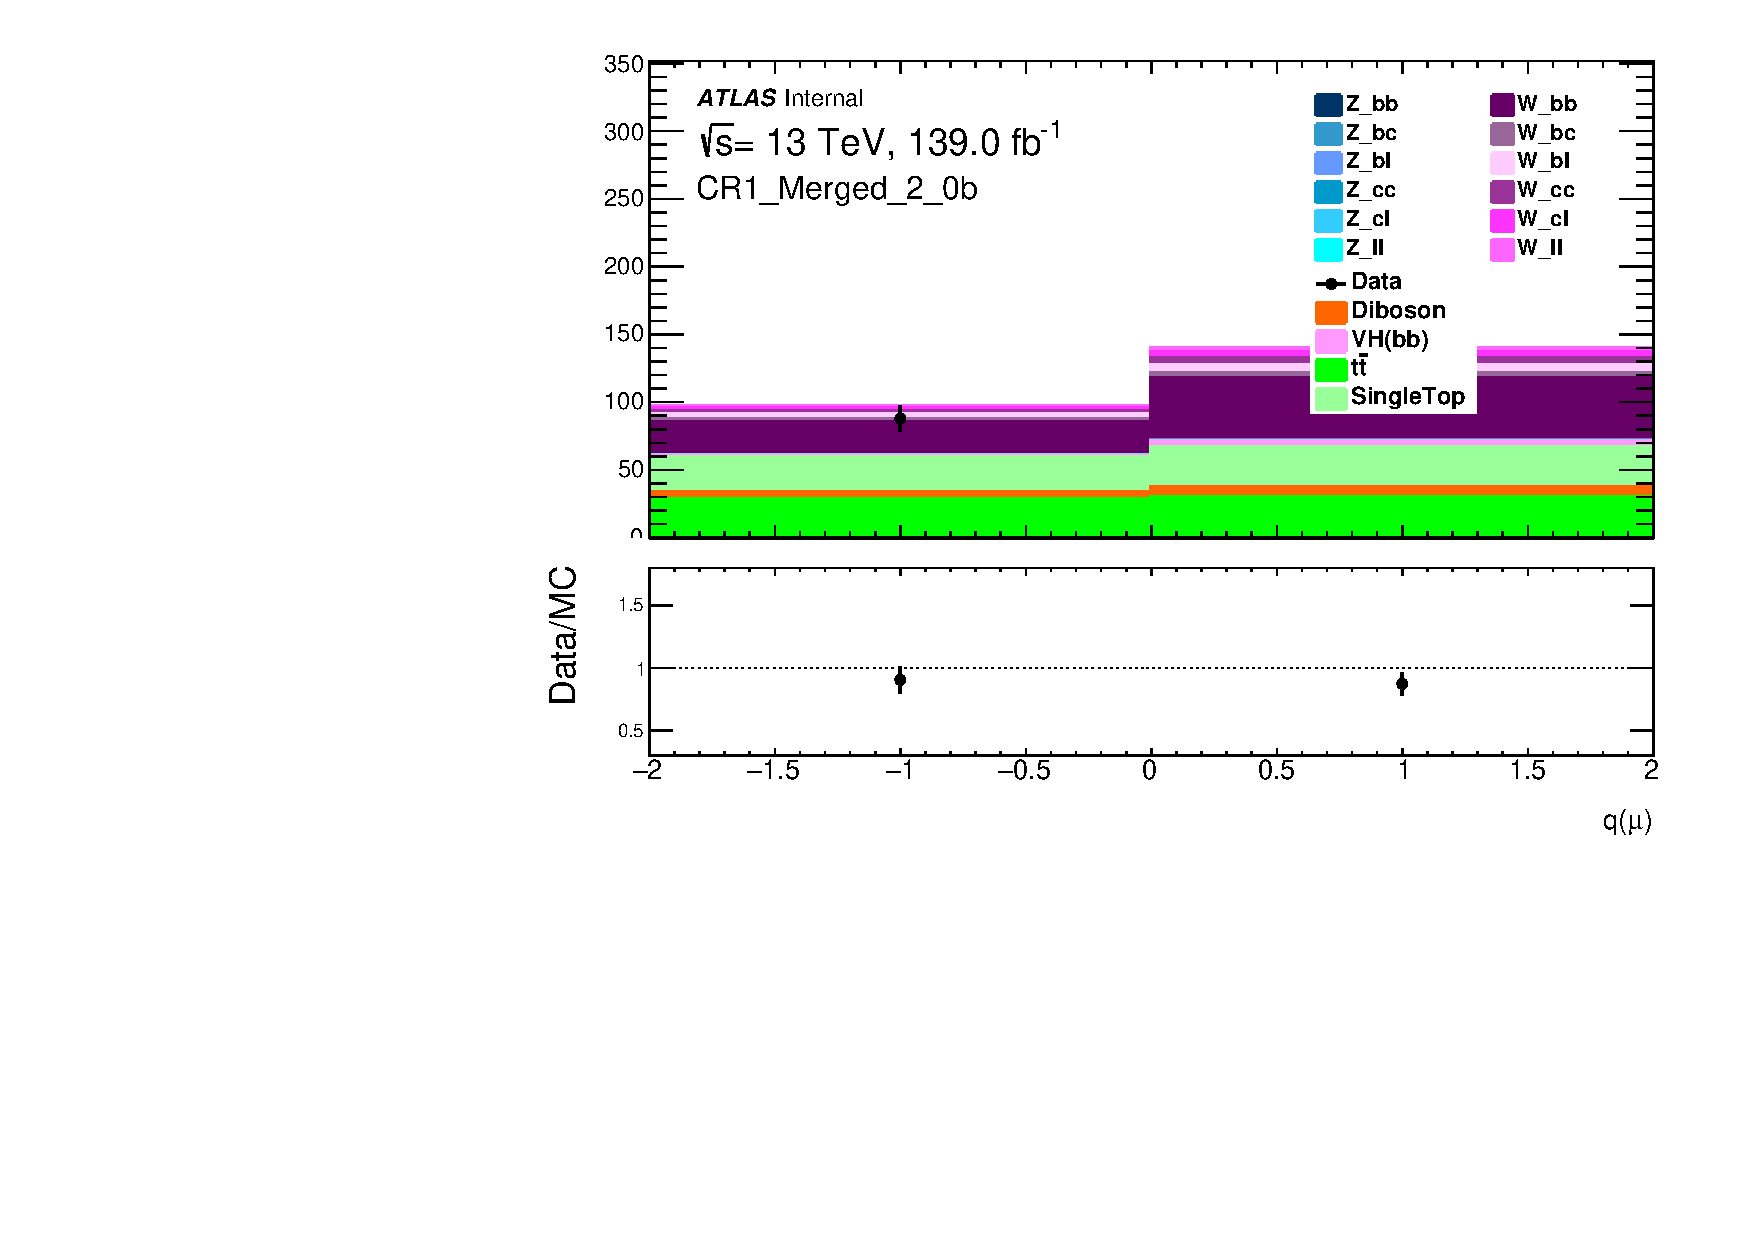
\includegraphics[width=0.46\linewidth]{chapters/c8/figures/1L/DataMC_MonoH_Nominal_CR1_Merged_2_0b_mu_charge.pdf}
    \caption{Muon charge distribution in the different \met~regions with 2 $b$-tagged jets in the 1-lepton channel.}
    \label{fig:data-mc-1l-mu-charge-2b}
\end{figure}

\begin{figure}[!htb]
    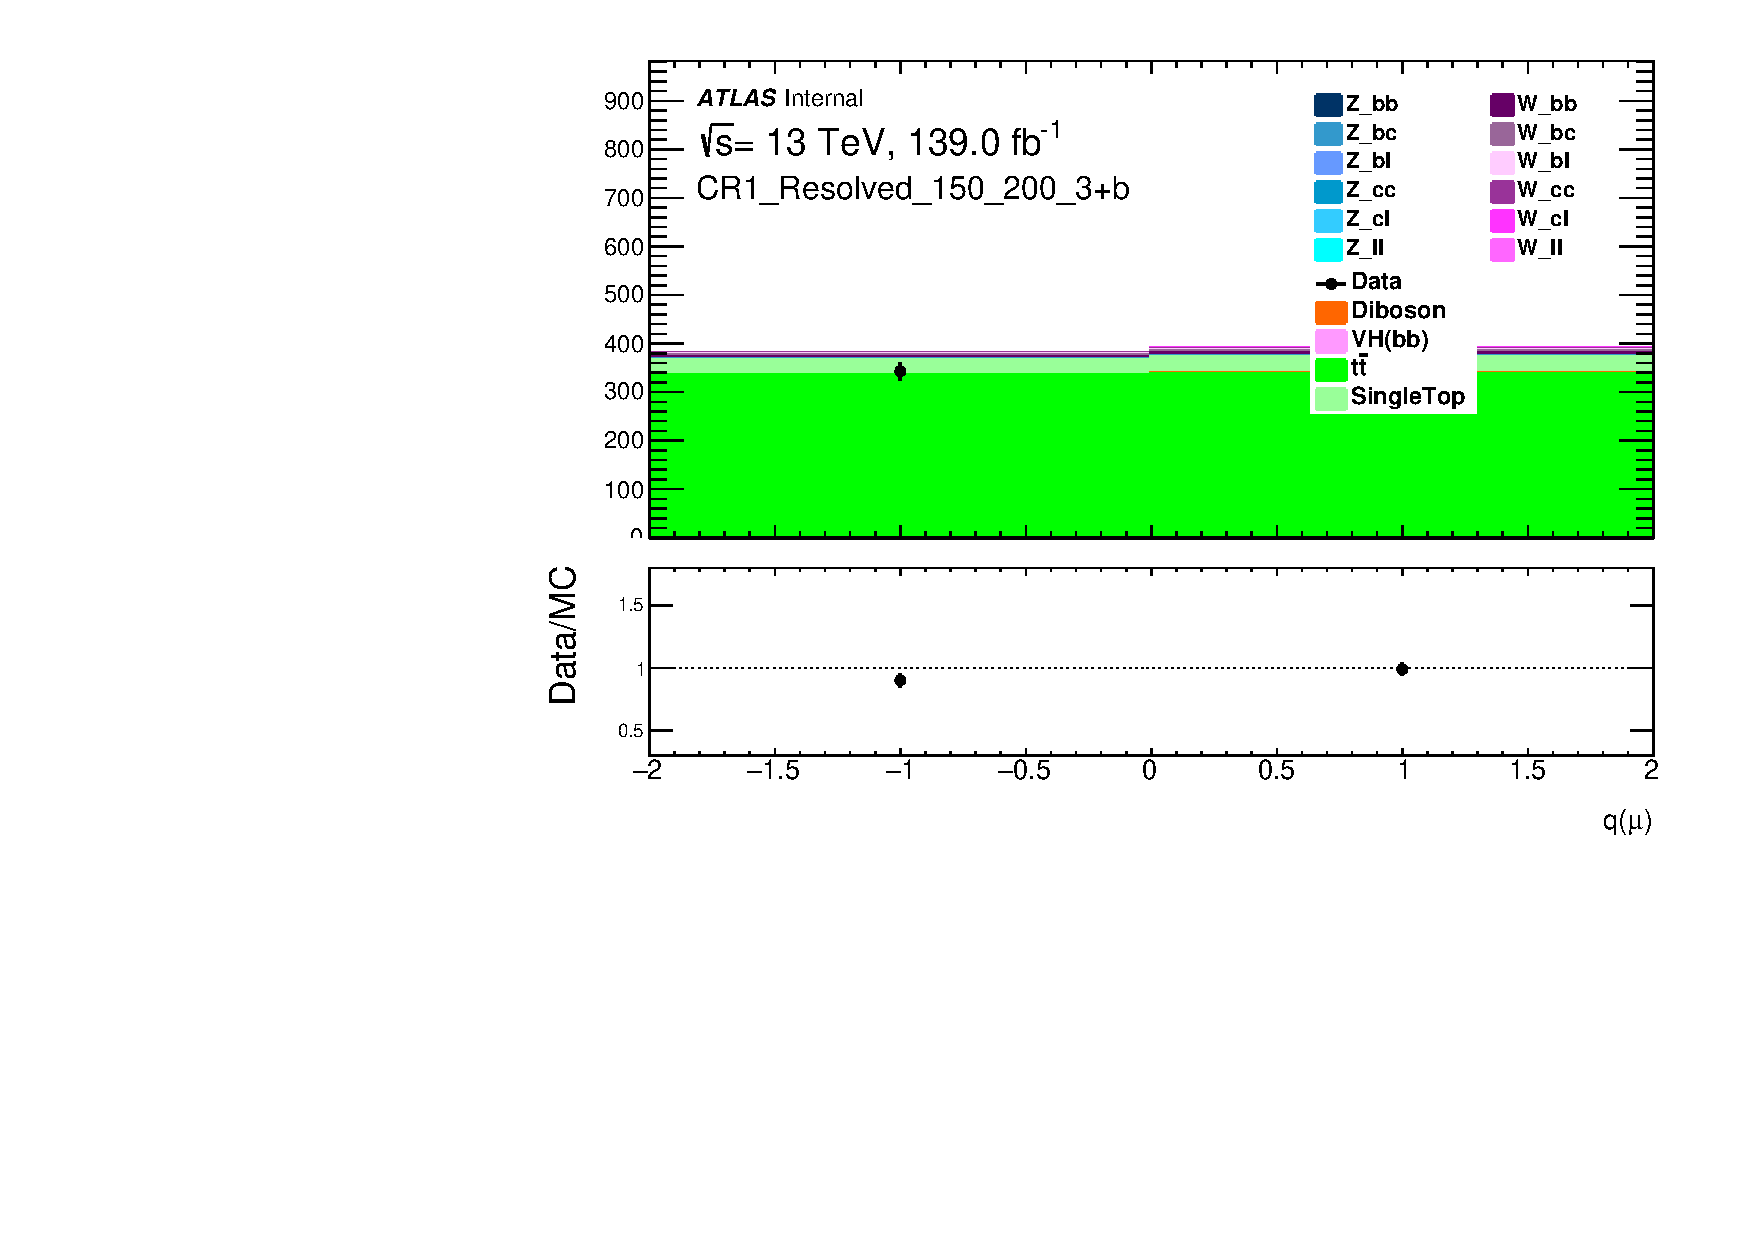
\includegraphics[width=0.46\linewidth]{chapters/c8/figures/1L/DataMC_MonoH_Nominal_CR1_Resolved_150_200_3+b_mu_charge.pdf}
    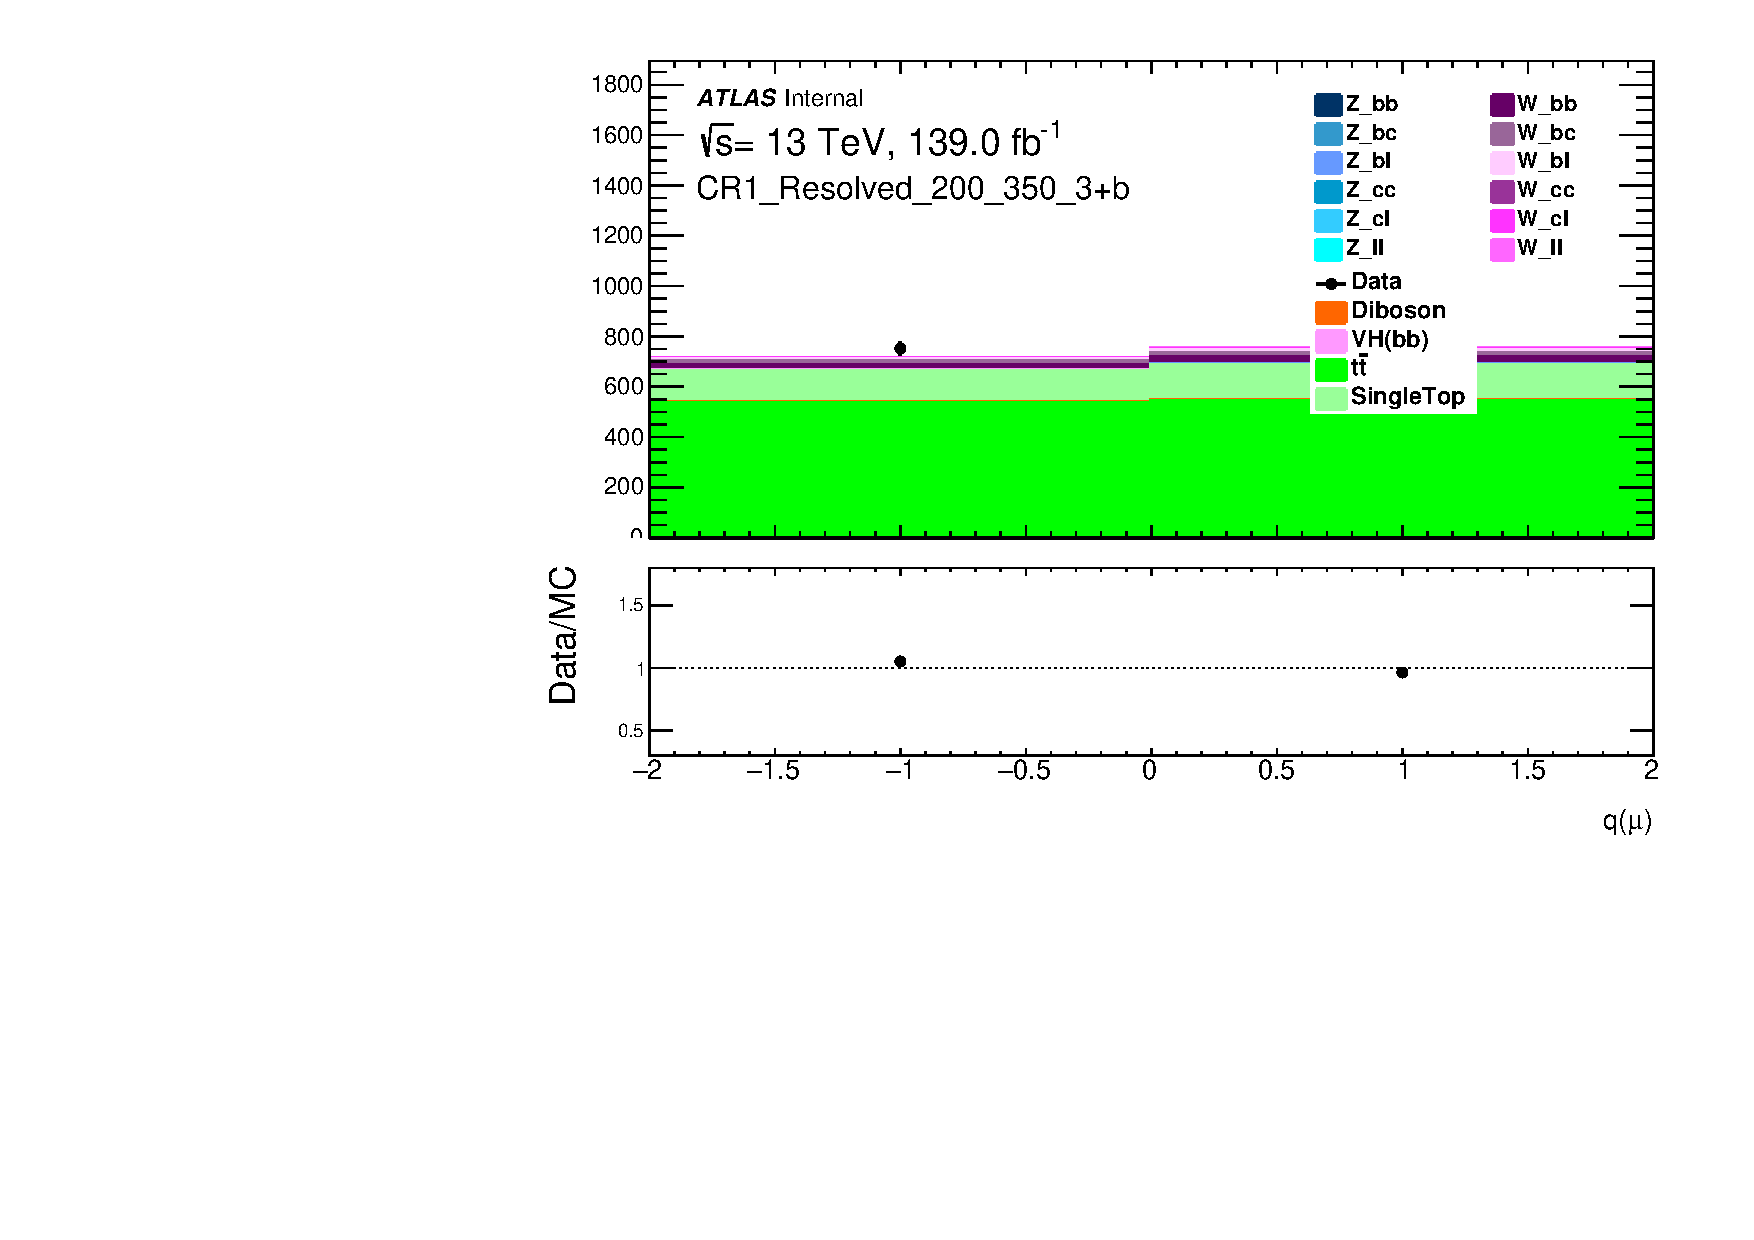
\includegraphics[width=0.46\linewidth]{chapters/c8/figures/1L/DataMC_MonoH_Nominal_CR1_Resolved_200_350_3+b_mu_charge.pdf}\\
    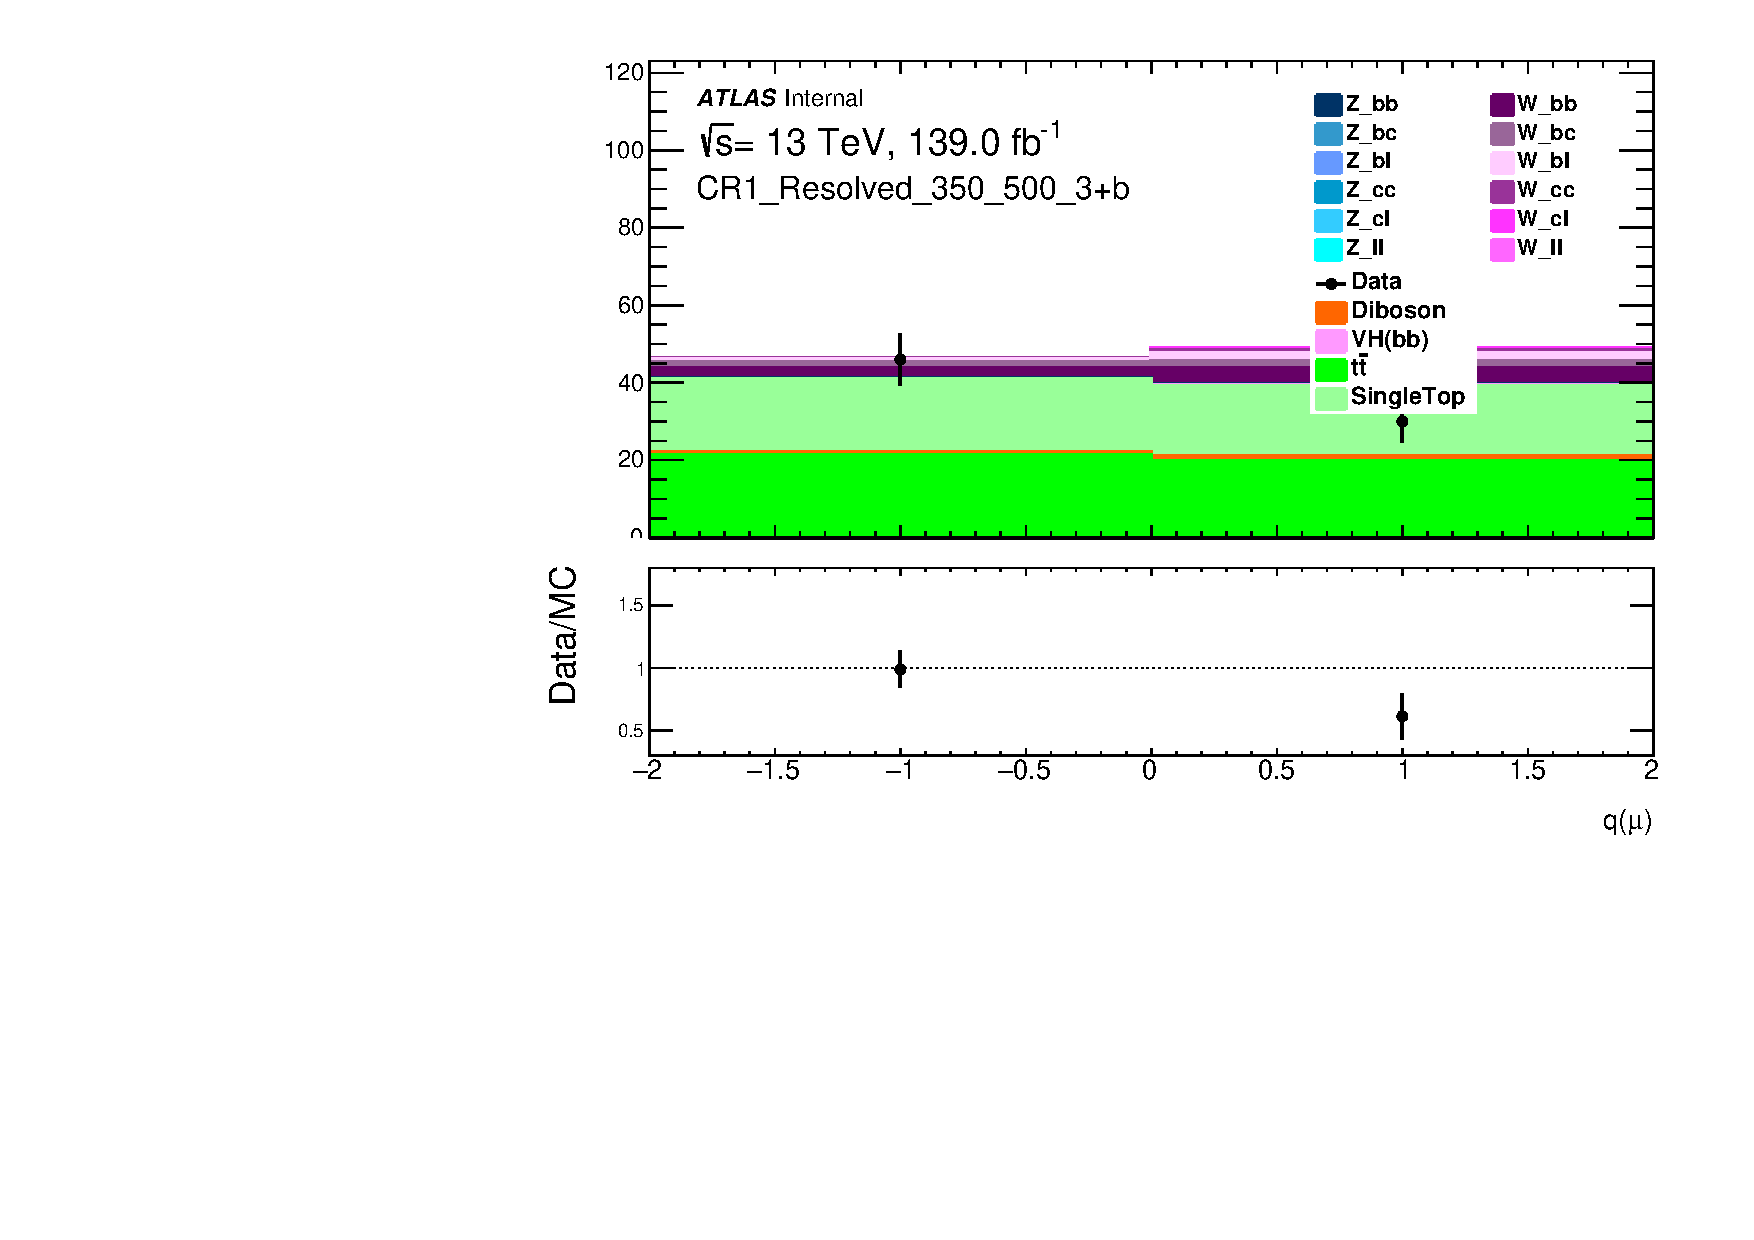
\includegraphics[width=0.46\linewidth]{chapters/c8/figures/1L/DataMC_MonoH_Nominal_CR1_Resolved_350_500_3+b_mu_charge.pdf}
    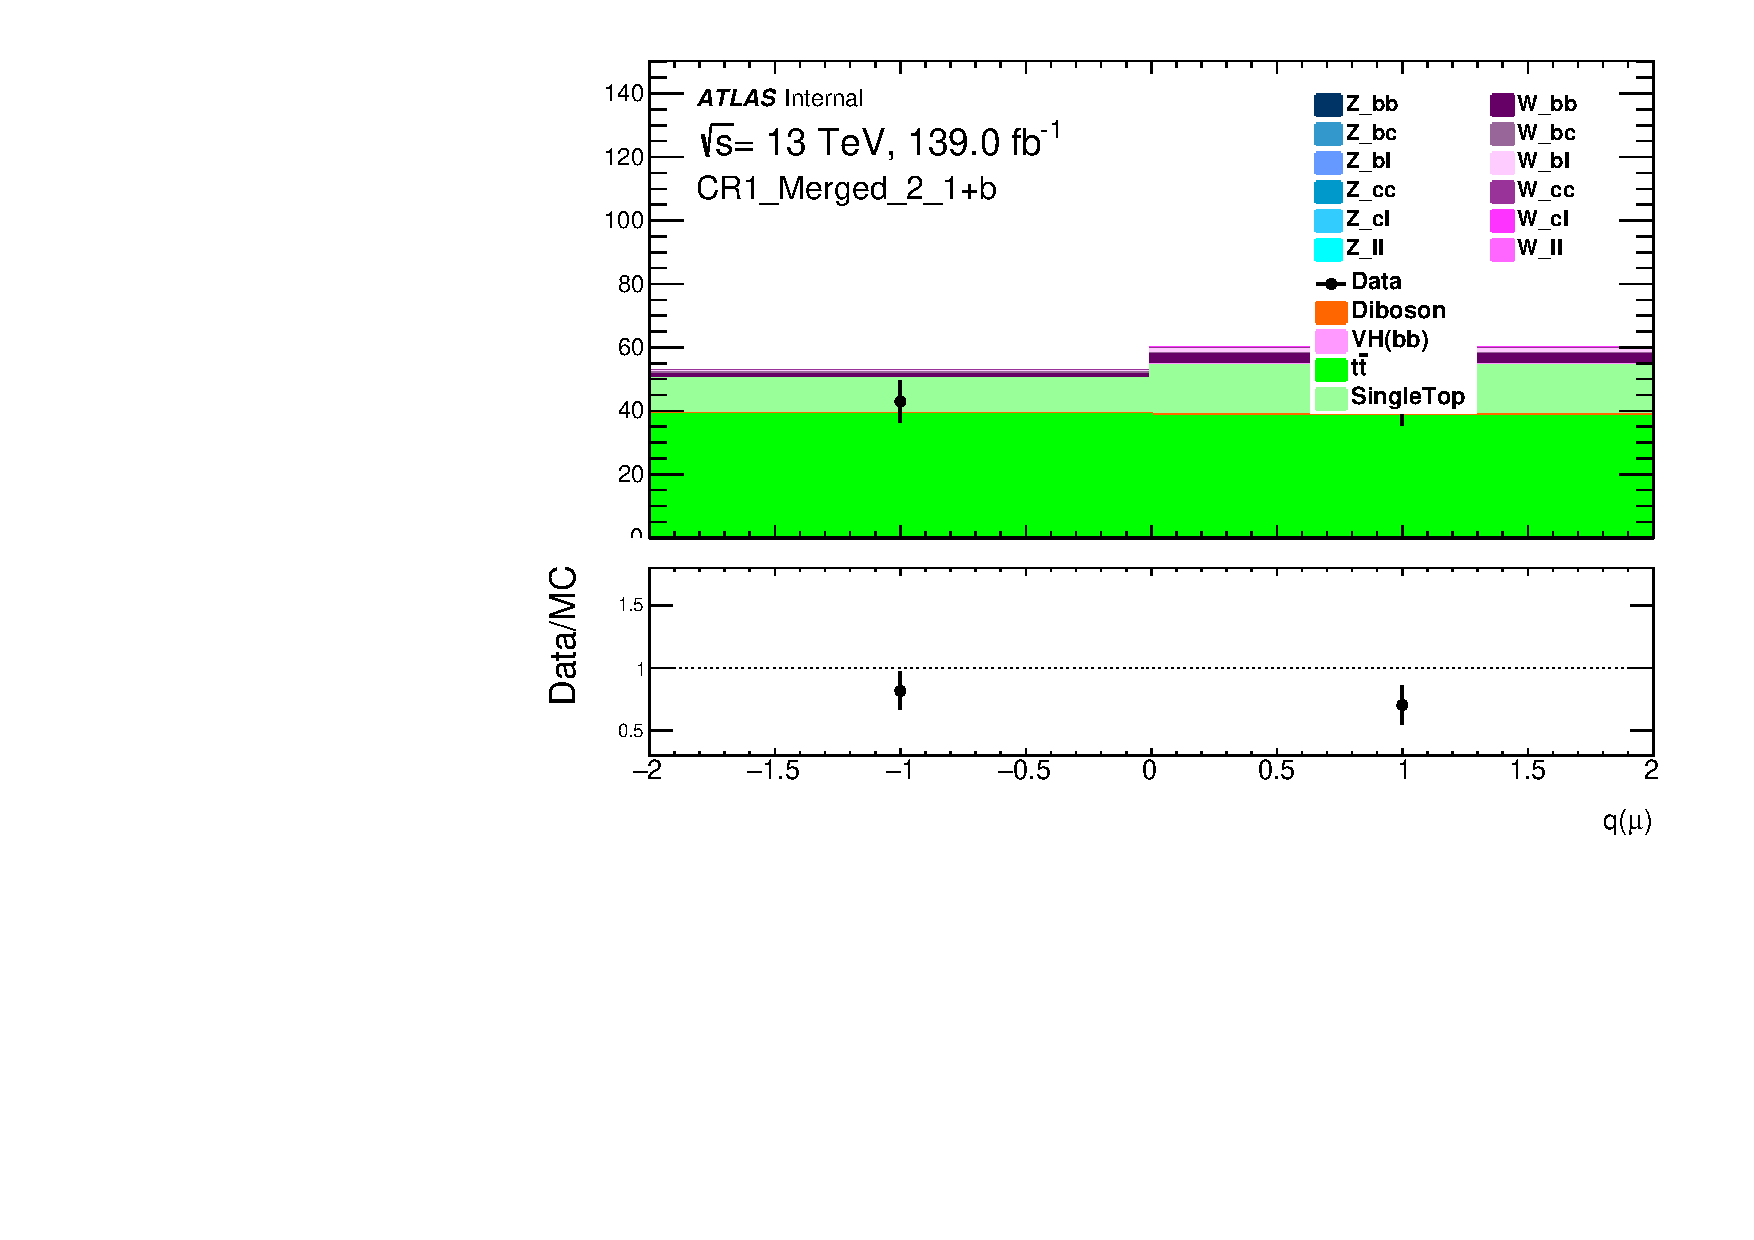
\includegraphics[width=0.46\linewidth]{chapters/c8/figures/1L/DataMC_MonoH_Nominal_CR1_Merged_2_1+b_mu_charge.pdf}
    \caption{Muon charge distribution in the different \met~regions with least 3 $b$-tagged jets in the 1-lepton channel.}
    \label{fig:data-mc-1l-mu-charge-3+b}
\end{figure}

\begin{figure}[!htb]
    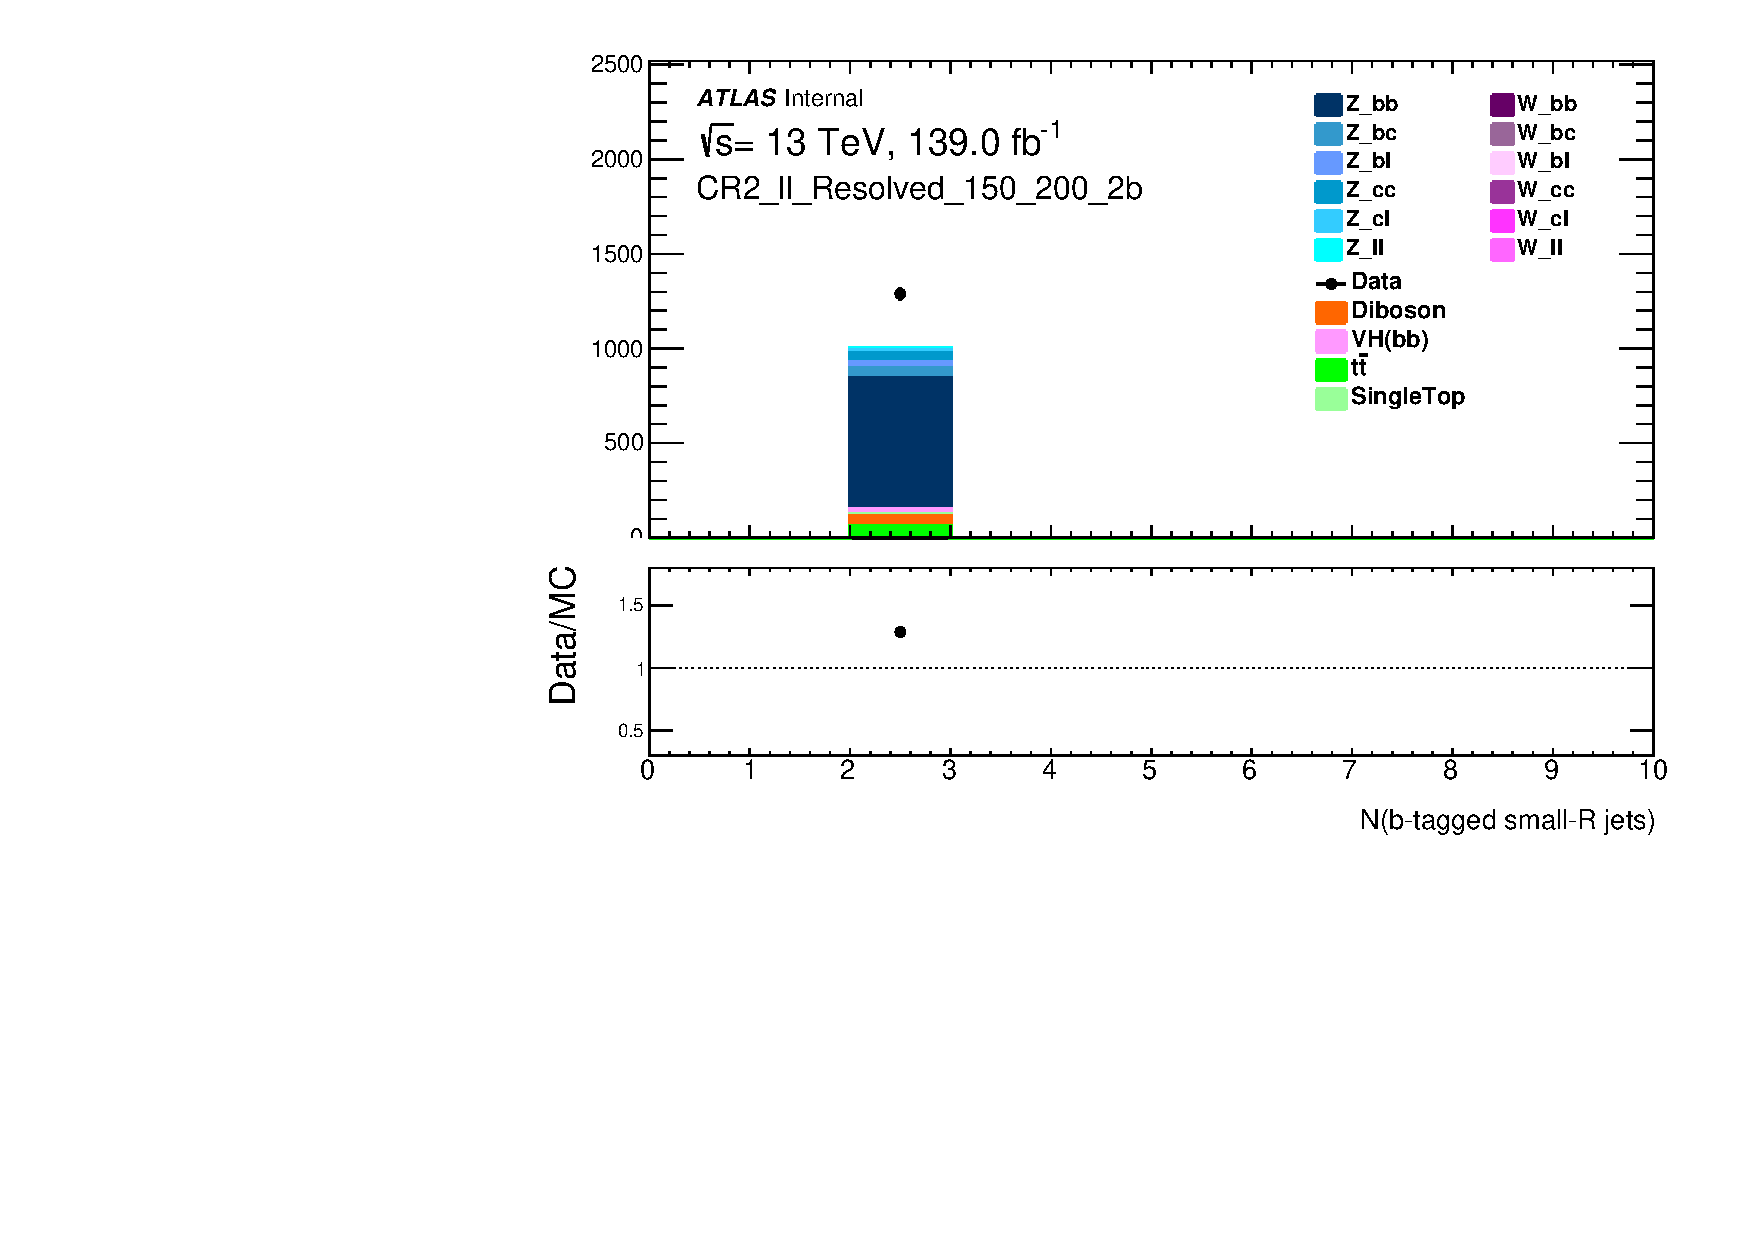
\includegraphics[width=0.46\linewidth]{chapters/c8/figures/2L/DataMC_MonoH_Nominal_CR2_ll_Resolved_150_200_2b_N_BJets_04.pdf}
    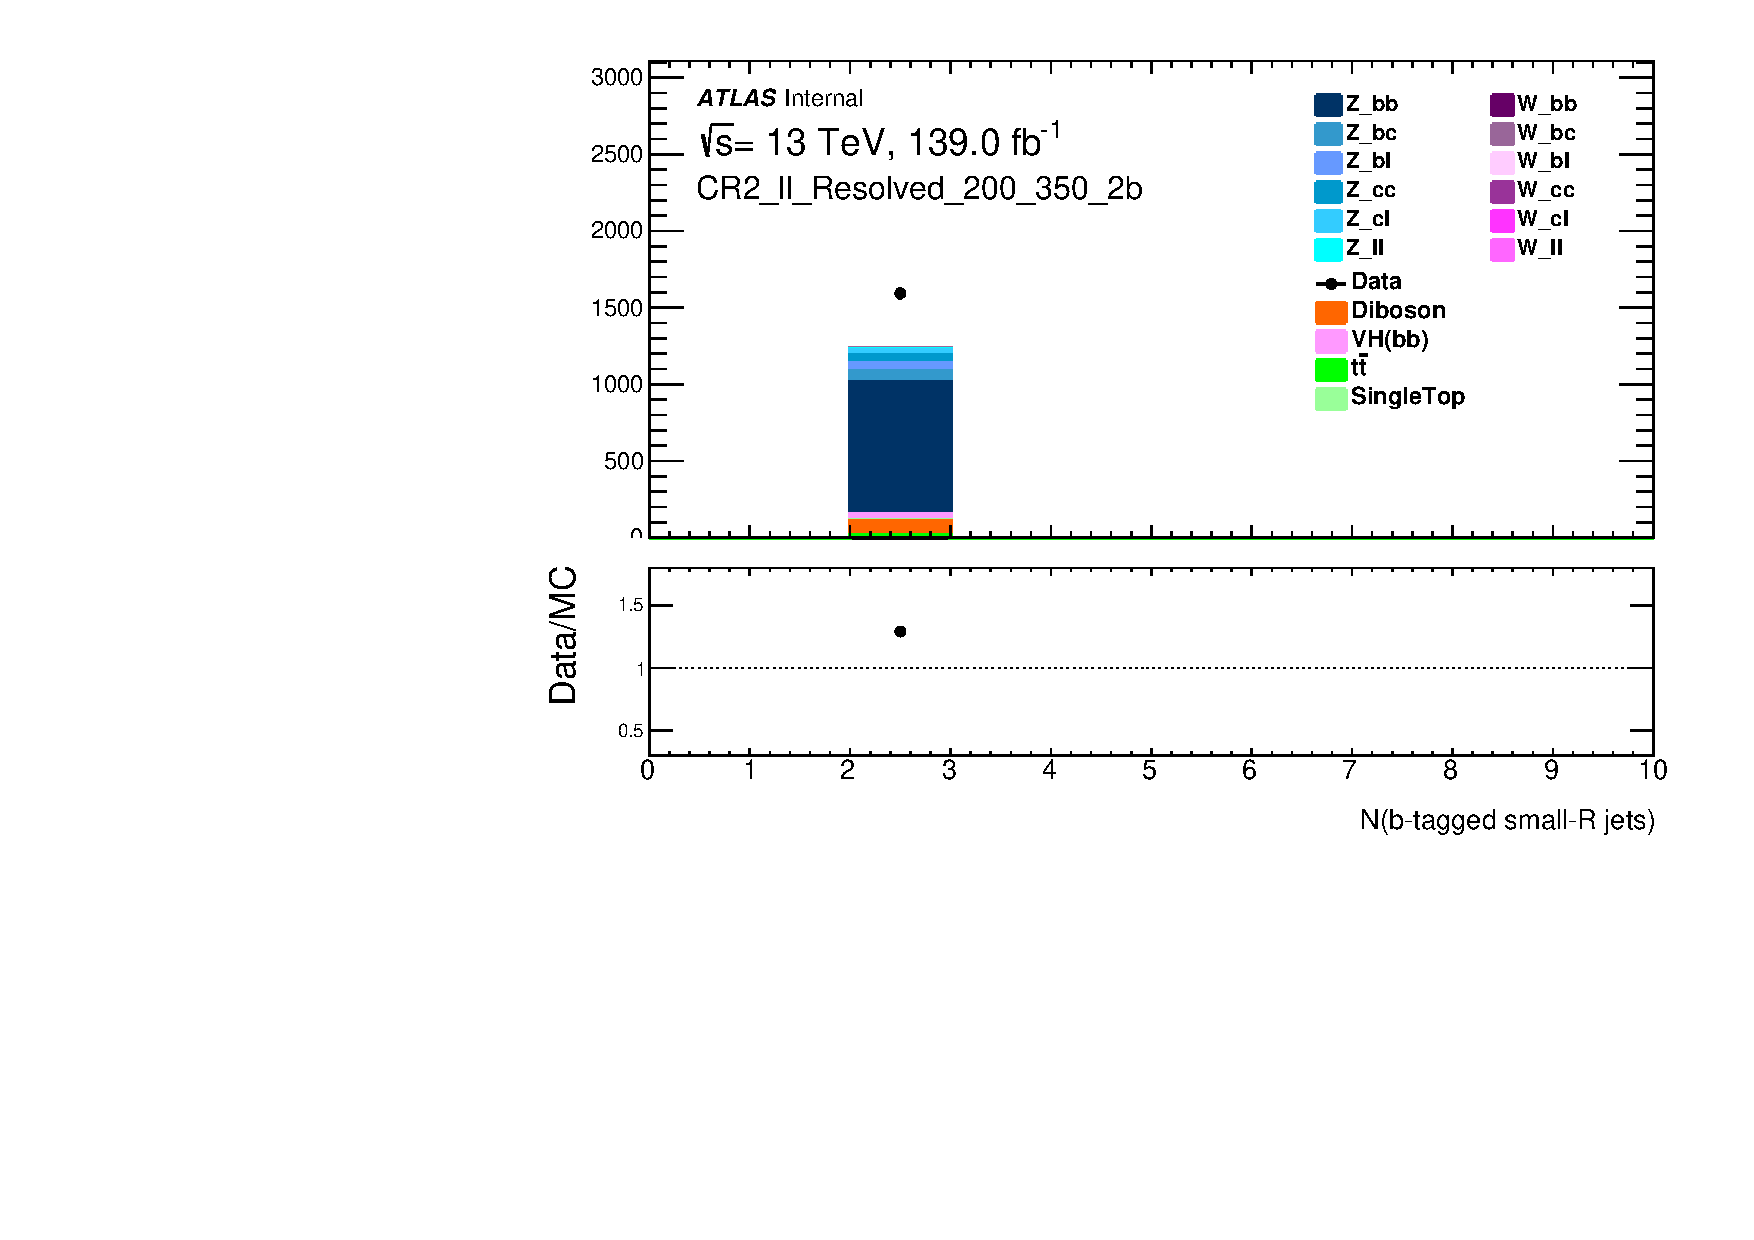
\includegraphics[width=0.46\linewidth]{chapters/c8/figures/2L/DataMC_MonoH_Nominal_CR2_ll_Resolved_200_350_2b_N_BJets_04.pdf}\\
    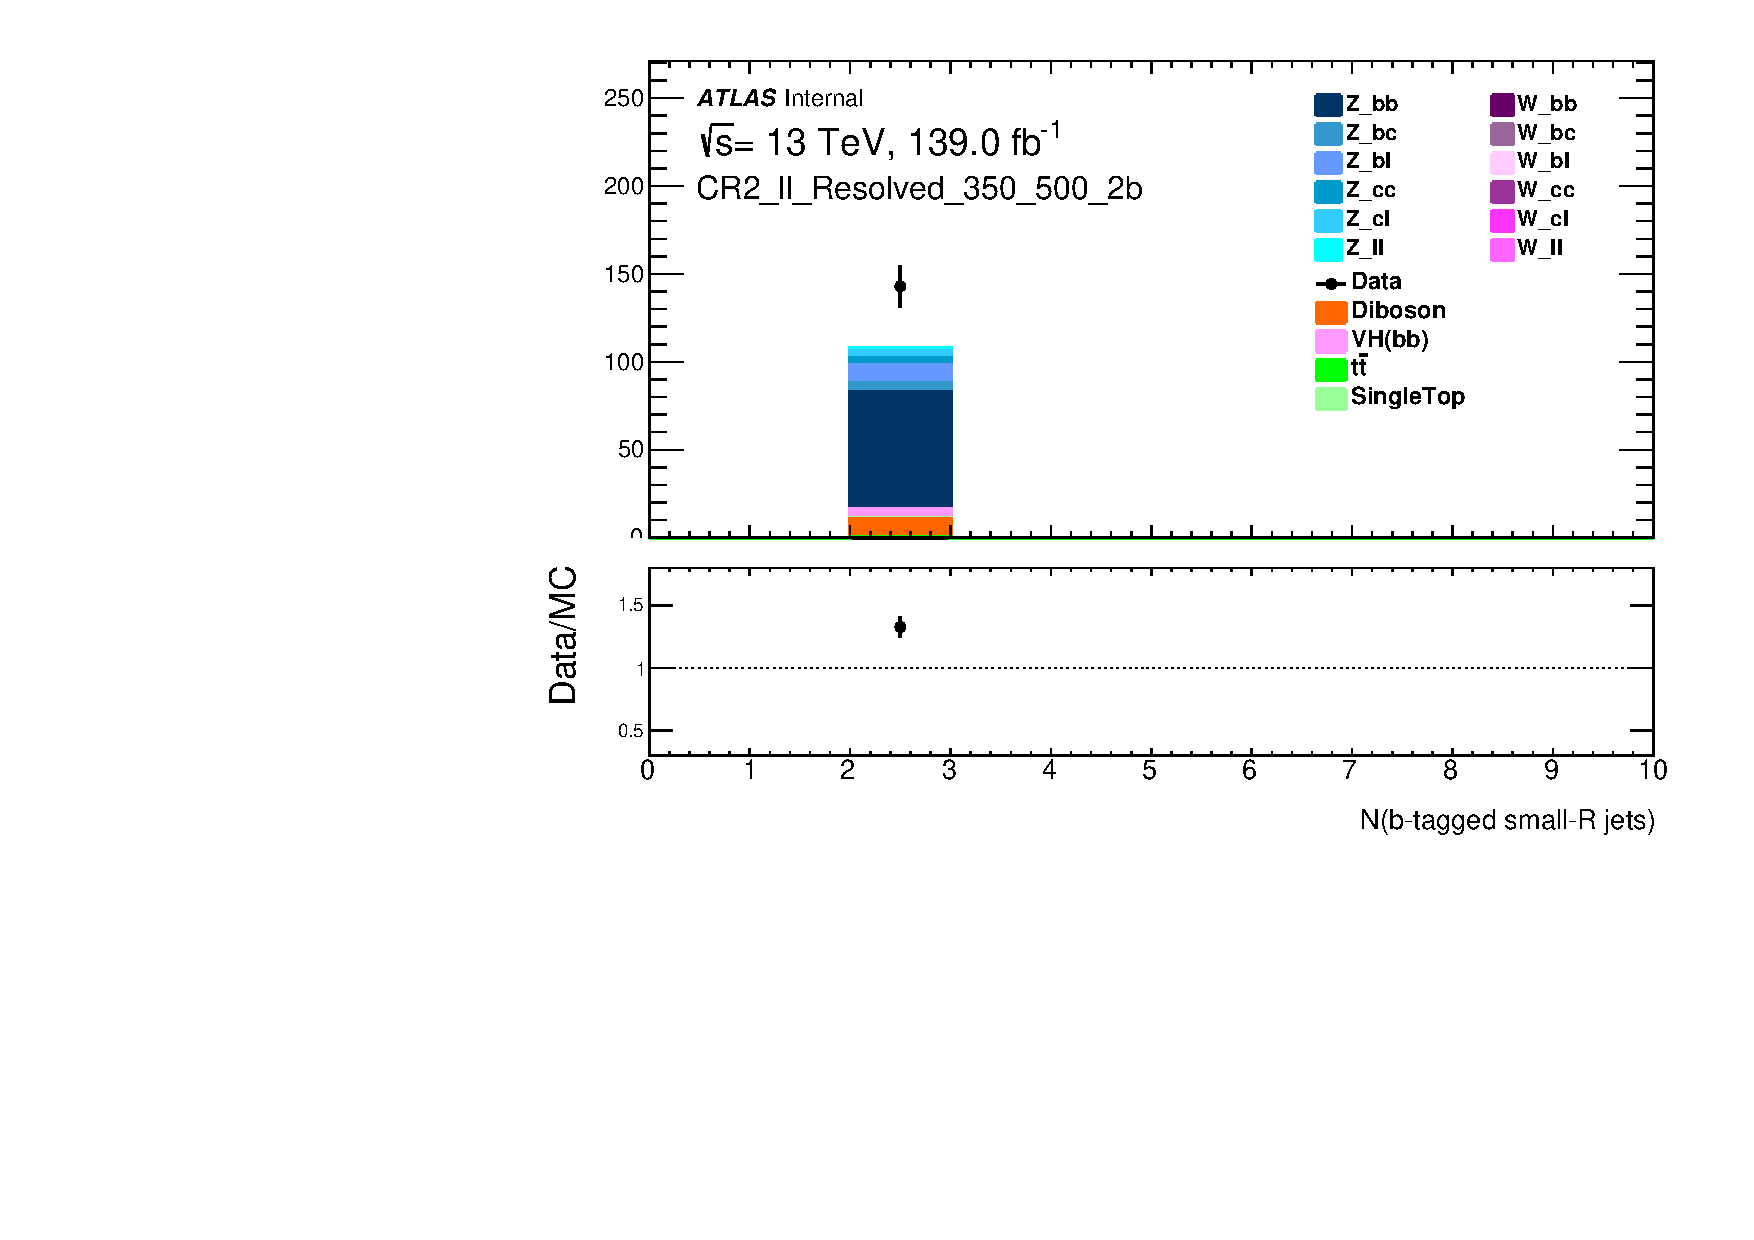
\includegraphics[width=0.46\linewidth]{chapters/c8/figures/2L/DataMC_MonoH_Nominal_CR2_ll_Resolved_350_500_2b_N_BJets_04.pdf}
    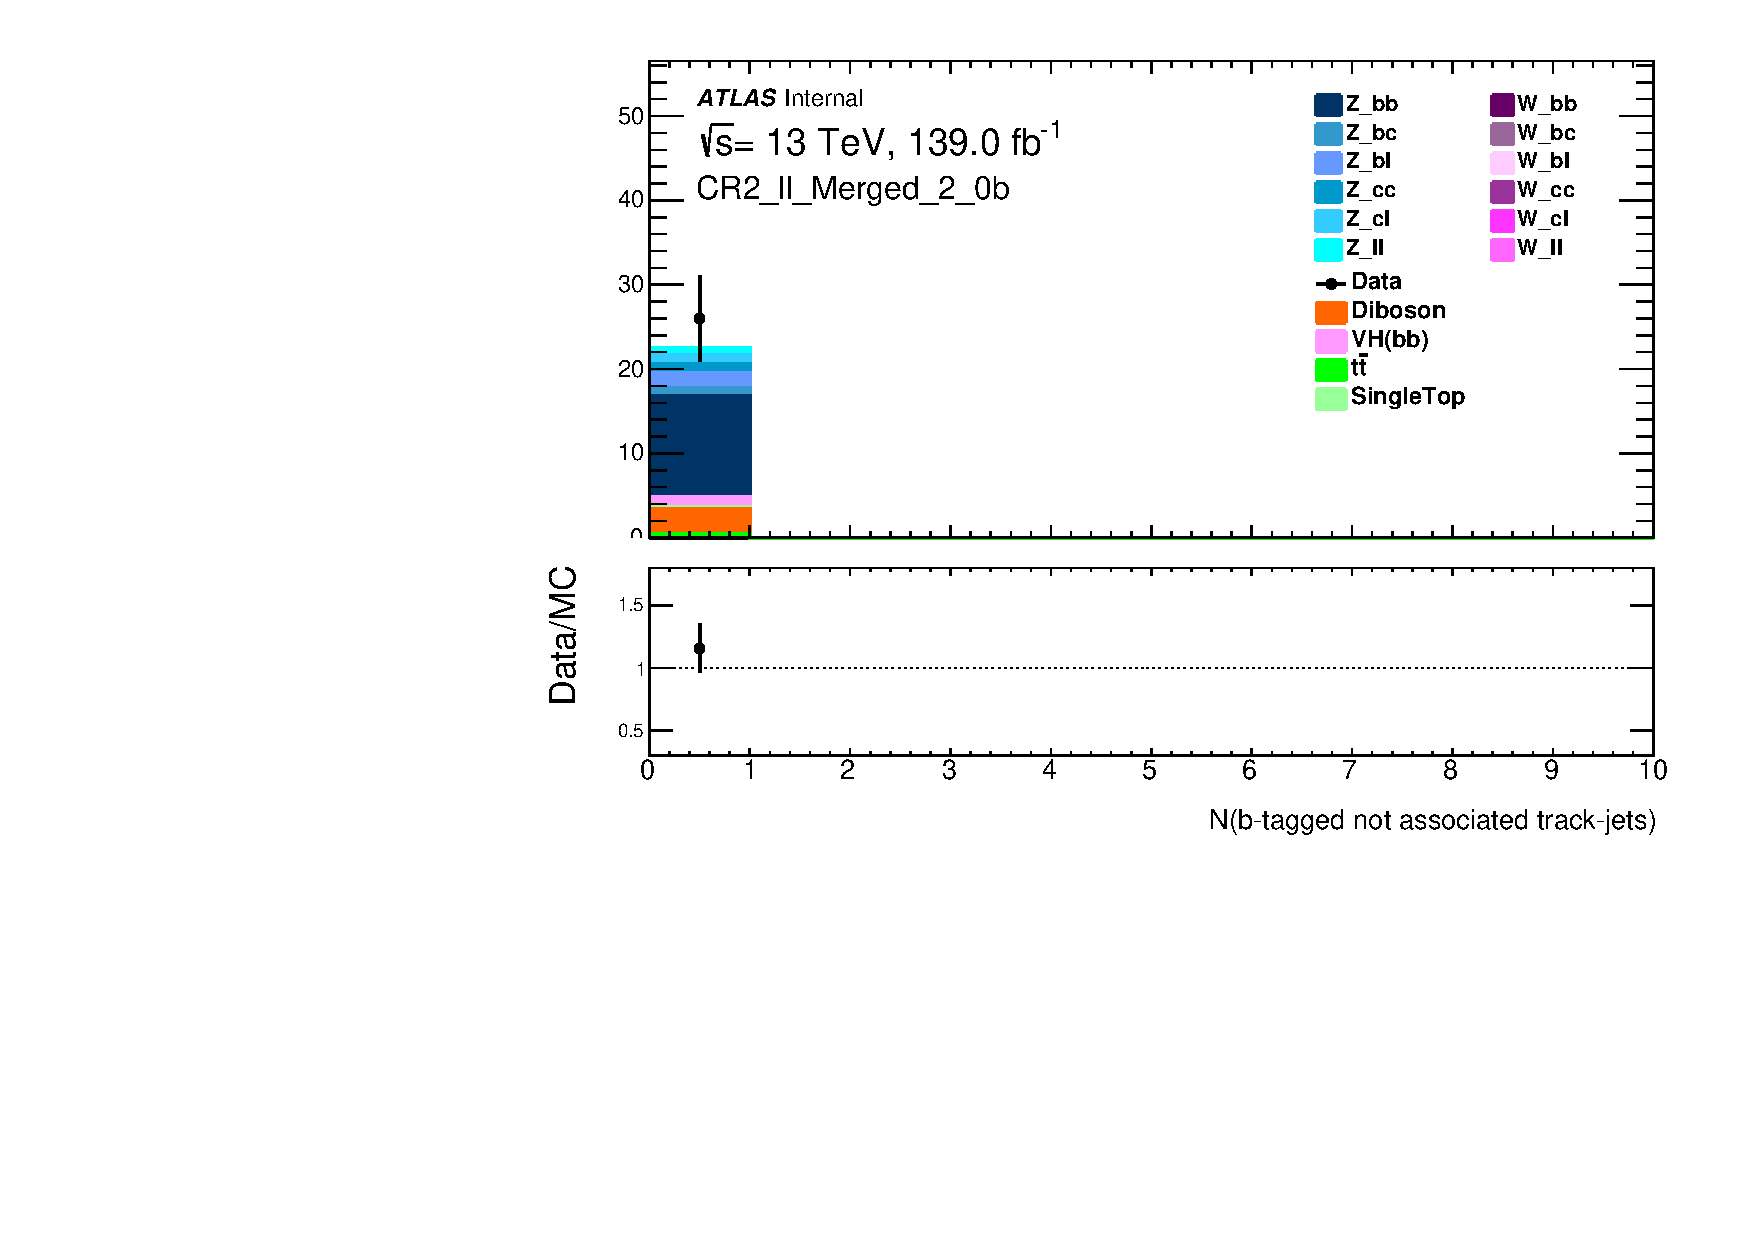
\includegraphics[width=0.46\linewidth]{chapters/c8/figures/2L/DataMC_MonoH_Nominal_CR2_ll_Merged_2_0b_N_BTags_not_associated_02.pdf}
    \caption{Total yields in the 2-lepton control region for different \met~regions with 2 $b$-tagged jets.}
    \label{fig:data-mc-2l-ll-nb-2b}
\end{figure}
  
\begin{figure}[!htb]
    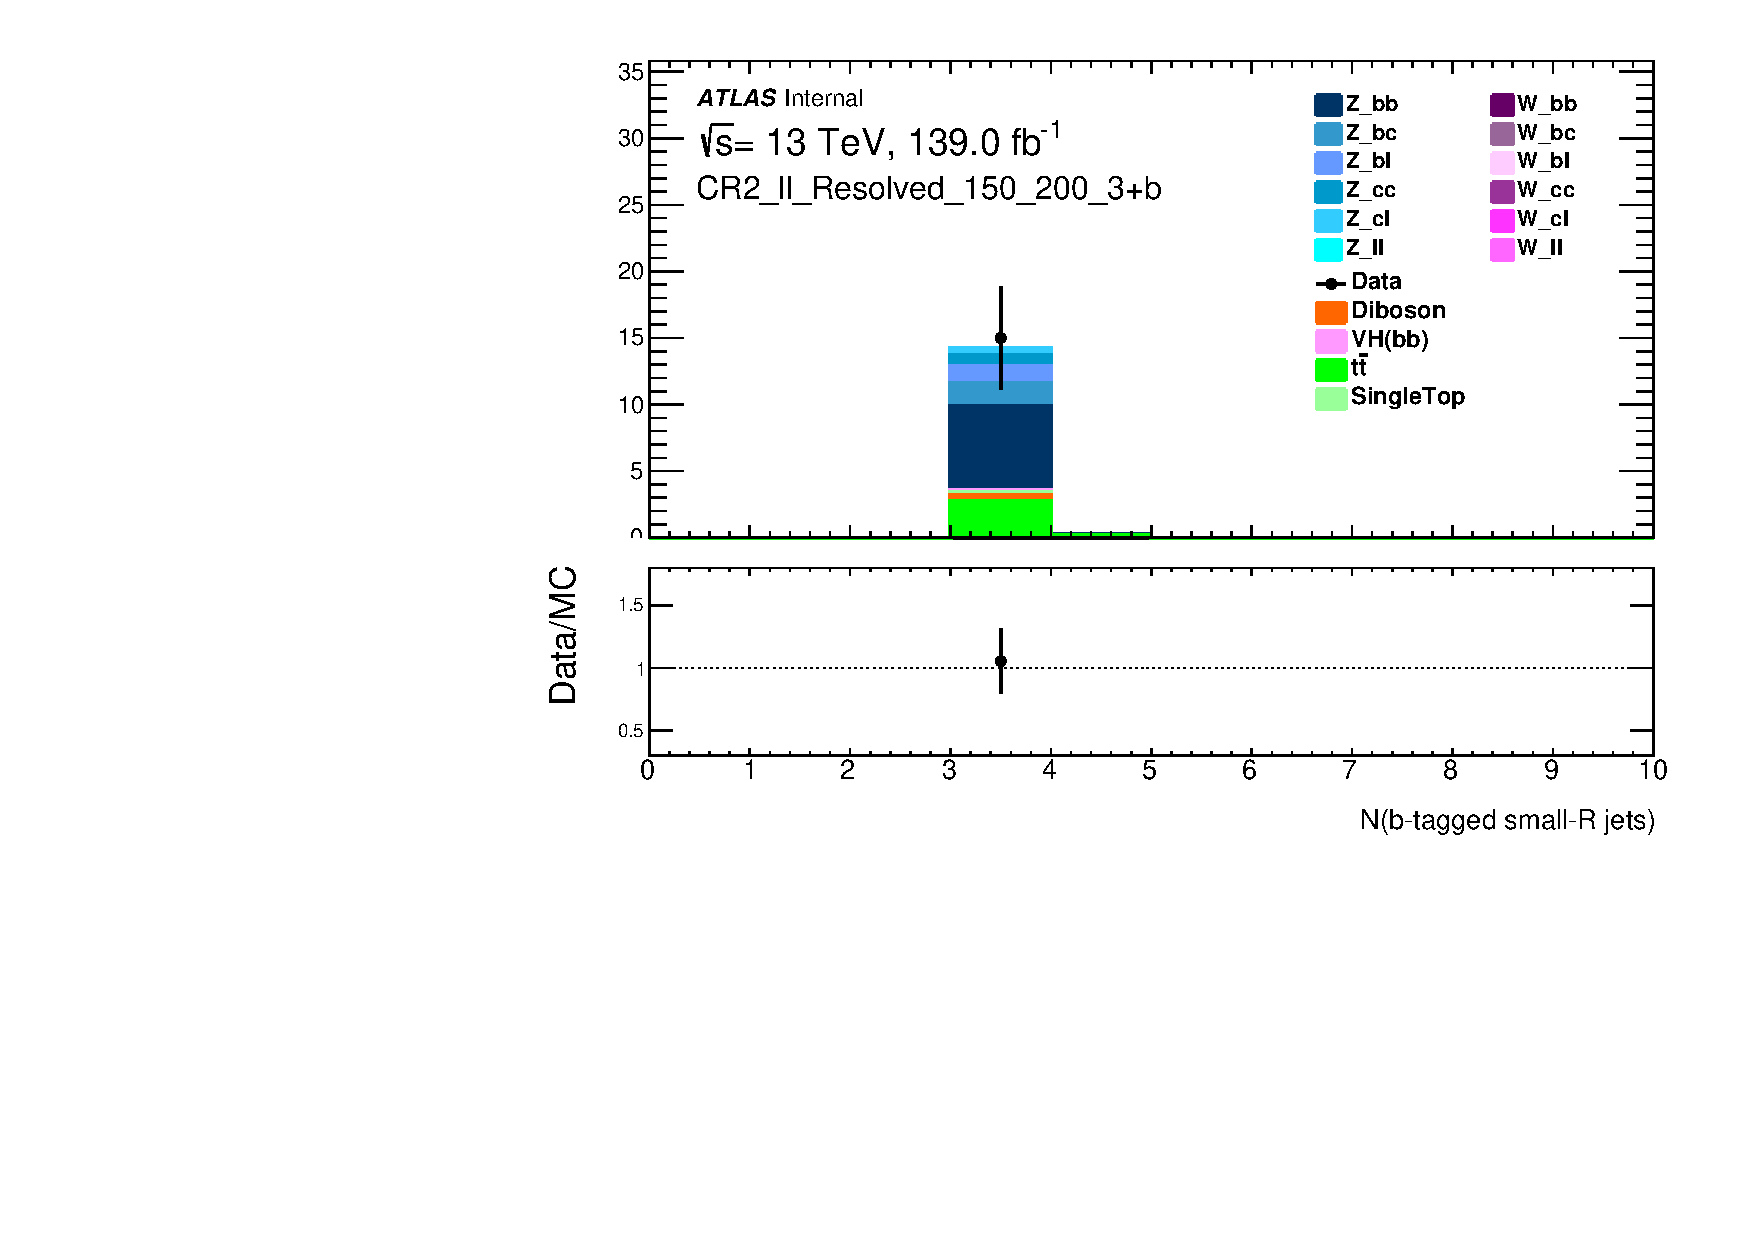
\includegraphics[width=0.46\linewidth]{chapters/c8/figures/2L/DataMC_MonoH_Nominal_CR2_ll_Resolved_150_200_3+b_N_BJets_04.pdf}
    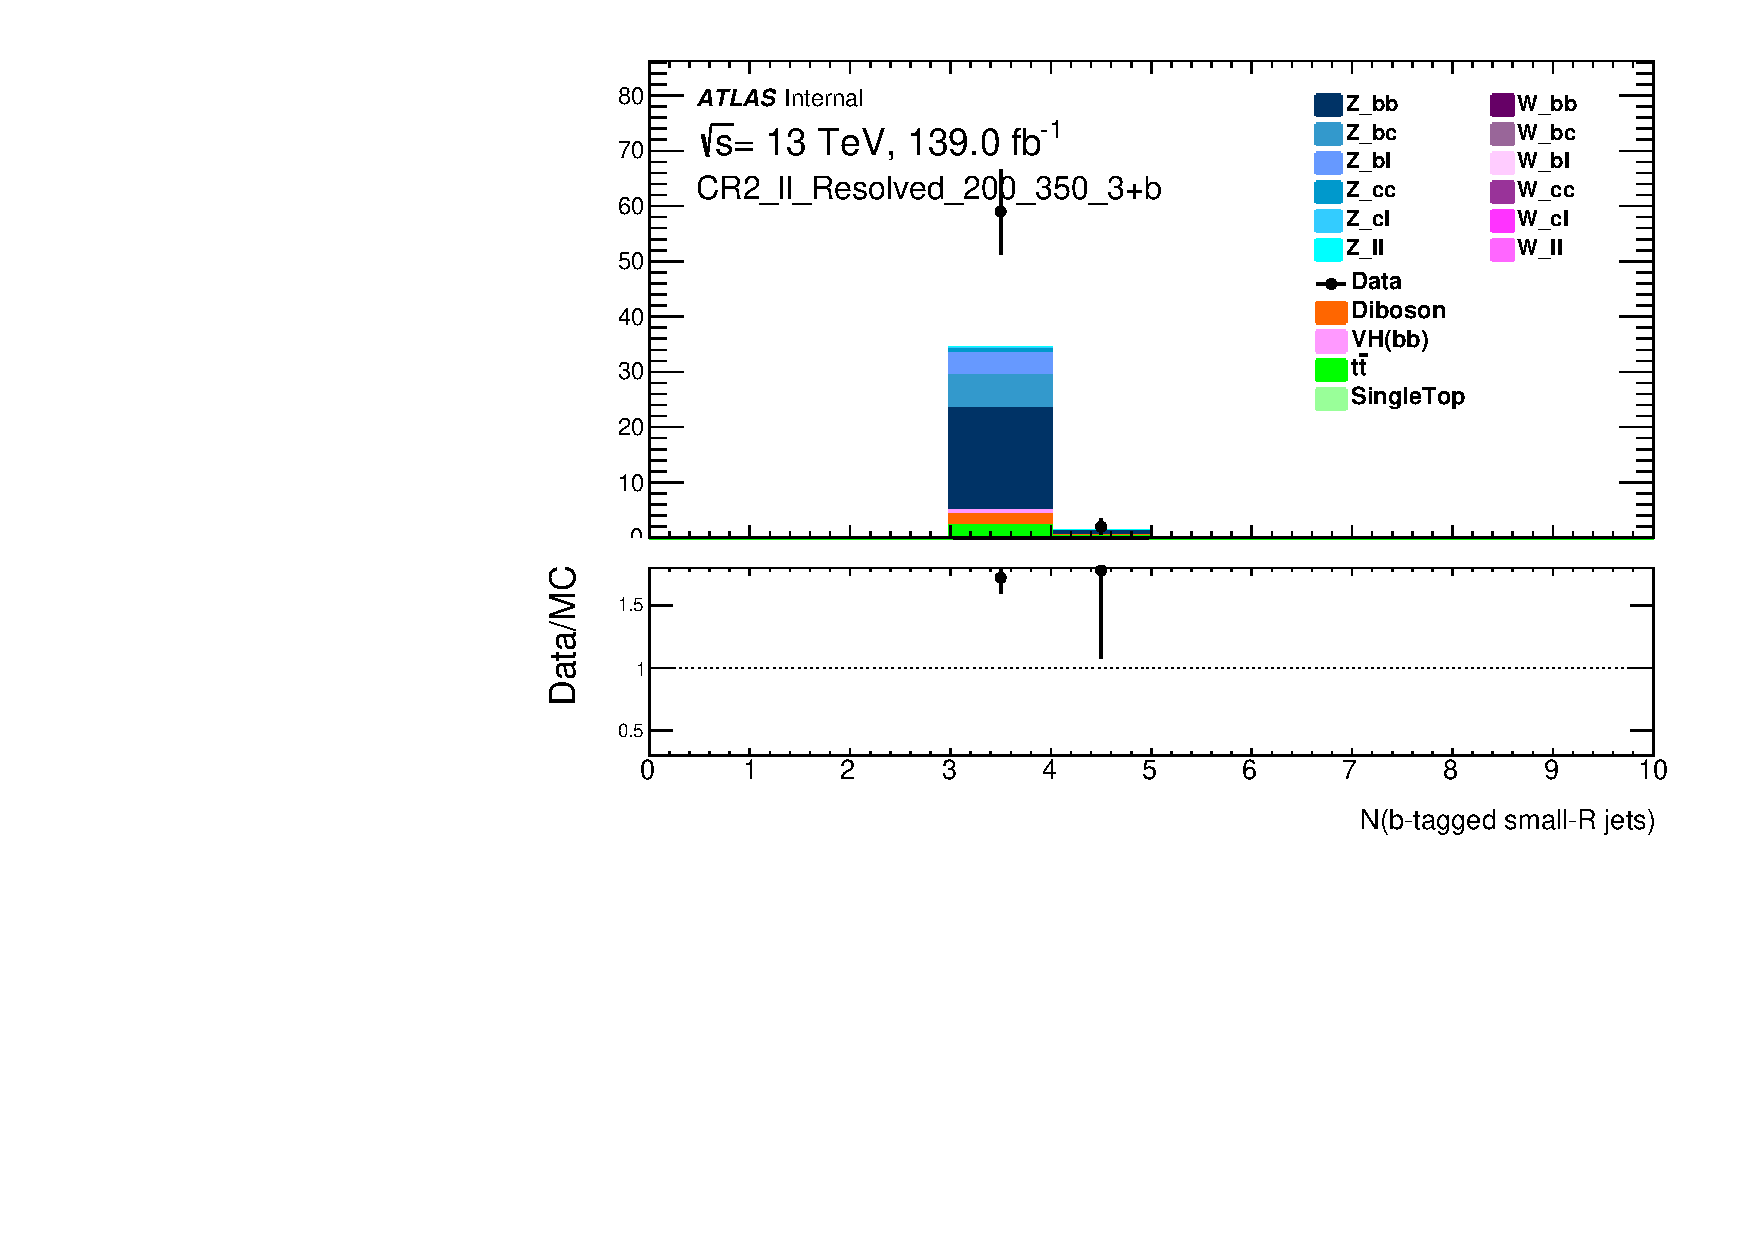
\includegraphics[width=0.46\linewidth]{chapters/c8/figures/2L/DataMC_MonoH_Nominal_CR2_ll_Resolved_200_350_3+b_N_BJets_04.pdf}\\
    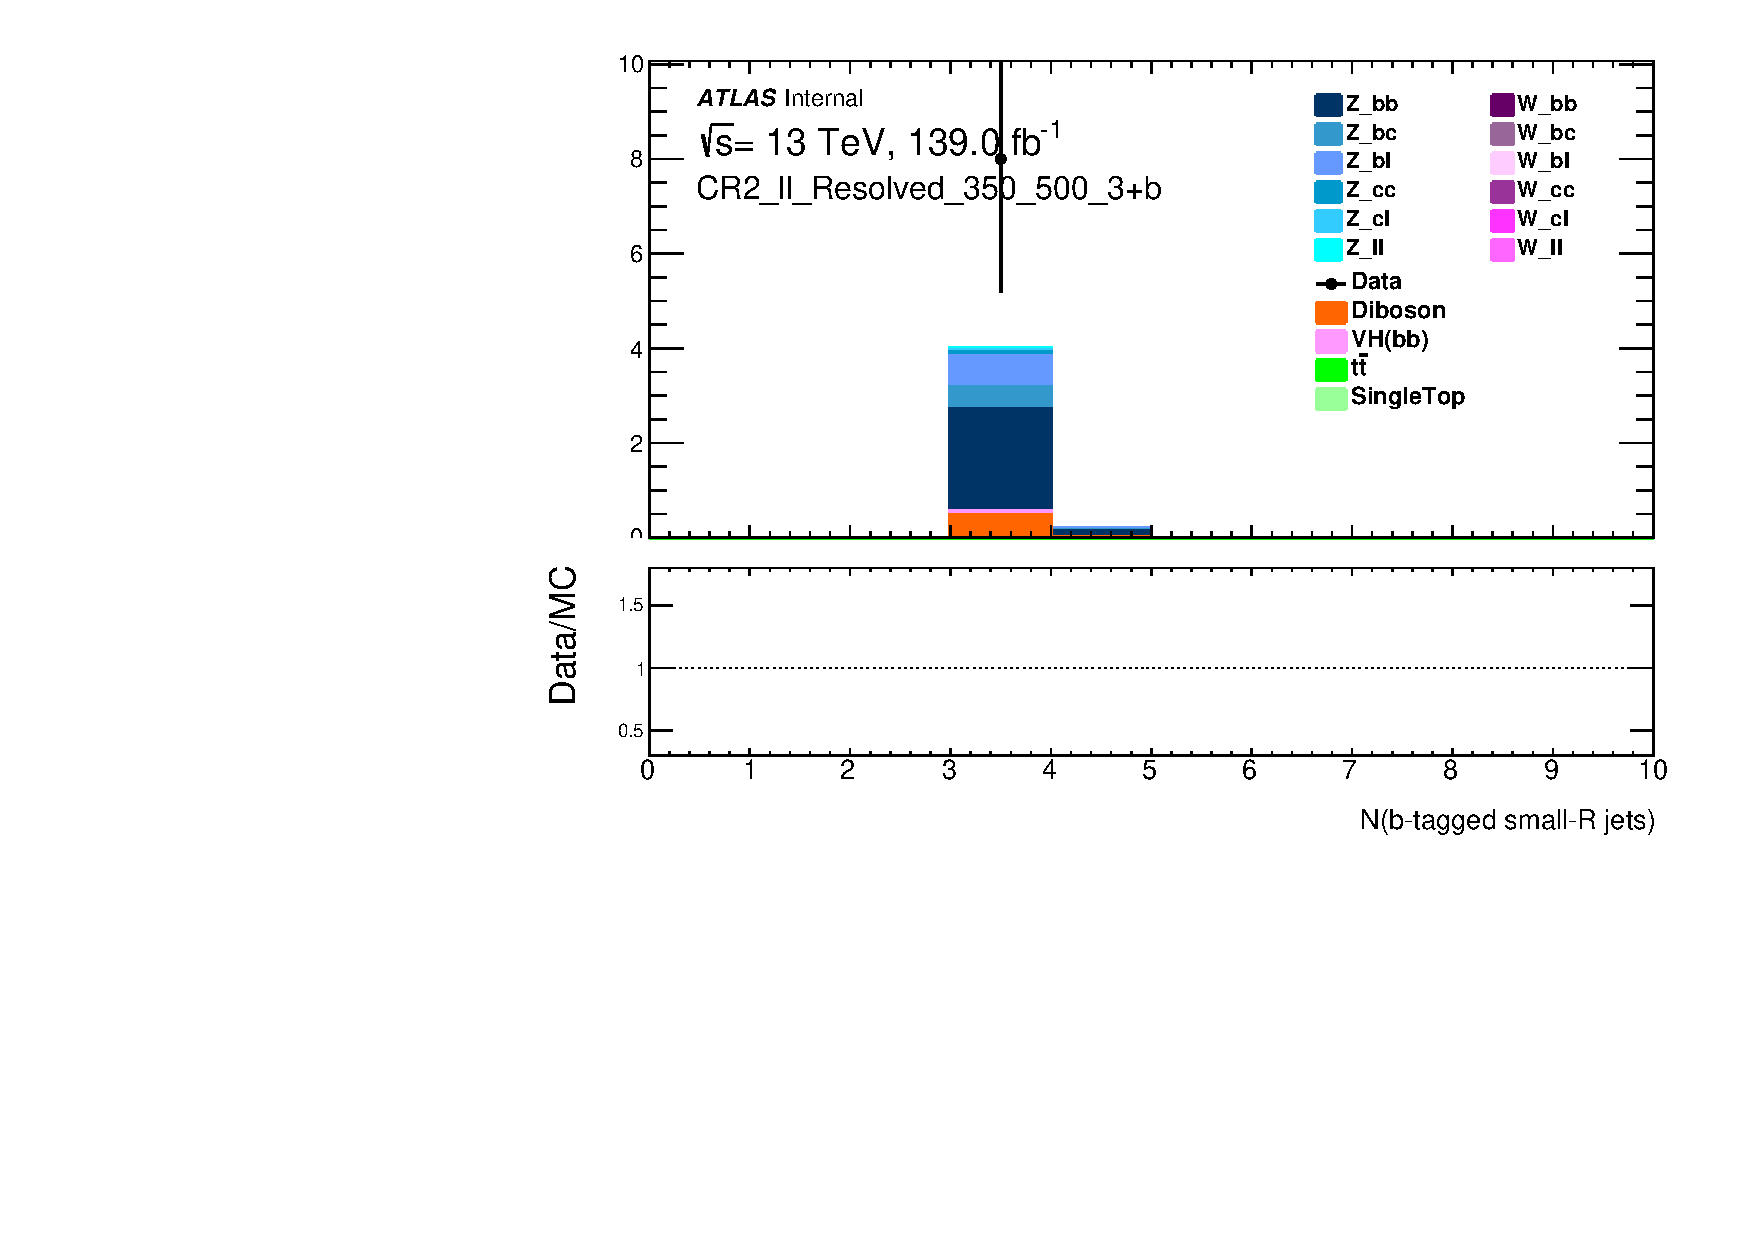
\includegraphics[width=0.46\linewidth]{chapters/c8/figures/2L/DataMC_MonoH_Nominal_CR2_ll_Resolved_350_500_3+b_N_BJets_04.pdf}
    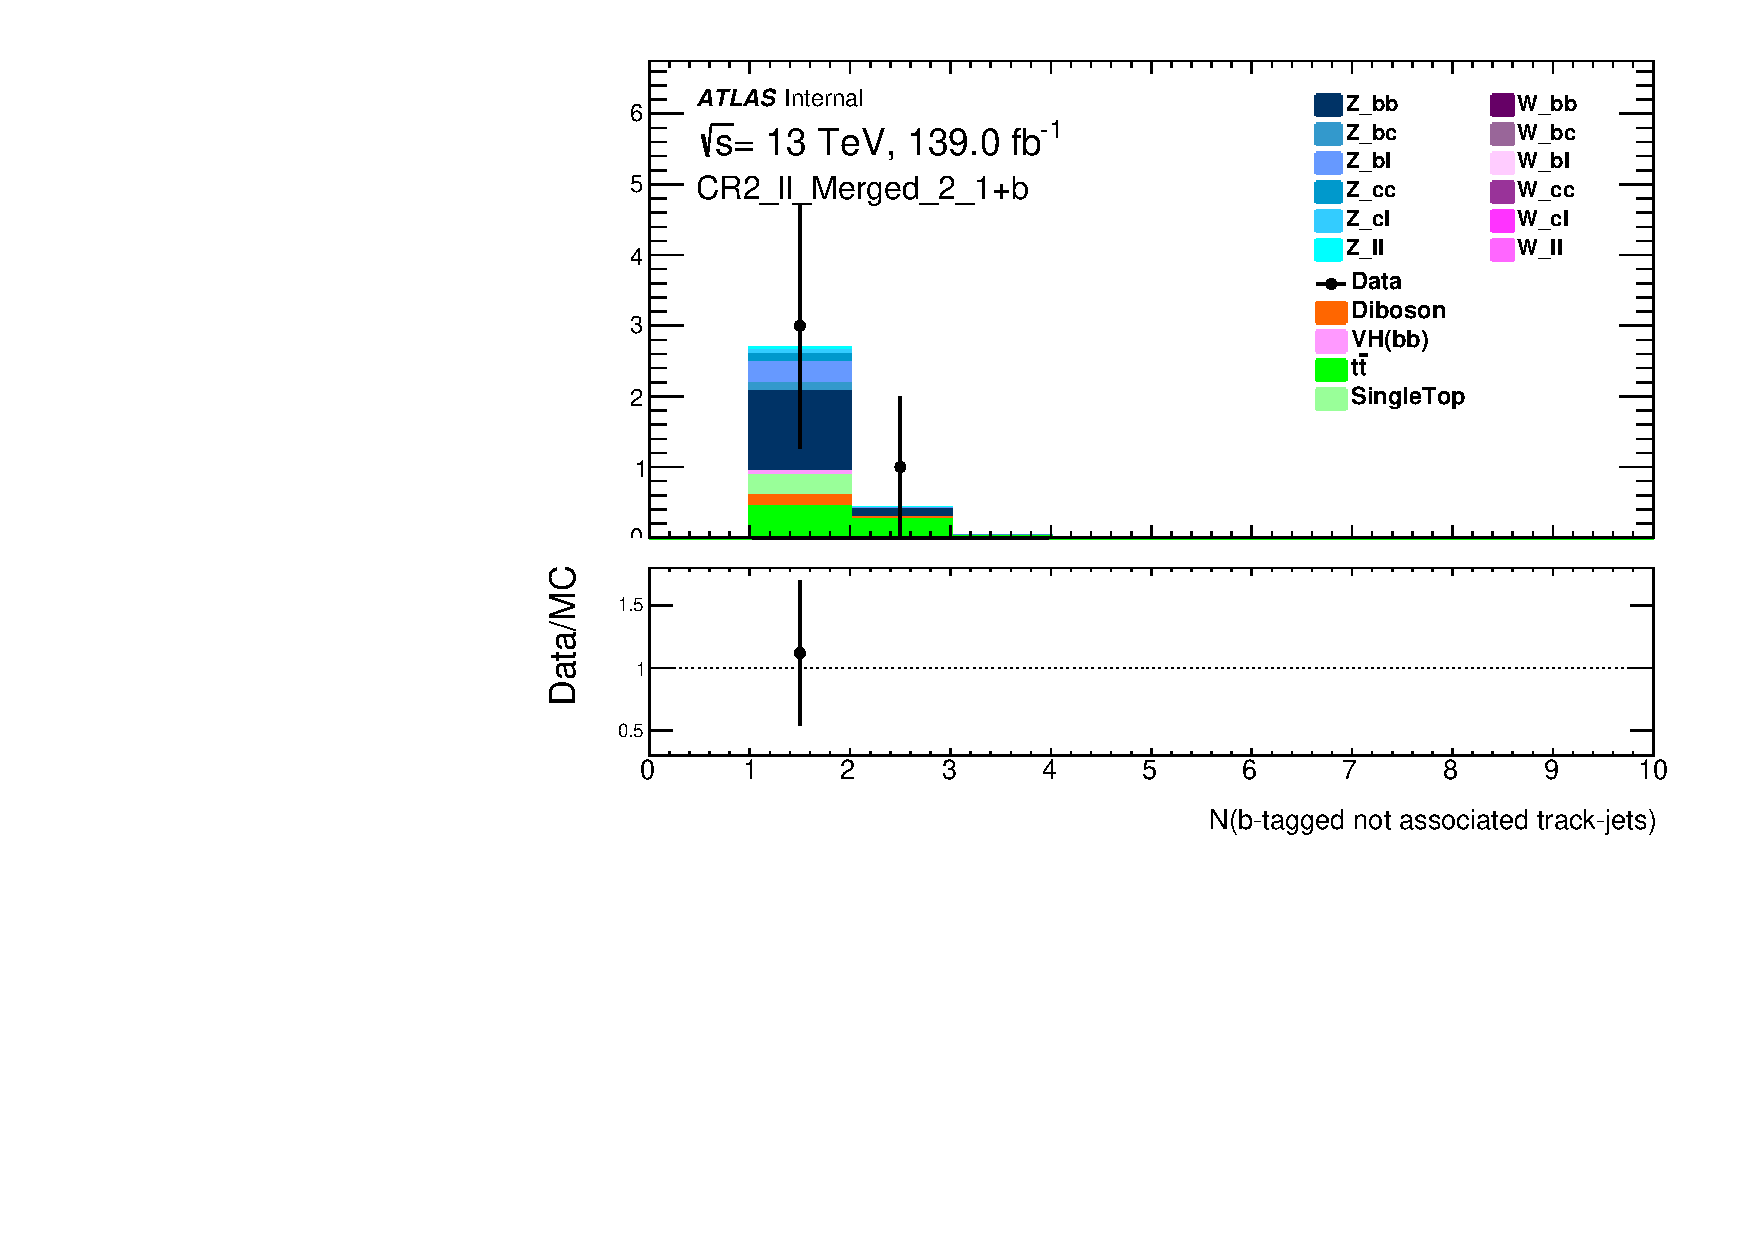
\includegraphics[width=0.46\linewidth]{chapters/c8/figures/2L/DataMC_MonoH_Nominal_CR2_ll_Merged_2_1+b_N_BTags_not_associated_02.pdf}
    \caption{Total yields in the 2-lepton control region for different \met~regions with more than 2 $b$-tagged jets.}
    \label{fig:data-mc-2l-ll-nb-3+b}
\end{figure}

\chapter{Statistical analysis}
\label{ch:stat-ana}

\par Statistical analysis is a process to analyze collision data in the signal and control regions with statistical models to test physics hypothesis. 
In new physics search analysis, one can do hypothesis testing on new physics if relatively obvious excesses are observed in data versus Monte-Carlo background comparison plots. 
In this analysis, since the no obvious excesses happen, model exclusion becomes a meaningful target to achieve. 
New physics model exclusion with collision data can be turned viewed as parameters confidential interval estimation. 
In particle physics, the CLs method\cite{Read:2002hq} is a powerful and proven method for model parameters limit setting. 
In this chapter, the CLs strategies for this analysis are described in Section~\ref{sec:cls}, and then, the fit results are demonstrated in Section~\ref{sec:limitres}. 

\section{CLs method}
\label{sec:cls}

\par The aim of statistical analysis is to evaluate the upper limit of new physics model parameters , for example, mass of z prime in 2HDM model, given observation and nuisance parameters. 
Confidence interval is associated with a confidence level that the true parameter is in the proposed range. 
The CLs method, which is a statistical estimation to evaluate confidence interval of parameters of a model with data, is the approach that used to set the upper limit of new physics model parameters in this analysis.

\par The CLs method is not the only approach to set the upper limit of model parameters. 
One can also use the traditional frequentist approach or novel Bayesian way instead. 
The Bayesian way is not preferred by experimental physicists because it needs to set a prior on the new physics model itself.
The traditional frequentist approach has trouble when the signal is too small. 
It will give a negative upper limit since it estimates data yield with confidence level, then subtract background yield.
Therefore, the CLs method, as a modified frequentist approach, is introduced with a normalization on background only probability to avoid this issue.

\par Like all other upper limit estimation approaches, one needs to build likelihood function first, count data and background yields in different event categories, and deal with the nuisance parameters to get limit setting result. 
More details will be covered in the rest of this section.

\subsection{Likelihood definition}

\par The likelihood function is a reflection of probability of event yields in signal region. 
It is obvious that the event count in the signal region follows Poisson distribution, since each event have a finite probability to be observed in the signal region.
Therefore, the statistical analysis of the data uses a binned likelihood function constructed as the product of Poisson probability terms,
\begin{equation}
\mathrm{Poisson}\,(n|\mu S+B)\left[ \prod_{b\in \text{bins}}^{n} \frac{\mu \nu^{\mathrm{sig}}_{b}+\nu^{\mathrm{bkg}}_{b}}{\mu S+B} \right],
\end{equation}
where $\mu$, a signal strength parameter, multiplies the expected signal yield $\nu^{\mathrm{sig}}_b$ in each histogram bin $b$, and $\nu^{\mathrm{bkg}}_b$ represents the background content for bin $b$. 
The dependence of the signal and background predictions on the systematic uncertainties is described by a set of nuisance parameters (NP) $\theta$, which are parameterized by Gaussian or log-normal priors. 
The latter are used for normalization uncertainties in order to maintain a positive likelihood.

\par This profile of likelihood, together with Monte-Carlo simulation of signal and background, are used to model the data yields.

\subsection{Nuisance parameters}

\par In statistics, nuisance parameters are the parameters which are not of immediate interest but which must be accounted for in the analysis of those parameters which are of interest. 
Two types of nuisance parameters are considered in this analysis:
\begin{itemize}
    \item \textbf{Normalization related nuisance parameters}: These nuisance parameters are single number correction that comes from cross-section calculation, Monte-Carlo template and relative acceptance, etc.. 
    A full list of normalization of this type nuisance parameters are shown in Table~\ref{tab:np-norm1} and~\ref{tab:np-norm2}.
    \item \textbf{Shape related nuisance parameters}: These nuisance parameters are introduced by either detector or theory, and will be used to fit observables. 
    A full list of normalization of this type nuisance parameters are shown in Table~\ref{tab:np-shape1} and~\ref{tab:np-shape2}.
\end{itemize}

\begin{table}[ht]
    \centering
    \scriptsize
    \begin{tabular}{|p{2.5cm}|p{1.5cm}|p{3cm}|p{2.5cm}|p{1.5cm}|}
        \hline
        NP Name & Prior & Description & Applied to sample & Applied in region \\
        \hline
        \texttt{norm\_Zhf} & flat & normalisation of Zhf template & Zhf & all \\
        \texttt{norm\_Whf} & flat & normalisation of Whf template & Zhf & all \\
        \texttt{norm\_ttbar} & flat & normalisation of $t\bar{t}$ template & $t\bar{t}$ & all \\
        \hline
        \hline
        \texttt{stopsNorm} & 3.7\% & single top $s$-channel inclusive normalisation & $s$-channel s.top & all \\
        \texttt{stoptNorm} & 3.9\% & single top $t$-channel inclusive normalisation & $t$-channel s.top & all \\
        \texttt{stopWtNorm} & 5.4\% & single top $Wt$-channel inclusive normalisation & $Wt$-channel s.top & all \\
        \texttt{WWNorm} & 25\% & inclusive normalisation of $WW$ & WW & all \\
        \texttt{WZNorm} & 26\% & inclusive normalisation of $WZ$ & WZ & all \\
        \texttt{ZZNorm} & 20\% & inclusive normalisation of $ZZ$ & ZZ & all \\
        \texttt{HiggsNorm} & 22\% & inclusive normalisation of SM $Vh(b\bar{b})$ & VHbb & all \\
        \hline
        \hline
        \texttt{ZcllNorm} & 30\% & inclusive normalisation uncertainty for $Zcl$ & Zcl & all \\
        \texttt{WcllNorm} & 30\% & inclusive normalisation uncertainty for $Wcl$ & Zcl & all \\
        \texttt{ZlNorm} & 10\% & inclusive normalisation uncertainty for $Zl$ & Zl & all \\
        \texttt{WlNorm} & 10\% & inclusive normalisation uncertainty for $Wl$ & Wl & all \\
        \hline
        \hline
        \texttt{ZhfNorm\_L0} & 20\% & relative acceptance difference of Zhf between 0 and 2L regions & Zhf & 0L \\
        \texttt{WhfNorm\_L0} & 20\% & relative acceptance difference of Zhf between 0 and 2L regions & Whf & 0L \\
        \hline
    \end{tabular}
    \caption{Nuisance parameters associated to theoretical uncertainties that affect the normalisation/relative acceptance with their prior uncertainties (in the case of Gaussian priors the numbers correspond to the $1\sigma$ prefit uncertainties).}
    \label{tab:np-norm1}
\end{table}

\begin{table}[ht]
    \centering
    \scriptsize
    \begin{tabular}{|p{2.5cm}|p{1.5cm}|p{3cm}|p{2.5cm}|p{1.5cm}|}
        \hline
        NP Name & Prior & Description & Applied to sample & Applied in region \\
        \hline
        \texttt{WblWhfRatio} & 20\% & uncertainty on $\sigma(Wbl)$/$\sigma(Whf)$ & Wbl & 0L, 1L \\
        \texttt{WccWhfRatio} & 20\% & uncertainty on $\sigma(Wcc)$/$\sigma(Whf)$ & Wcc & 0L, 1L \\
        \texttt{WbcWhfRatio} & 20\% & uncertainty on $\sigma(Wbc)$/$\sigma(Whf)$ & Wbc & 0L, 1L \\
        \texttt{ZblZhfRatio} & 20\% & uncertainty on $\sigma(Zbl)$/$\sigma(Zhf)$ & Zbl & all \\
        \texttt{ZccZhfRatio} & 20\% & uncertainty on $\sigma(Zcc)$/$\sigma(Zhf)$ & Zcc & all \\
        \texttt{ZbcZhfRatio} & 20\% & uncertainty on $\sigma(Zbc)$/$\sigma(Zhf)$ & Zbc & all \\
        \hline
        \hline
        \texttt{SysTopMETshape} & 20\% & relative acceptance difference across \met bins & $t\bar{t}$ & all except lowest \met bin \\
        \texttt{SysWhfMETshape} & 20\% & relative acceptance difference across \met bins & Whf & all except lowest \met bin \\
        \texttt{SysZhfMETshape} & 20\% & relative acceptance difference across \met bins & Zhf & all except lowest \met bin \\
        \hline
        \hline
        \texttt{ATLAS\_LUMI} & 1.7\% & luminosity uncertainty & all & all \\
        \hline
    \end{tabular}
    \caption{Nuisance parameters associated to theoretical uncertainties that affect the normalisation or relative acceptance with their prior uncertainties (in the case of Gaussian priors the numbers correspond to the $1\sigma$ prefit uncertainties).}
    \label{tab:np-norm2}
\end{table}

\begin{table}[ht]
    \centering
    \scriptsize
    \begin{tabular}{|p{3.5cm}|p{2.5cm}|p{1.5cm}|p{2cm}|p{1.5cm}|}
        \hline
        NP Name & Description & Treatment & Applied to sample & Applied in region \\
        \hline
        \texttt{SysttbarMbb} & Sec.~\ref{sec:thy-sys-unc} & - & $t\bar{t}$ & all \\
        \texttt{SysttbarMbb} & Sec.~\ref{sec:thy-sys-unc} & - & single-top $Wt$ & all \\
        \texttt{SysWMbb} & Sec.~\ref{sec:thy-sys-unc} & - & Whf, Wcl, Wl & all \\
        \texttt{SysZMbb} & Sec.~\ref{sec:thy-sys-unc} & - & Zhf, Zcl, Zl & all \\
        \texttt{SysWWMbb} & Sec.~\ref{sec:thy-sys-unc} & - & WW & all \\
        \texttt{SysWZMbb} & Sec.~\ref{sec:thy-sys-unc} & - & WZ & all \\
        \texttt{SysZZMbb} & Sec.~\ref{sec:thy-sys-unc} & - & ZZ & all \\
        \hline
    \end{tabular}
    \caption{Nuisance parameters associated to theoretical uncertainties that affect the $m(b\bar{b})$ shape and their treatment (S=smoothed, Sym1=symmetrised (one-sided systematic), Sym2=symmetrised (two-sided systematic)).}
    \label{tab:np-shape1}
\end{table}

\begin{table}[ht]
    \centering
    \scriptsize
    \begin{tabular}{|p{3.5cm}|p{2.0cm}|p{1.5cm}|p{2cm}|p{1.5cm}|}
        \hline
        NP Name & Description & Treatment & Applied to sample & Applied in region \\
        \hline
        \texttt{EL\_EFF\_*} & Sec.~\ref{sec:exp-sys-unc} & - & all & all \\
        \texttt{EG\_RESOLUTION\_*} & Sec.~\ref{sec:exp-sys-unc} & S & all & all \\
        \texttt{EG\_SCALE\_*} & Sec.~\ref{sec:exp-sys-unc} & S & all & all \\
        \texttt{MUON\_EFF\_*} & Sec.~\ref{sec:exp-sys-unc} & - & all & all \\
        \texttt{MUON\_SAGITTA\_*} & Sec.~\ref{sec:exp-sys-unc} & - & all & all \\
        \texttt{MUON\_SCALE\_*} & Sec.~\ref{sec:exp-sys-unc} & S & all & all \\
        \texttt{MUON\_MS\_*} & Sec.~\ref{sec:exp-sys-unc} & S & all & all \\
        \texttt{MUON\_ID\_*} & Sec.~\ref{sec:exp-sys-unc} & S & all & all \\
        \texttt{TAUS\_TRUEELECTRON\_*} & Sec.~\ref{sec:exp-sys-unc} & - & all & all \\
        \texttt{TAUS\_TRUEHADTAU\_EFF\_*} & Sec.~\ref{sec:exp-sys-unc} & - & all & all \\
        \texttt{TAUS\_TRUEHADTAU\_SME\_*} & Sec.~\ref{sec:exp-sys-unc} & S & all & all \\
        \texttt{JET\_EffectiveNP\_*} & Sec.~\ref{sec:exp-sys-unc} & S, Sym2 & all & all \\
        \texttt{JET\_Eta*} & Sec.~\ref{sec:exp-sys-unc} & S, Sym2 & all & all \\
        \texttt{JET\_JET\_Flavor\_*} & Sec.~\ref{sec:exp-sys-unc} & S, Sym2 & all & all \\
        \texttt{JET\_CombMass\_*} & Sec.~\ref{sec:exp-sys-unc} & S, Sym2 & all & all \\
        \texttt{JET\_JET\_LargeR\_*} & Sec.~\ref{sec:exp-sys-unc} & S, Sym2 & all & all \\
        \texttt{JET\_JET\_MassRes\_*} & Sec.~\ref{sec:exp-sys-unc} & S, Sym2 & all & all \\
        \texttt{JET\_Pileup\_*} & Sec.~\ref{sec:exp-sys-unc} & S, Sym2 & all & all \\
        \texttt{JET\_PunchThrough} & Sec.~\ref{sec:exp-sys-unc} & S, Sym2 & all & all \\
        \texttt{JET\_RelativeNonClosure} & Sec.~\ref{sec:exp-sys-unc} & S, Sym2 & all & all \\
        \texttt{JET\_BJES\_Response} & Sec.~\ref{sec:exp-sys-unc} & S, Sym2 & all & all \\
        \texttt{JET\_JVT\_*} & Sec.~\ref{sec:exp-sys-unc} & S, Sym2 & all & all \\
        \texttt{JET\_fJVT\_*} & Sec.~\ref{sec:exp-sys-unc} & S, Sym2 & all & all \\
        \texttt{JET\_SingleParticle} & Sec.~\ref{sec:exp-sys-unc} & S, Sym2 & all & all \\
        \texttt{JET\_JER\_*} & Sec.~\ref{sec:exp-sys-unc} & S, Sym1 & all & all \\
        \texttt{FT\_EFF\_*} & Sec.~\ref{sec:exp-sys-unc} & S, Sym2 & all & all \\
        \texttt{METTrig\_*} & Sec.~\ref{sec:exp-sys-unc} & S & all & all \\
        \texttt{MET\_SoftTrk\_Scale\_*} & Sec.~\ref{sec:exp-sys-unc} & S & all & all \\
        \texttt{MET\_SoftTrk\_Reso\_*} & Sec.~\ref{sec:exp-sys-unc} & S, Sym1 & all & all \\
        \texttt{PRW\_DATASF} & Sec.~\ref{sec:exp-sys-unc} & - & all & all \\
        \hline
    \end{tabular}
    \caption{Nuisance parameters associated to detector systematics (affecting both shape and normalisation) and their treatment (S=smoothed, Sym1=symmetrised (one-sided systematic), Sym2=symmetrised (two-sided systematic)).}
    \label{tab:np-shape2}
\end{table}  

\par All nuisance parameters mentioned above will be integrated together with likelihood function to set upper limit using CLs method.

\section{Limit setting result}
\label{sec:limitres}

\par After the CLs strategy is well set up in the previous section, the Z'-2HDM model can be constrained by the observed data. 
There are two interesting parameters in this new physics model: mass of Z' and mass of A as dark matter candidate. 
Limit setting on signal strength is implemented on a two dimensional scan on these two parameters.

\par A result of limit setting on signal strength is shown in the Fig~\ref{fig:zprime-2hdm-limit}. 
It indicates that the mass of Z' can be excluded up to 2900 GeV in expected exclusion, 2700 GeV in observed exclusion respectively, while the mass of A is excluded to 700 GeV in expected exclusion, while 650 GeV in observed exclusion.

\begin{figure}[!htb]
    \centering
    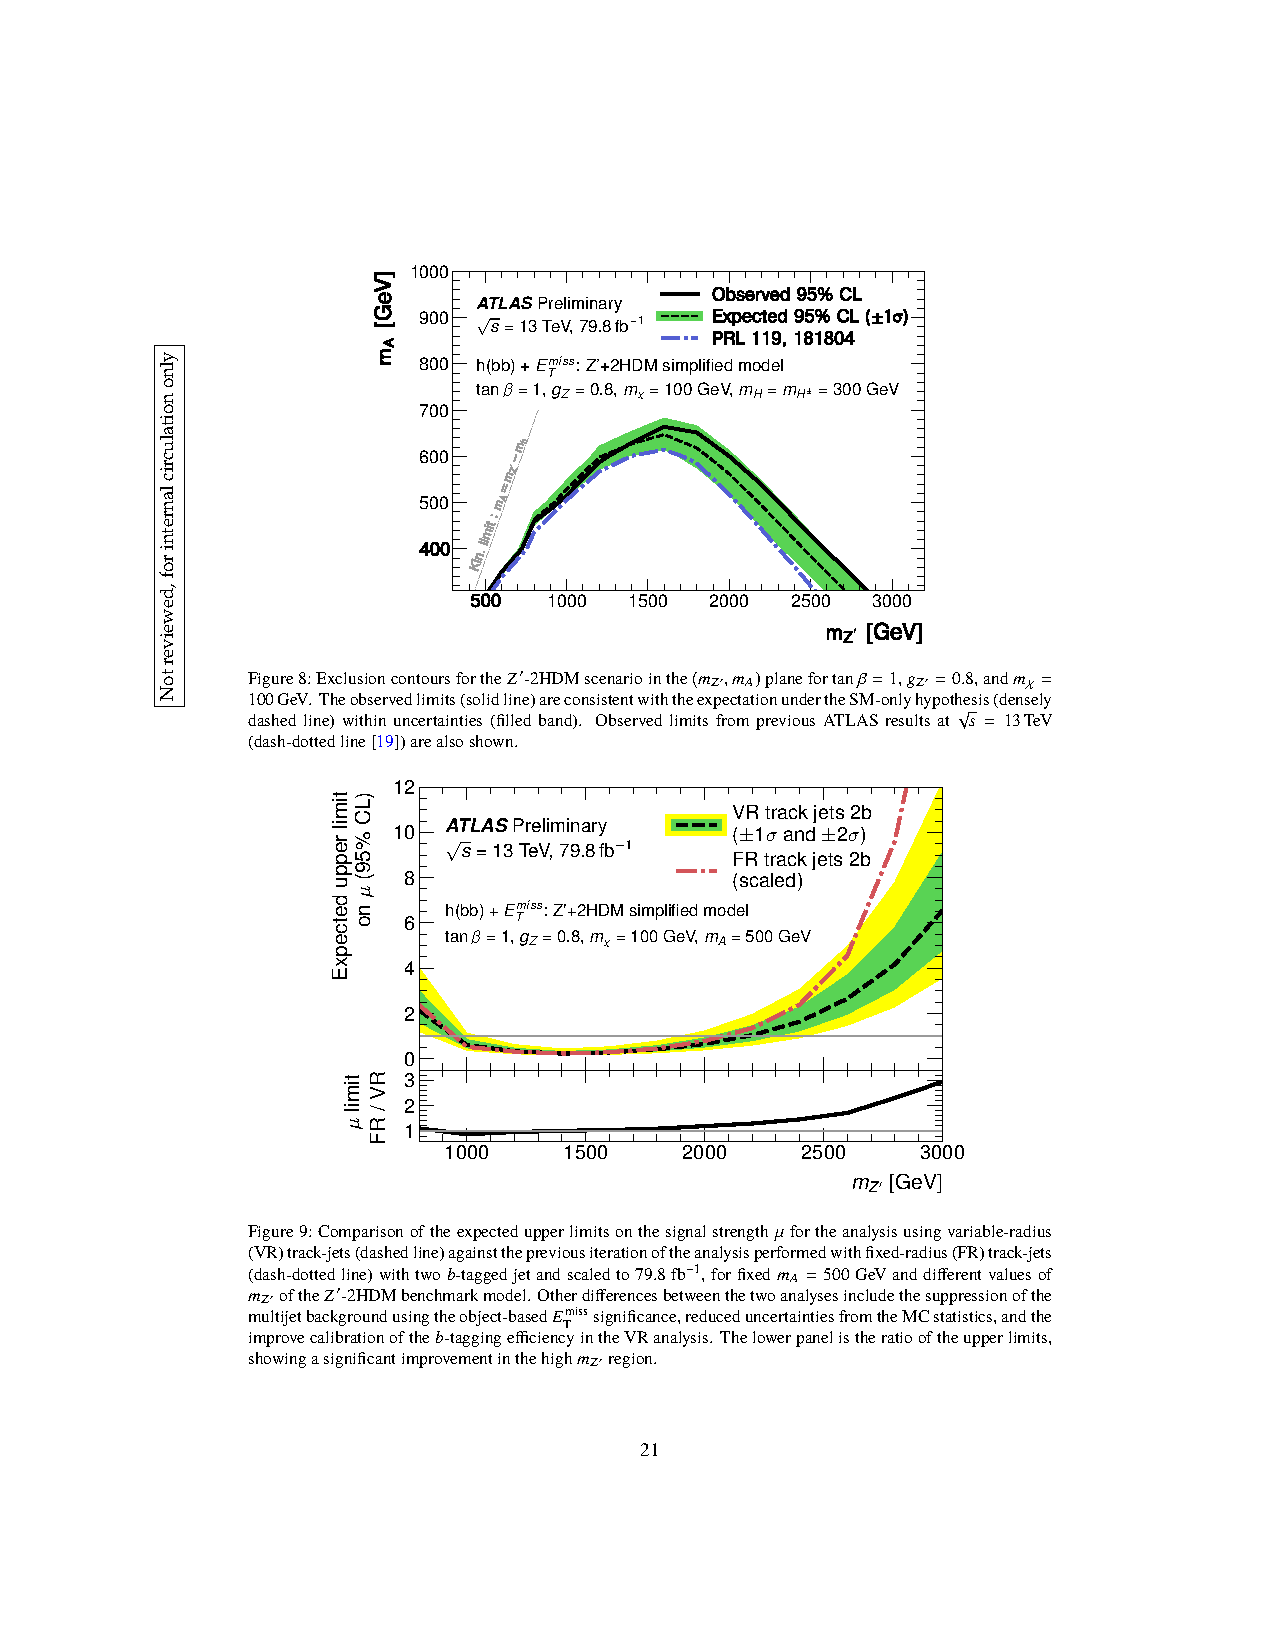
\includegraphics[width=12cm, height=9cm, trim={2.5cm 7.5cm 17.6cm 8cm}, clip]{chapters/c9/figures/ZPrime2HDMLimit.pdf}
    \caption{Fractional uncertainty on $\mu$ due to data statistics for each Z'-2HDM signal point.}
    \label{fig:zprime-2hdm-limit}
\end{figure}



\part{Conclusions}
\label{sec:conclusions}
\chapter{Conclusions}

\label{ch:con}

\par A search for dark matter coupled to Higgs boson has been presented in this thesis. 
The data sample, collected in 2015, 2016, 2017 and 2018 with ATLAS detector at the CERN large hadron collider (LHC), corresponds to an integrated luminosity of 139~\ifb. 

\par The standard model backgrounds are estimated using Monte-Carlo simulation and controlled by control regions. 
No excess of events above the expected standard model background is observed. 
The analysis result is interpreted in the context of simplified $Z\prime$+2HDM model as 95\% confidence level upper limits on cross section. 
Model parameters are constrained with newly collected data, which is a good guidance on the further theoretical development.


%%%
%%% Appendices
%%%
\part{Appendices}
\appendix
\chapter{CombinedXbbScore Tagger implementation}

\section{Performance}

\par The Boosted Xbb Tagger is based on a neural network (roughly 10 layers) which uses b-tagging and jet substructure information. 
The classification has three outputs which represent how likely the jet is Higgs, Top and QCD jet.  

\par With different fraction of the the three classes, CombinedXbbScore Tagger is defined as
\begin{equation}
D=ln(\frac{p_H}{(1-f)\times p_{QCD}+f\times p_{top}}),
\end{equation}
where f is the mixing fraction of top jet in the background, and XbbScore Top/Higgs/QCD are the three output of the Xbb Tagger.

\par The performance can be expressed in terms of its receiver operator characteristic (ROC) plot, which shows the change of background rejection as a function of the Higgs boson tagging efficiency. 
Fig.\ref{fig:roctop} compares CombinedXbbScore aggers with different mixing fraction.

\begin{figure}[h]
    \centering
    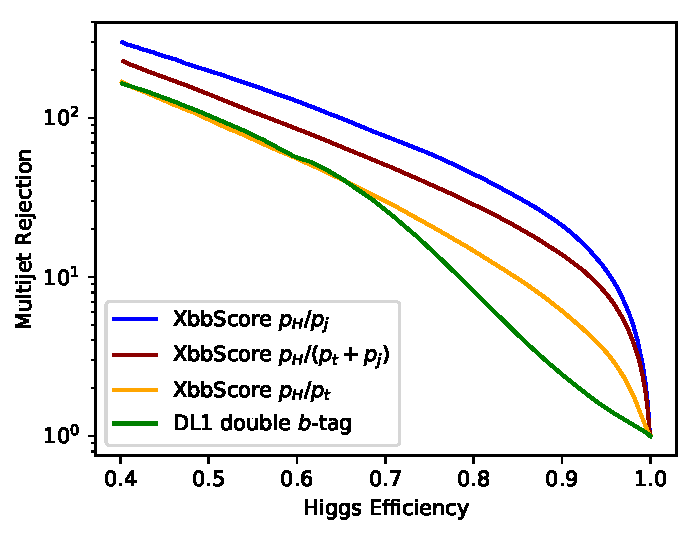
\includegraphics[width=0.4\textwidth]{appendices/figures/roc_multijet.pdf}
    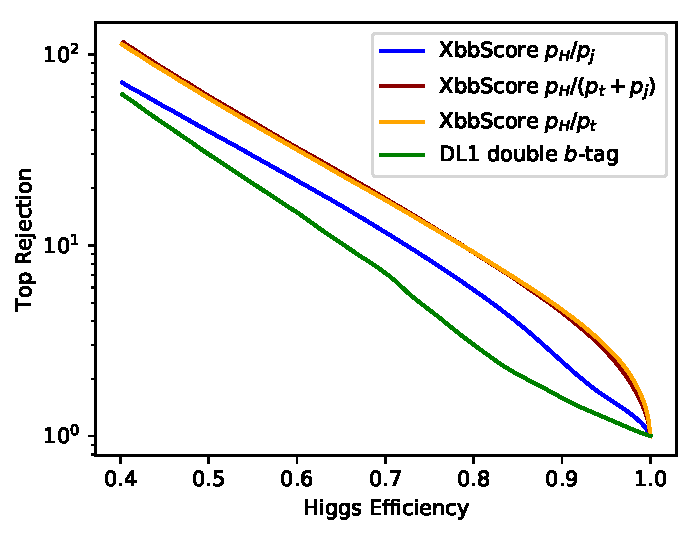
\includegraphics[width=0.4\textwidth]{appendices/figures/roc_top.pdf}
    \caption{ ROC plot: Comparison between different working points of CombinedXbbScore}
    \label{fig:roctop}
\end{figure}

\par The preliminary working points of the CombinedXbbScore are listed in Table.\ref{tab:combxbb}.

\begin{table}
    \footnotesize{
        \begin{center}
            \begin{tabular}{ c |c |c |c}
                \hline
                \hline
                Higgs efficiency [\%] & mixing fraction (f) & cut value \\
                50 & 0 & 5.1 \\
                60 & 0 & 4.8 \\
                70 & 0 & 3.9 \\
                50 & 0.2 & 4.5 \\
                60 & 0.2 & 3.9 \\
                70 & 0.2 & 3.0 \\
                50 & 1 & 3.6 \\
                60 & 1 & 3.0 \\
                70 & 1 & 2.1 \\
                \hline
                \hline
            \end{tabular}
        \end{center}
        }
    \caption{Preliminary working points of CombinedXbbScore}
    \label{tab:combxbb}
\end{table}

\section{Signal selection in Merged region using CombinedXbbScore}

\par For the merged region, instead of requiring two b-tagged VR track jets with 77\% working point as described in Section.\ref{sec:ana-sig:physobj}, cutting on the CombinedXbbScore of a large-R jet can choose the Xbb jets directly.
The background large-R jets (R = 1.0) is suppressed by applying a cut on CombinedXbbScore. 
To have a fair comparison within these two methods, 77\% working point is chosen for the VR track jets b-tagging and 60\% working points are chosen for the CombinedXbbScore tagger with different mixing fractions for all plots showed in this chapter.                    

\par The large-R jet mass distribution of the Z’+2HDM signal with $m_Z’ = 2800~GeV$ and $m_A = 300~GeV$ is scaled by a factor of 1000 and compared to backgrounds in both Fig.\ref{fig:mj_before} and Fig.\ref{fig:mj_after}.   

\par The left plot in Fig.\ref{fig:mj_before} shows the large-R jet mass distribution in the merged region while the right plot shows the large-R jet mass distribution after requiring two b-tagged VR track jets. 
Fig.\ref{fig:mj_before} shows the large-R jet mass distribution after applying cutting on CombinedXbbScore with mixing fraction $f=1$ (left) and $f=0$ (right).     

\begin{figure}[h]
    \centering
    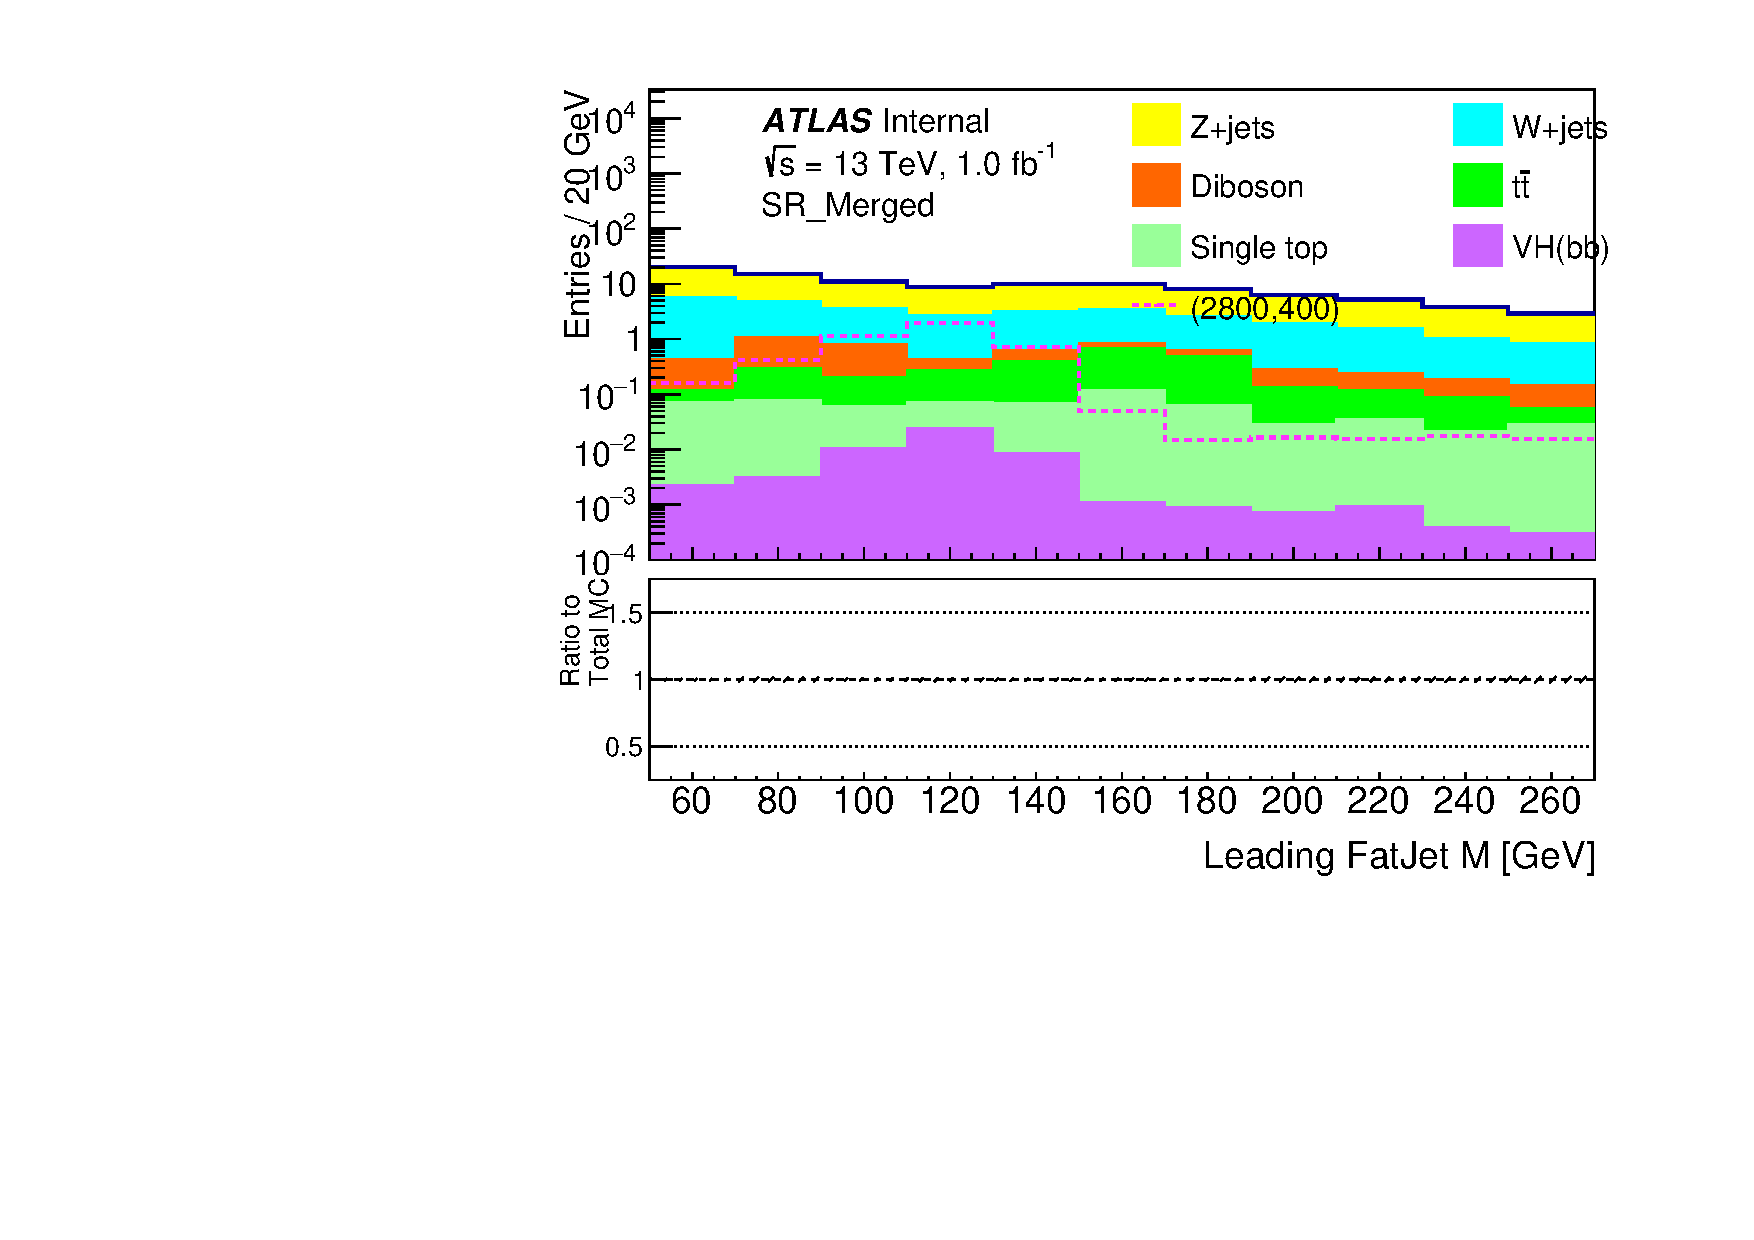
\includegraphics[width=0.4\textwidth]{appendices/figures/MC_MonoH_Nominal_SR_Merged_fatjets_m1_20GeV_LogY.pdf}
    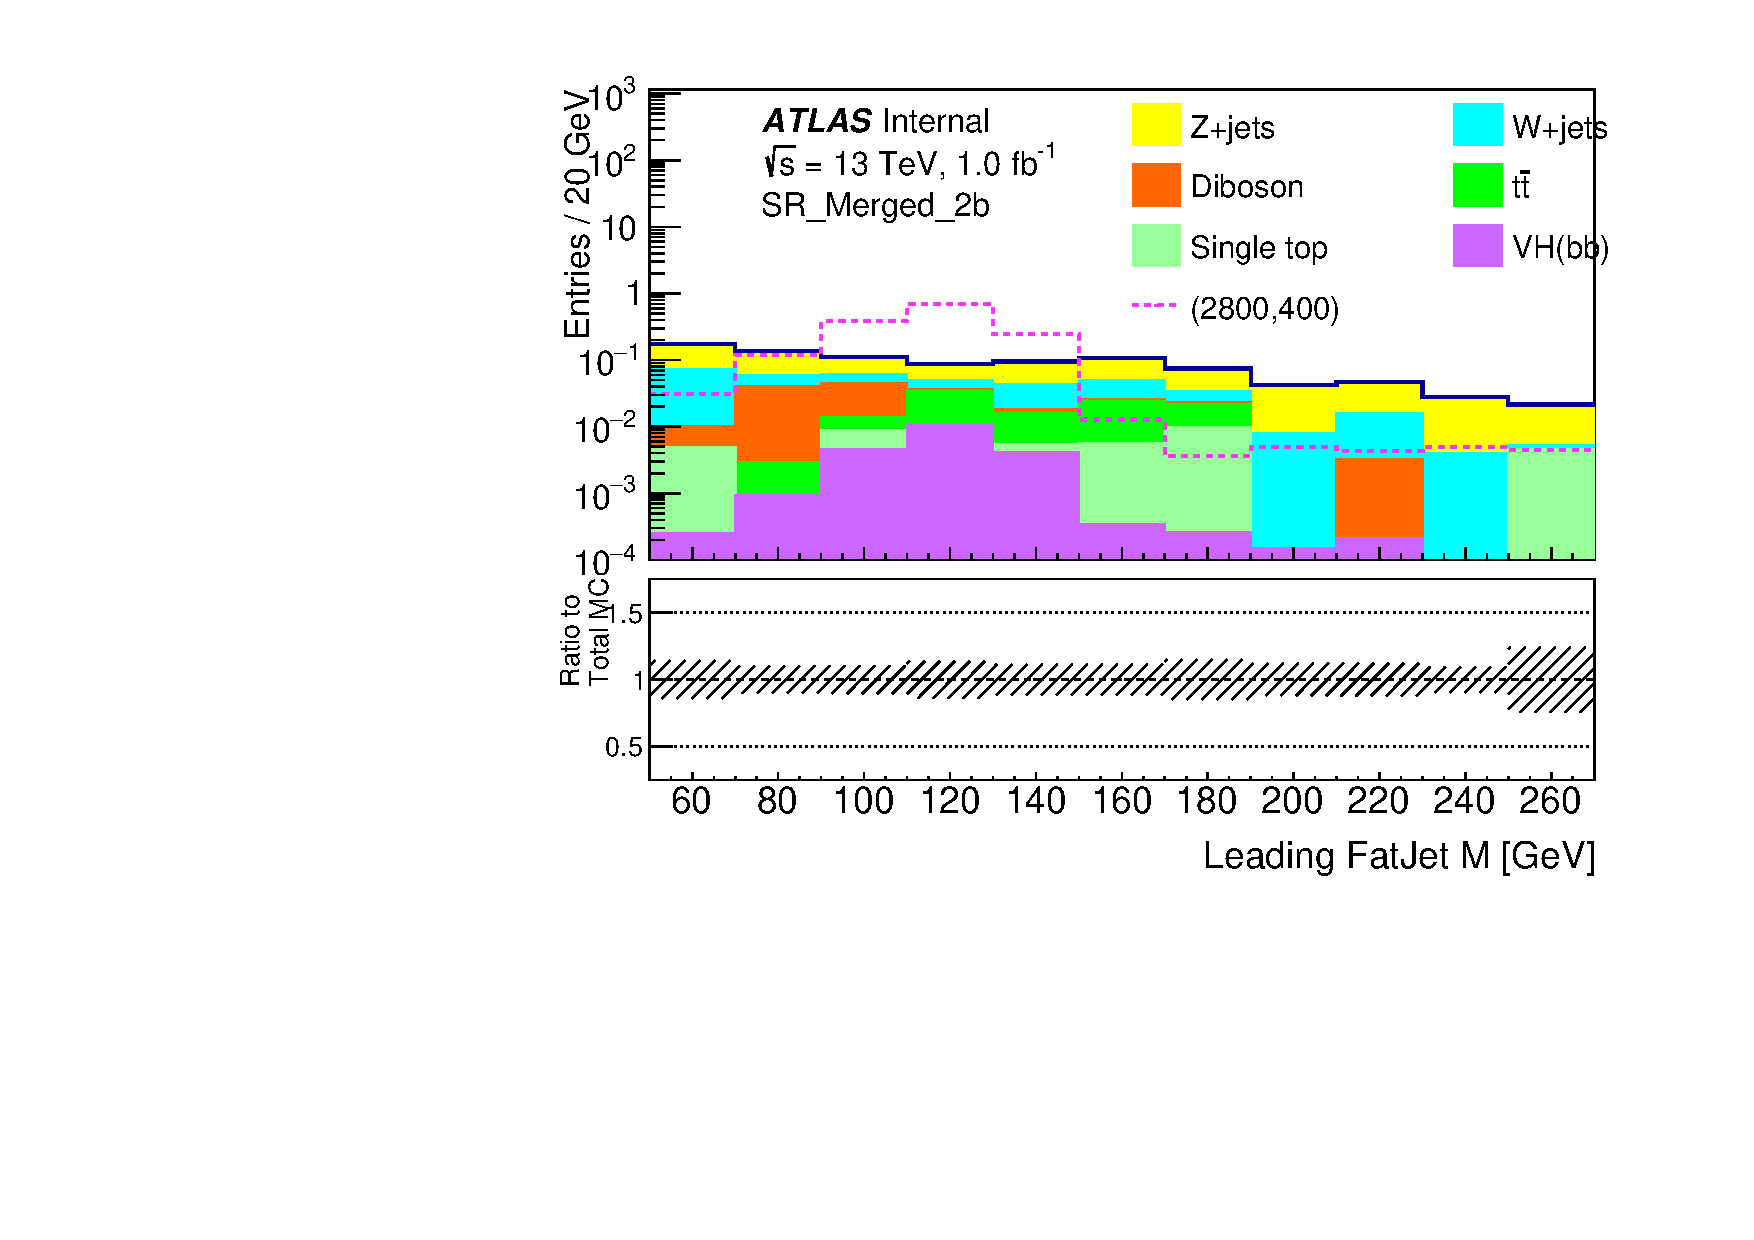
\includegraphics[width=0.4\textwidth]{appendices/figures/MC_MonoH_Nominal_SR_Merged_2b_fatjets_m1_20GeV_LogY_vr.pdf}
    \caption{Leading Fatjet mass in Merged region (left) and 2b Merged region defined by 2-b tagged VR (right)}
    \label{fig:mj_before}
\end{figure}

\begin{figure}[h]
    \centering
    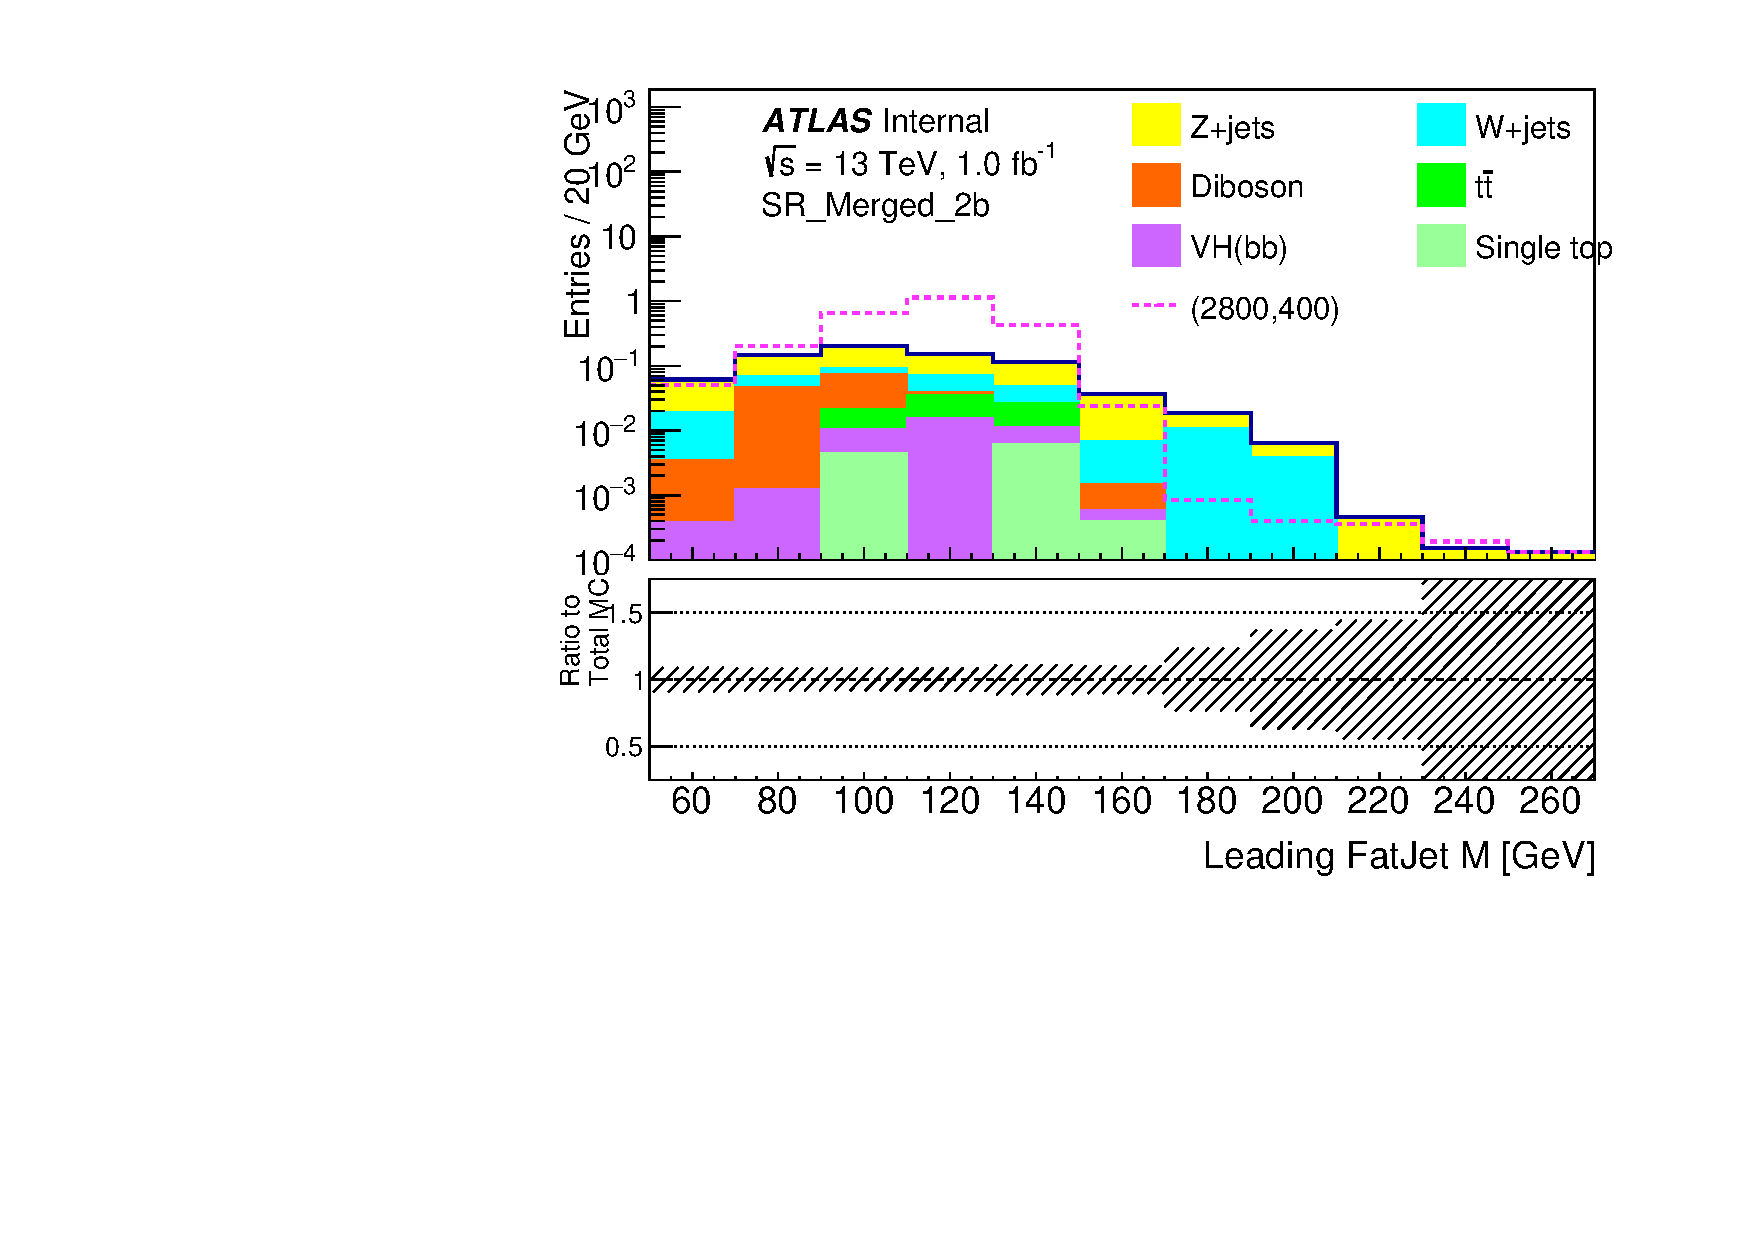
\includegraphics[width=0.4\textwidth]{appendices/figures/MC_MonoH_Nominal_SR_Merged_2b_fatjets_m1_20GeV_LogY_xbb.pdf}
    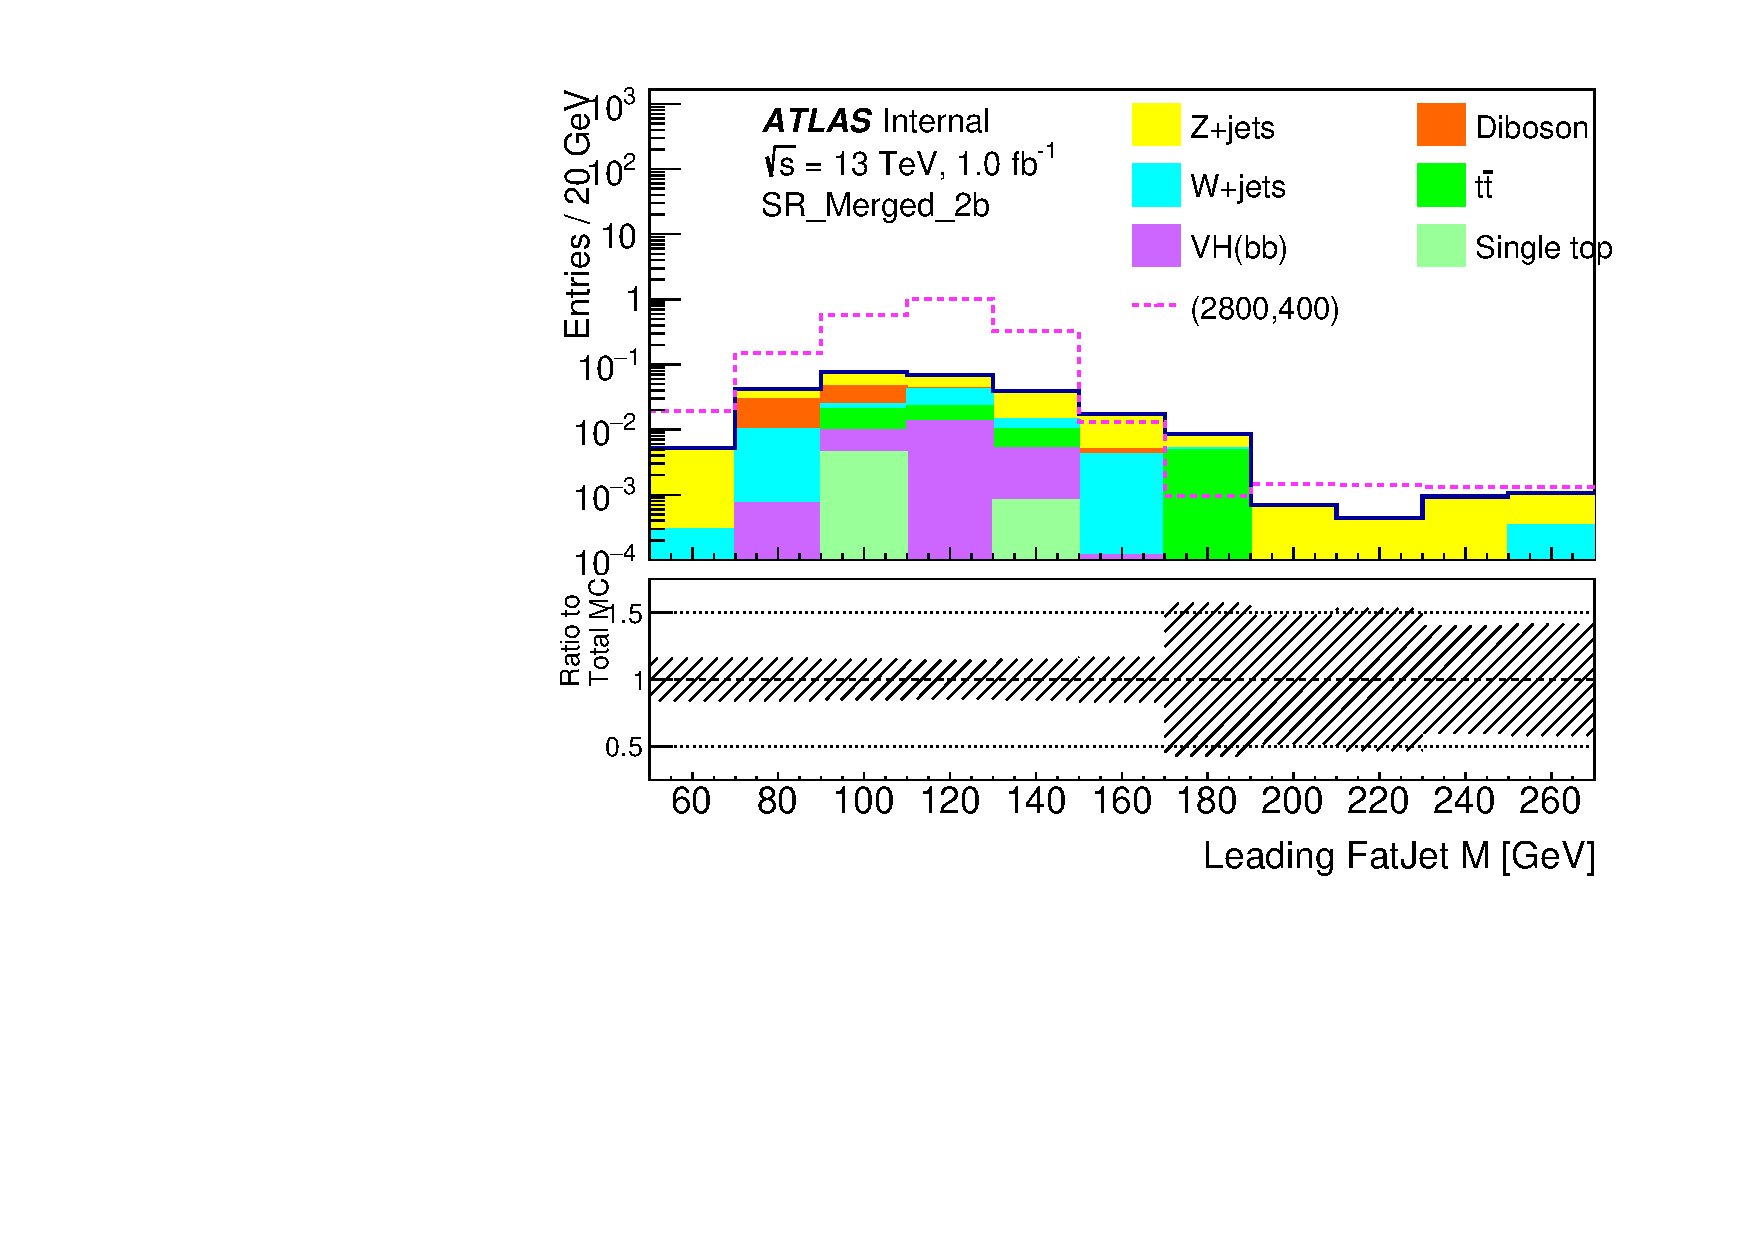
\includegraphics[width=0.4\textwidth]{appendices/figures/MC_MonoH_Nominal_SR_Merged_2b_fatjets_m1_20GeV_LogY_xbb_f0.pdf}
    \caption{Leading Fatjet mass in 2b Merged region defined by CombinedXbbScore}
    \label{fig:mj_after}
\end{figure}

\par While the CombinedXbbScore tagger did a much better job at suppressing backgrounds, it also shaped the background distributions. 

\subsection{Backgrounds breakdown of signal region and control regions}

\par To study the modeling and systematics, truth labeling is implemented in ntuples based on the truth particles ghost-associated to the large-R jets.
And the composition of the background on the 1L/2L control regions is examined.

\par Fig.\ref{fig:fl_mj} shows the large-R jet mass distribution in the 2b-tagged signal and control regions defined by the CombinedXbbScore.

\begin{figure}[h]
    \centering
    \includegraphics[width=0.4\textwidth]{appendices/figures/Region_BMin500_incFat1_Fat1_incJet1_Y2015_DSR_T2_L0_distmBB_J0_Prefit.pdf}
    \includegraphics[width=0.4\textwidth]{appendices/figures/Region_BMin500_incFat1_Fat1_incJet1_Y2015_DCR1_T2_L1_distCharge_J0_Prefit.pdf}
    \includegraphics[width=0.4\textwidth]{appendices/figures/Region_BMin500_incFat1_Fat1_incJet1_Y2015_DCR2_T2_L2_distmBB_J0_Prefit.pdf}
    \caption{Large-R jet mass distribution in the 2-btagged signal and control regions.}
    \label{fig:fl_mj}
\end{figure}

\par Ideally, large-R jets selected by cutting on CombinedXbbScore are likely to have two b-hadrons ghost-associated to them and have a truth labeling of bb.

\par To have a clear look at the fraction of large-R jets labeling, the Xbb tag fraction which refers to the fraction of large-R jets with labeling bb are examined for 1 lepton region with W+jets samples in Fig.\ref{fig:xbbw} and for 2 regions with Z+jets samples in Fig.\ref{fig:xbbz}.

\begin{figure}[h]
    \centering
    \includegraphics[width=0.45\textwidth]{appendices/figures/eff_W}
    \includegraphics[width=0.45\textwidth]{appendices/figures/eff_Wnon}
    \caption{Fraction of large-R jets with bb labeling (left) and without bb labeling (right) in with W+jets samples.}
    \label{fig:xbbw}
\end{figure}

\begin{figure}[h]
    \centering
    \includegraphics[width=0.45\textwidth]{appendices/figures/eff_Z}
    \includegraphics[width=0.45\textwidth]{appendices/figures/eff_Znon}
    \caption{Fraction of large-R jets with bb labeling (left) and without bb labeling (right) in with Z+jets samples.}
    \label{fig:xbbz}
\end{figure}

\par Xbb tag fraction of signal region vs 1b control regions in Fig.\ref{fig:xbbw} matches within uncertainty, as well as signal region vs 2b control regions in Fig.\ref{fig:xbbz}.
And the Xbb tag fraction peaks in around Higgs mass.

\par The flavor breakdown of backgrounds with truth labeling in signal and control regions is showed in Fig.\ref{fig:fl_pie}.

\begin{figure}[h]
    \includegraphics[ width=0.3\textwidth]{appendices/figures/pie0.pdf}
    \includegraphics[ width=0.3\textwidth]{appendices/figures/pie1.pdf}
    \includegraphics[ width=0.3\textwidth]{appendices/figures/pie2.pdf}
    \caption{Flavor breakdown of backgrounds with truth labeling in signal and control regions.}
    \label{fig:fl_pie}
\end{figure}

\par To further quantify the flavor breakdown in signal and control regions are showed in Table.\ref{tab:fl0}, Table.\ref{tab:fl1} and Table.\ref{tab:fl2}.

\begin{table}
    \centering
    \tiny
    \begin{tabular}{l|c|}
    \cline{2-2} & \multicolumn{1}{c|}{Zero lepton 2 tag merged,~$E_{T}^{miss}$$ >$ 500 GeV} \\
    \hline
    signal mzp1400\_mA600 & 0.0458$\pm$0.0005 \\
    \hline
    WZ    & 0.6106$\pm$0.2170 \\
    ZZ    & 3.9200$\pm$0.3486 \\
    Wl    & 0.4992$\pm$0.2104 \\
    Wcl   & 0.2709$\pm$0.0918 \\
    Wbb   & 1.3348$\pm$0.2478 \\
    Wbl   & 0.7481$\pm$0.1999 \\
    Wbc   & 0.0100$\pm$0.0070 \\
    Zl    & 0.3124$\pm$0.0293 \\
    VHbb  & 1.5404$\pm$0.0162 \\
    WW    & 0.1818$\pm$0.1285 \\
    Zcc   & 0.3775$\pm$0.0293 \\
    Zbl   & 1.5497$\pm$0.0580 \\
    Zbb   & 3.8587$\pm$0.0879 \\
    Zcl   & 0.4465$\pm$0.0431 \\
    Zbc   & 0.2807$\pm$0.0233 \\
    ttbar & 6.0874$\pm$0.2225 \\
    stopWt& 1.5491$\pm$0.4528 \\
    stops & 0.0200$\pm$0.0141 \\
    \hline
    Total Bkgd & 23.5977$\pm$3.3084 \\
    \hline
    \end{tabular}
    \caption{Flavor breakdown of backgrounds with truth labeling in signal region.}
    \label{tab:fl0}
\end{table}

\begin{table}
    \centering
    \tiny
    \begin{tabular}{l|c|}
        \cline{2-2} & \multicolumn{1}{c|}{One lepton 2 tag merged,~$E_{T}^{miss}$$ >$ 500 GeV} \\
        \hline
        WZ    & 1.7570$\pm$0.2641 \\
        ZZ    & 0.0775$\pm$0.0264 \\
        Wl    & 0.2212$\pm$0.0978 \\
        Wcl   & 0.5467$\pm$0.2127 \\
        Wbb   & 4.8836$\pm$0.5282 \\
        Wcc   & 0.5283$\pm$0.1443 \\
        Wbl   & 1.5783$\pm$0.2929 \\
        Wbc   & 0.8691$\pm$0.2415 \\
        Zl    & 0.0060$\pm$0.0043 \\
        VHbb  & 1.5967$\pm$0.0162 \\
        Zbl   & 0.0093$\pm$0.0093 \\
        Zbb   & 0.0333$\pm$0.0276 \\
        ttbar & 28.449$\pm$0.8372 \\
        stopWt& 9.6438$\pm$1.1237 \\
        stops & 0.0704$\pm$0.0321 \\
        \hline
        Total Bkgd & 50.2699$\pm$3.1672 \\
        \hline
    \end{tabular}
    \caption{Flavor breakdown of backgrounds with truth labeling in 1 lepton control region.}
    \label{tab:fl1}
\end{table}    

\begin{table}
    \centering
    \tiny
    \begin{tabular}{l|c|}
        \cline{2-2} & \multicolumn{1}{c|}{Two lepton 2 tag merged, $E_{T}^{miss}$ $>$ 500 GeV} \\
        \hline
        WZ    & 0.1108$\pm$0.0427 \\
        ZZ    & 0.7880$\pm$0.1048 \\
        Zl    & 0.2722$\pm$0.1364 \\
        VHbb  & 0.4736$\pm$0.0053 \\
        Zcc   & 0.0991$\pm$0.0360 \\
        Zbl   & 0.6740$\pm$0.0969 \\
        Zbb   & 1.6105$\pm$0.1363 \\
        Zcl   & 0.1514$\pm$0.0428 \\
        Zbc   & 0.1524$\pm$0.0404 \\
        \hline
        Total Bkgd & 4.3320$\pm$ 5.8464 \\
        \hline
    \end{tabular}
    \caption{Flavor breakdown of backgrounds with truth labeling in 2 lepton control region.}
    \label{tab:fl2}
\end{table}

\par According to the tables above, the Wbb fraction in W+jets in the signal region is 46.62\% $\pm$ 10.76\% compared to 56.60\% $\pm$ 7.68\% in 1 lepton control region. 
And the Zbb fraction in Z+jets is 56.53\%$\pm$1.64\% compared to 54.42\%$\pm$6.21\% in 2 lepton control region.

\subsection{Preliminary significance study}

\par To quantify the improvement brought by the CombinedXbbScore, the signal significances of these two methods are compared.
Signal Significance in each bin is defined as
\begin{equation}
    S_i = \sqrt{2(s + b)ln(1 + \frac{s}{b}) − s},
\end{equation}
where s, b is the count of signal and background in the i-th bin.

\par And the Bin-by-bin signal significance is defined as
\begin{equation}
    S_{bin-by-bin} = \sqrt{\sum_i S_i^2}, 
\end{equation}

\par Fig.\ref{fig:ss_ratio} (left) shows the ratio of the signal significance of the 2b region defined by CombinedXbbScore vs 2b b-tagged VR track jets with the Higgs window [70, 140]~GeV,
while the right plot is without the Higgs window.
\begin{figure}[h]
    \centering
    \includegraphics[width=0.45\textwidth]{appendices/figures/2b-tags_XbbScoreoverVR_HiggsWindow.pdf}
    \includegraphics[width=0.45\textwidth]{appendices/figures/2b-tags_XbbScoreoverVR.pdf}
    \caption{Ratio of signal significance of 2b merged region defined by CombinedXbbScore compared to the original method with or without the Higgs window.}
    \label{fig:ss_ratio}
\end{figure}

\chapter{Analysis supplementary materials}

Sample text sample text sample text. Sample text sample text sample text.
Sample text sample text sample text. Sample text sample text sample text.
Sample text sample text sample text. Sample text sample text sample text.
Sample text sample text sample text. Sample text sample text sample text.
Sample text sample text sample text. Sample text sample text sample text.
Sample text sample text sample text. Sample text sample text sample text.

\section{$pp \rightarrow Hb\bar{b}$}
Sample text sample text sample text. Sample text sample text sample text.
Sample text sample text sample text. Sample text sample text sample text.
Sample text sample text sample text. Sample text sample text sample text.

\subsection{Sample subsection}
Sample text sample text sample text. Sample text sample text sample text.
Sample text sample text sample text. Sample text sample text sample text.
Sample text sample text sample text. Sample text sample text sample text.

\subsection{Sample subsubsection}
Sample text sample text sample text. Sample text sample text sample text.
Sample text sample text sample text. Sample text sample text sample text.
Sample text sample text sample text. Sample text sample text sample text.

\section{$pp \rightarrow q\bar{q}b\bar{b}$}
Sample text sample text sample text. Sample text sample text sample text.
Sample text sample text sample text. Sample text sample text sample text.
Sample text sample text sample text. Sample text sample text sample text.

\subsection{Sample subsection}
Sample text sample text sample text. Sample text sample text sample text.
Sample text sample text sample text. Sample text sample text sample text.
Sample text sample text sample text. Sample text sample text sample text.


%%%
%%% Bibliography
%%%
\part{Bibliography}
\addcontentsline{toc}{chapter}{Bibliography}
\bibliography{reference}
\bibliographystyle{named}

\end{document}
